\documentclass[pdf]{beamer}\usepackage[]{graphicx}\usepackage[]{color}
%% maxwidth is the original width if it is less than linewidth
%% otherwise use linewidth (to make sure the graphics do not exceed the margin)
\makeatletter
\def\maxwidth{ %
  \ifdim\Gin@nat@width>\linewidth
    \linewidth
  \else
    \Gin@nat@width
  \fi
}
\makeatother

\definecolor{fgcolor}{rgb}{0.345, 0.345, 0.345}
\newcommand{\hlnum}[1]{\textcolor[rgb]{0.686,0.059,0.569}{#1}}%
\newcommand{\hlstr}[1]{\textcolor[rgb]{0.192,0.494,0.8}{#1}}%
\newcommand{\hlcom}[1]{\textcolor[rgb]{0.678,0.584,0.686}{\textit{#1}}}%
\newcommand{\hlopt}[1]{\textcolor[rgb]{0,0,0}{#1}}%
\newcommand{\hlstd}[1]{\textcolor[rgb]{0.345,0.345,0.345}{#1}}%
\newcommand{\hlkwa}[1]{\textcolor[rgb]{0.161,0.373,0.58}{\textbf{#1}}}%
\newcommand{\hlkwb}[1]{\textcolor[rgb]{0.69,0.353,0.396}{#1}}%
\newcommand{\hlkwc}[1]{\textcolor[rgb]{0.333,0.667,0.333}{#1}}%
\newcommand{\hlkwd}[1]{\textcolor[rgb]{0.737,0.353,0.396}{\textbf{#1}}}%
\let\hlipl\hlkwb

\usepackage{framed}
\makeatletter
\newenvironment{kframe}{%
 \def\at@end@of@kframe{}%
 \ifinner\ifhmode%
  \def\at@end@of@kframe{\end{minipage}}%
  \begin{minipage}{\columnwidth}%
 \fi\fi%
 \def\FrameCommand##1{\hskip\@totalleftmargin \hskip-\fboxsep
 \colorbox{shadecolor}{##1}\hskip-\fboxsep
     % There is no \\@totalrightmargin, so:
     \hskip-\linewidth \hskip-\@totalleftmargin \hskip\columnwidth}%
 \MakeFramed {\advance\hsize-\width
   \@totalleftmargin\z@ \linewidth\hsize
   \@setminipage}}%
 {\par\unskip\endMakeFramed%
 \at@end@of@kframe}
\makeatother

\definecolor{shadecolor}{rgb}{.97, .97, .97}
\definecolor{messagecolor}{rgb}{0, 0, 0}
\definecolor{warningcolor}{rgb}{1, 0, 1}
\definecolor{errorcolor}{rgb}{1, 0, 0}
\newenvironment{knitrout}{}{} % an empty environment to be redefined in TeX

\usepackage{alltt}
\mode<presentation>
\usetheme[compress]{Singapore} %Berkeley, Palo Alto, Singapore, Warsaw
%\usetheme[compress]{Berlin} 
%\usetheme[compress]{Madrid} 
%\usecolortheme{seagull}  %Beaver, dolphin, dove, lily, orchid, seagull, seahorse

%\usefonttheme{serif}
% font themes: default, professionalfonts, serif, structurebold, structureitalicserif, structuresmallcapsserif

\usepackage{graphicx}
\usepackage{pgf}
\usepackage{array}
\usepackage{tabularx}
\usepackage{booktabs}          %% Used in risk tables
\usepackage{multirow}          %% Used in decision tables
\usepackage{multicol}          %% Used in the toc
\usepackage[T1]{fontenc}  %to use < or > in tables

%\graphicspath{C:/Users/Chantel.Wetzel/Documents/GitHub/POP_2017}
\newcolumntype{Y}{>{\centering\arraybackslash}X}
\newcommand{\specialcell}[2][c]{\begin{tabular}[#1]{@{}c@{}}#2\end{tabular}}
\newcommand{\subscr}[1]{$_{\text{#1}}$}
\newcommand{\Fforty}{F_{\text{SPR}=40\%}}       % Needs to be done as $\Fforty$
\newcommand{\Bforty}{B_{\text{SPR}=40\%}}

\setbeamersize{text margin left=0.1in}
\setbeamersize{text margin right=0.1in}

\definecolor{pageCol}{rgb}{0.5,0.5,1.0}

\usepackage{tikz}

\usebackgroundtemplate{
  \tikz[overlay,remember picture] 
  \node[opacity=0.3, at=(current page.south east),anchor=south east,inner sep=0pt] {
    
\includegraphics[height=0.5in]{noaalogo.jpg}};
}

\setbeamertemplate{footline}
{
  \begin{beamercolorbox}[wd=.05\paperwidth,ht=0ex,dp=0ex,left]{framenumber in head/foot}%
    \insertframenumber/\inserttotalframenumber
    
  \end{beamercolorbox}%
}
\setbeamercolor{footline}{fg=pageCol}

\newcounter{saveenumi}

%<<load_everything, echo = FALSE, message=FALSE, results='hide', warning=FALSE>>=
%     source("C:/Users/Chantel.Wetzel/Documents/GitHub/POP_2017/Presentation/0_Run_Model_Presentation.R")
%      #create.plots = TRUE
%      #Run.Model.Present(create.plots)
%     source("C:/Users/Chantel.Wetzel/Documents/GitHub/POP_2017/Presentation/tables/catch.R")
%@

\newcommand{\mytableofcontents}{
  \begin{frame}[t]
  \frametitle{Outline}
  \begin{multicols}{2}
  \tableofcontents[
    currentsection, sectionstyle=show/show, subsectionstyle=show/show/hide,
  ]
  \end{multicols}
  \end{frame}
}
\AtBeginSection[]{\mytableofcontents}

%------------------------------------------------------------------------------------
% Title Page
%------------------------------------------------------------------------------------
\title{Pacific ocean perch 2017 Assessment}
\subtitle{Biology and Data}
\author{Chantel Wetzel$^{1}$\\
        Lee Cronin-Fine$^{2}$}
\institute[NWFSC]{
Northwest Fisheries Science Center$^1$ \\
University of Washington$^2$ \\
\medskip
}
\date{{\footnotesize STAR Panel \\ June 26-30, 2017}}
\IfFileExists{upquote.sty}{\usepackage{upquote}}{}
\begin{document}

\begin{frame}
  \titlepage
\end{frame}


%------------------------------------------------------------------------------------
\section{Model Summary}
%------------------------------------------------------------------------------------
\subsection{Landings}
\begin{frame}{Landings}
  \begin{center}
    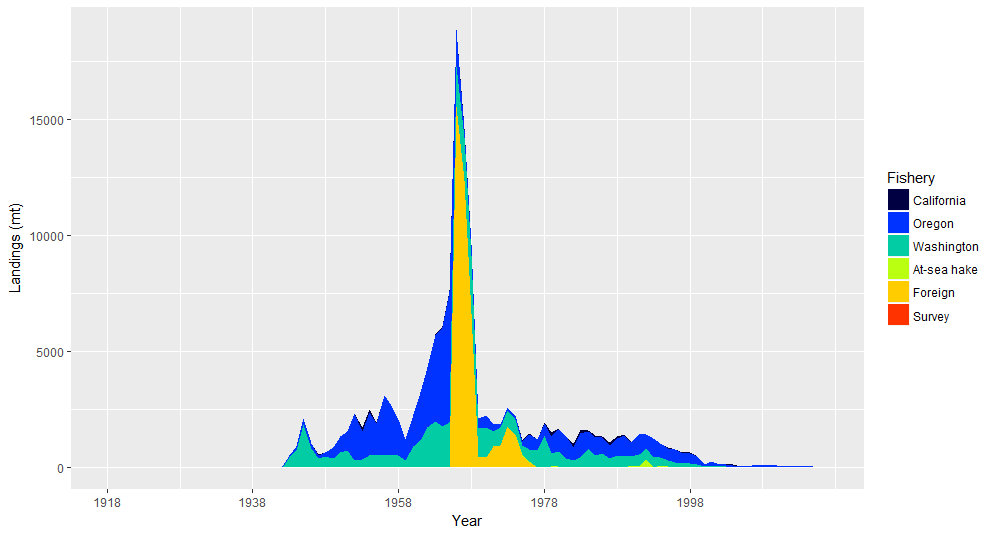
\includegraphics[scale = 0.40]{figures/catches.png}
  \end{center}
\end{frame}

\begin{frame}[t]
  %\input{tables/recent_catches.rnw}
  \begin{table}[ht]
  \centering
  %\begin{tabular}{l>{\centering}p{0.25in}>{\centering}p{0.25in}>{\centering}p{0.1in}>{\centering}p{0.1in}>{\centering}p{0.1in}>{\centering}p{0.1in}}
  \begin{tabular}{p{0.4in}p{0.4in}p{0.4in}p{0.4in}p{0.4in}p{0.4in}p{0.6in}}
  Year & CA & OR & WA & At-sea & Survey & Total Landings \\ 
  \hline
  2007 & 0.15 & 83.65 & 45.12 & 4.05 & 0.58 & 133.55 \\ 
  2008 & 0.39 & 58.64 & 16.61 & 15.93 & 0.80 & 92.36 \\ 
  2009 & 0.92 & 58.74 & 33.22 & 1.56 & 2.72 & 97.17 \\ 
  2010 & 0.14 & 58.00 & 22.29 & 16.87 & 1.68 & 98.98 \\ 
  2011 & 0.12 & 30.26 & 19.66 & 9.17 & 1.94 & 61.14 \\ 
  2012 & 0.18 & 30.41 & 21.79 & 4.52 & 1.62 & 58.51 \\ 
  2013 & 0.08 & 34.86 & 14.83 & 5.41 & 1.71 & 56.89 \\ 
  2014 & 0.18 & 33.91 & 15.82 & 3.92 & 0.57 & 54.40 \\ 
  2015 & 0.12 & 38.05 & 11.41 & 8.71 & 1.59 & 59.88 \\ 
  2016 & 0.23 & 40.81 & 13.12 & 10.30 & 3.10 & 67.56 \\ 
  \hline
  \end{tabular}
  \end{table}
\end{frame}


\subsection{Estimated Stock Size and Status}
\begin{frame}{Spawning Output}
  \begin{center}
    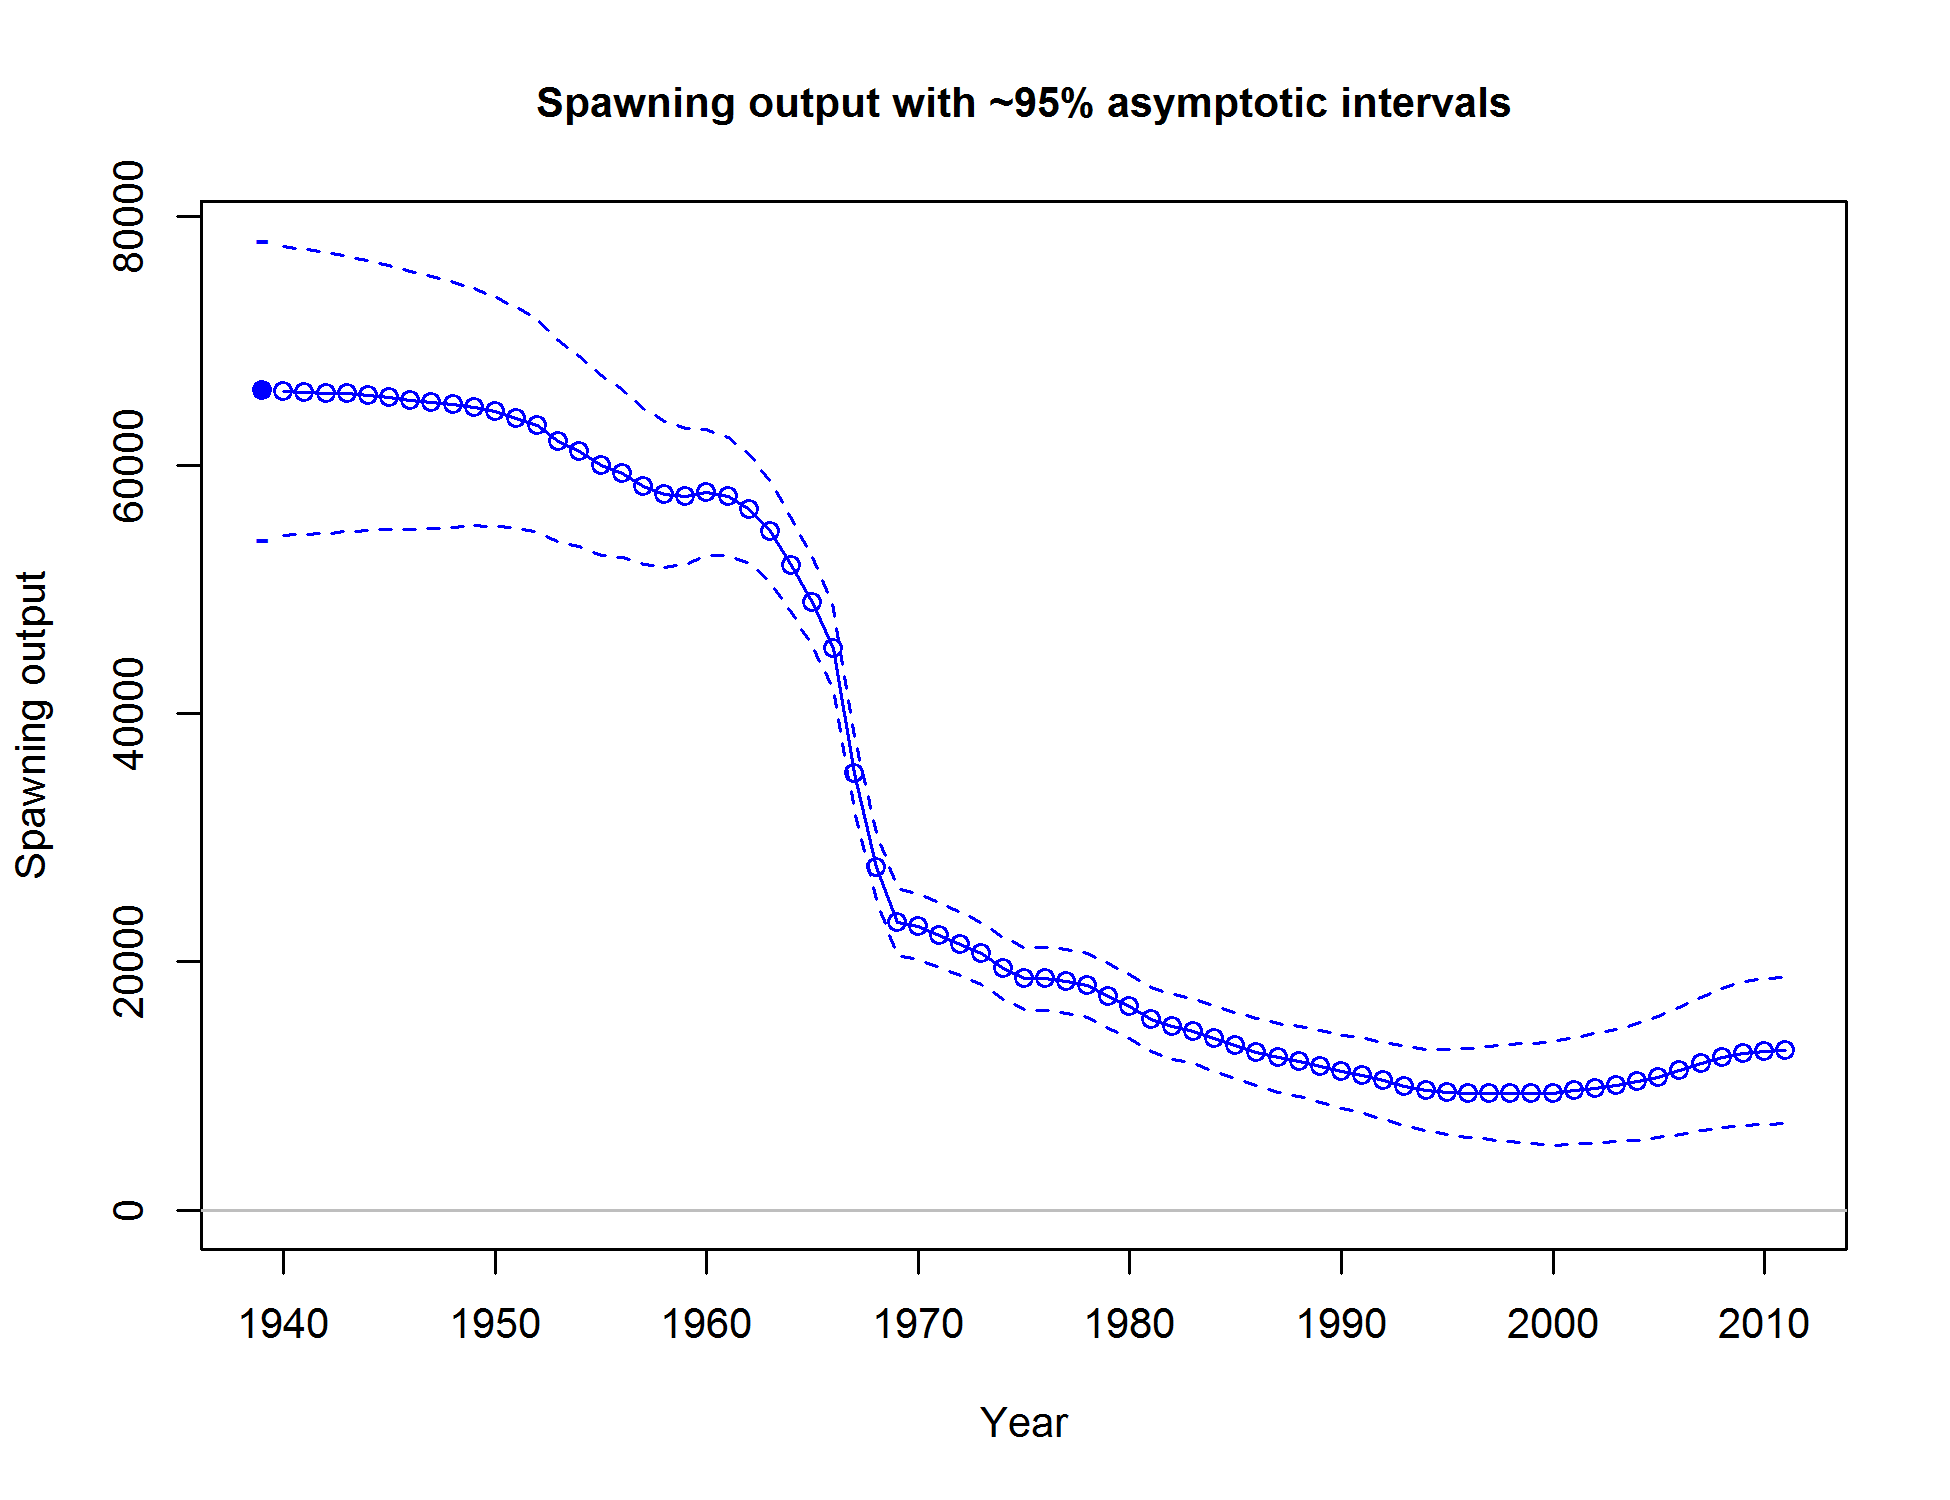
\includegraphics[scale = 0.50, trim={0cm 0cm 0cm 1.7cm}, clip]{r4ss/ts7_Spawning_output_with_95_asymptotic_intervals_intervals.png}
  \end{center}
\end{frame}


\begin{frame}{Relative Biomass}
  \begin{center}
    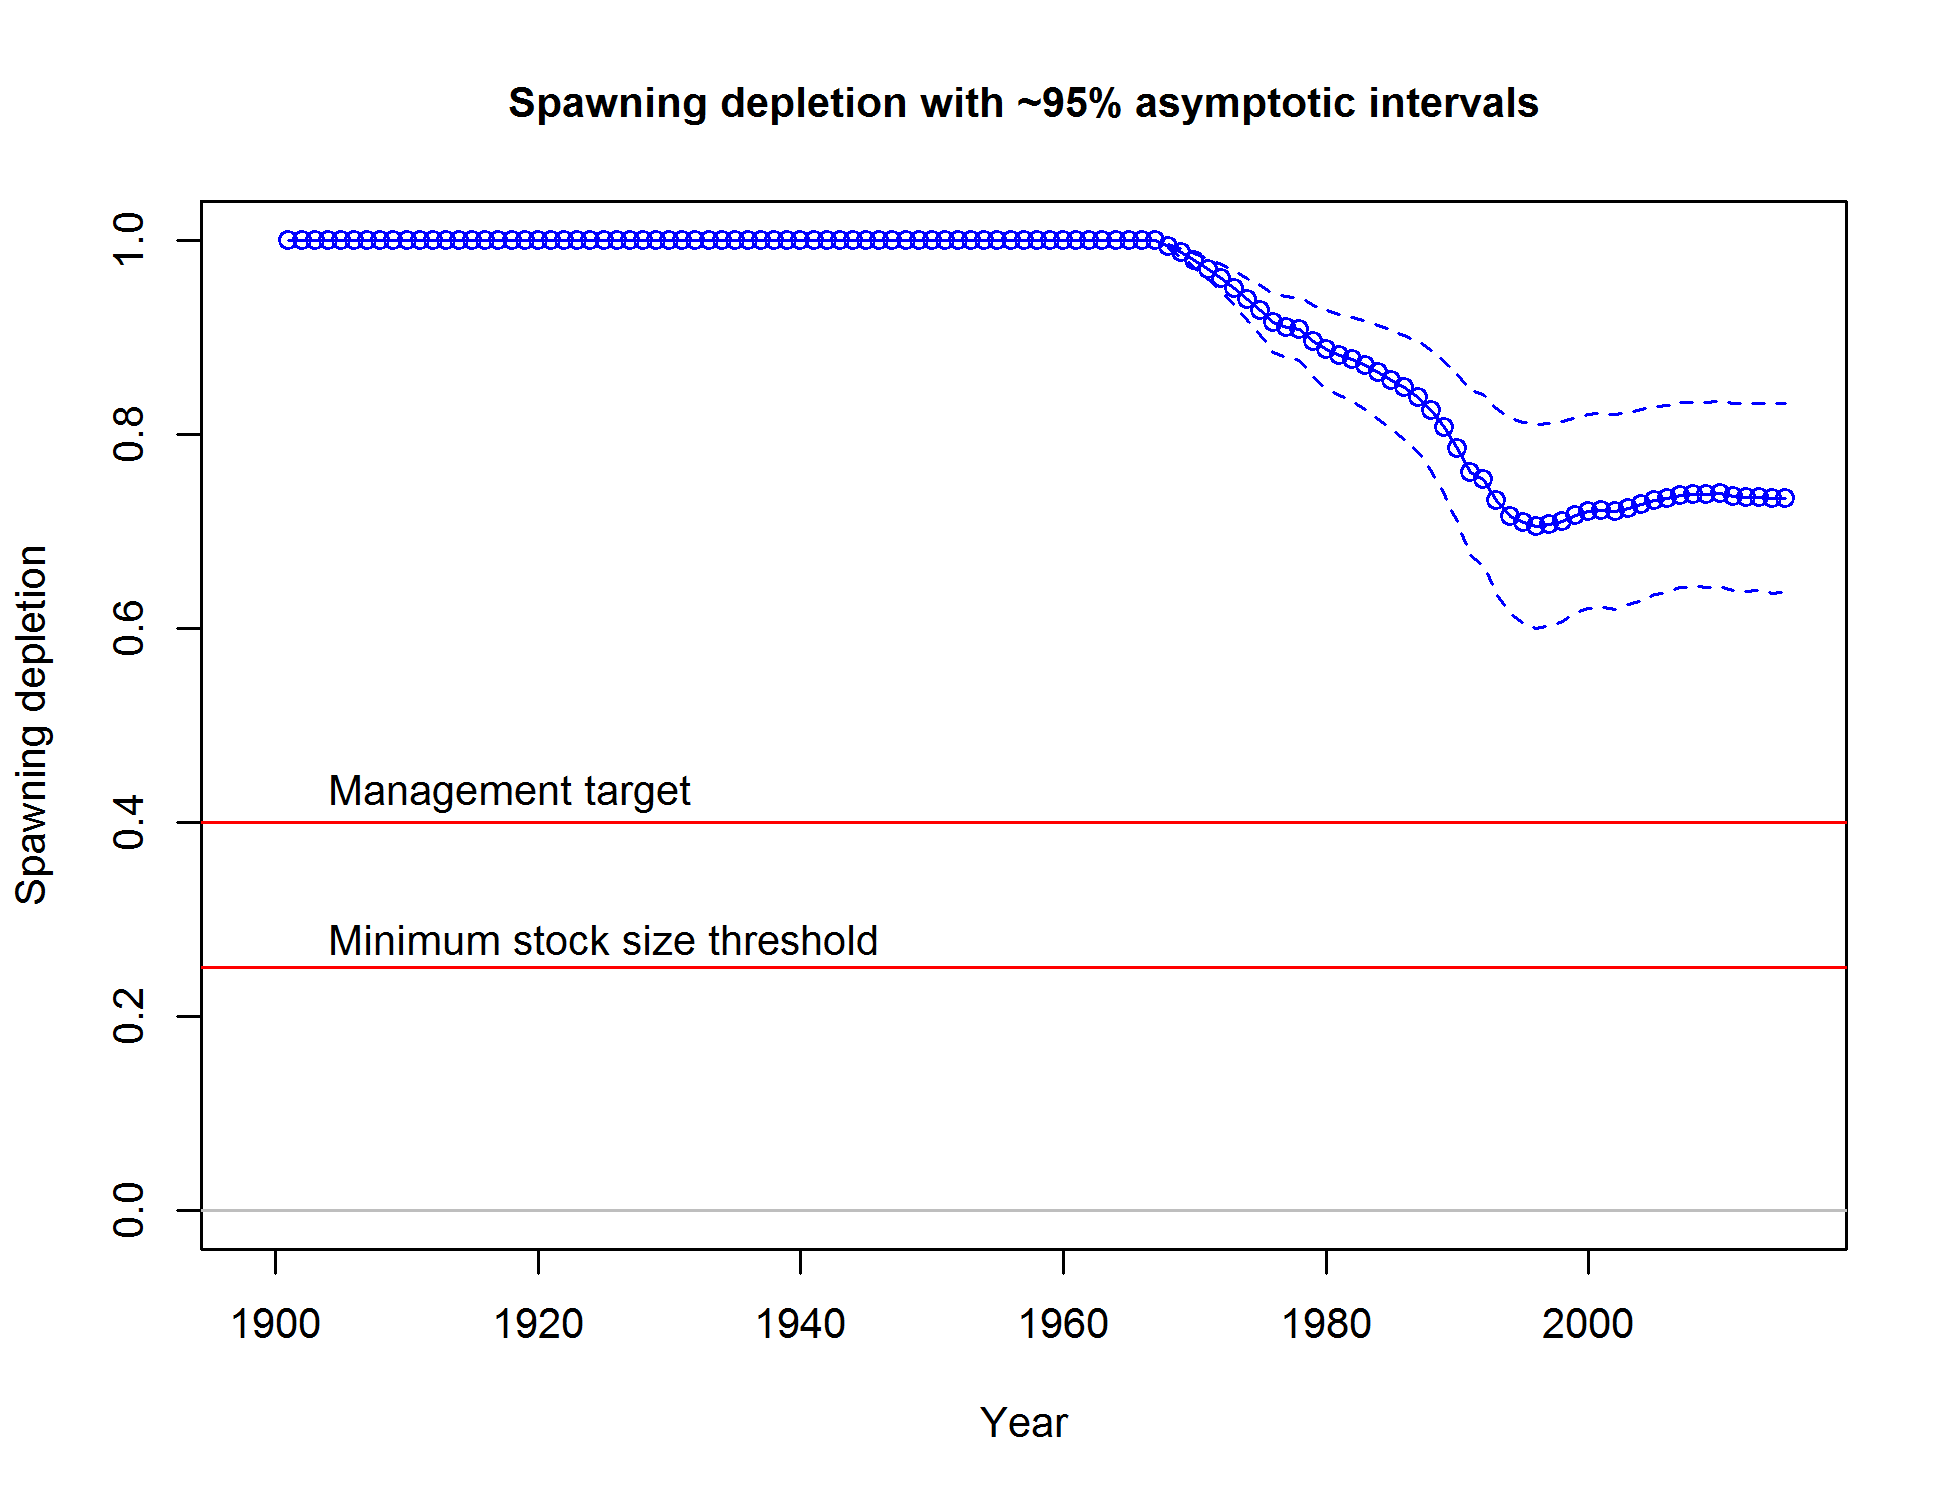
\includegraphics[scale = 0.50, trim={0cm 0cm 0cm 1.7cm}, clip]{r4ss/ts9_Spawning_depletion_with_95_asymptotic_intervals_intervals.png}
  \end{center}
\end{frame}


\begin{frame}{Estimated Annual Recruitment}
  \begin{center}
    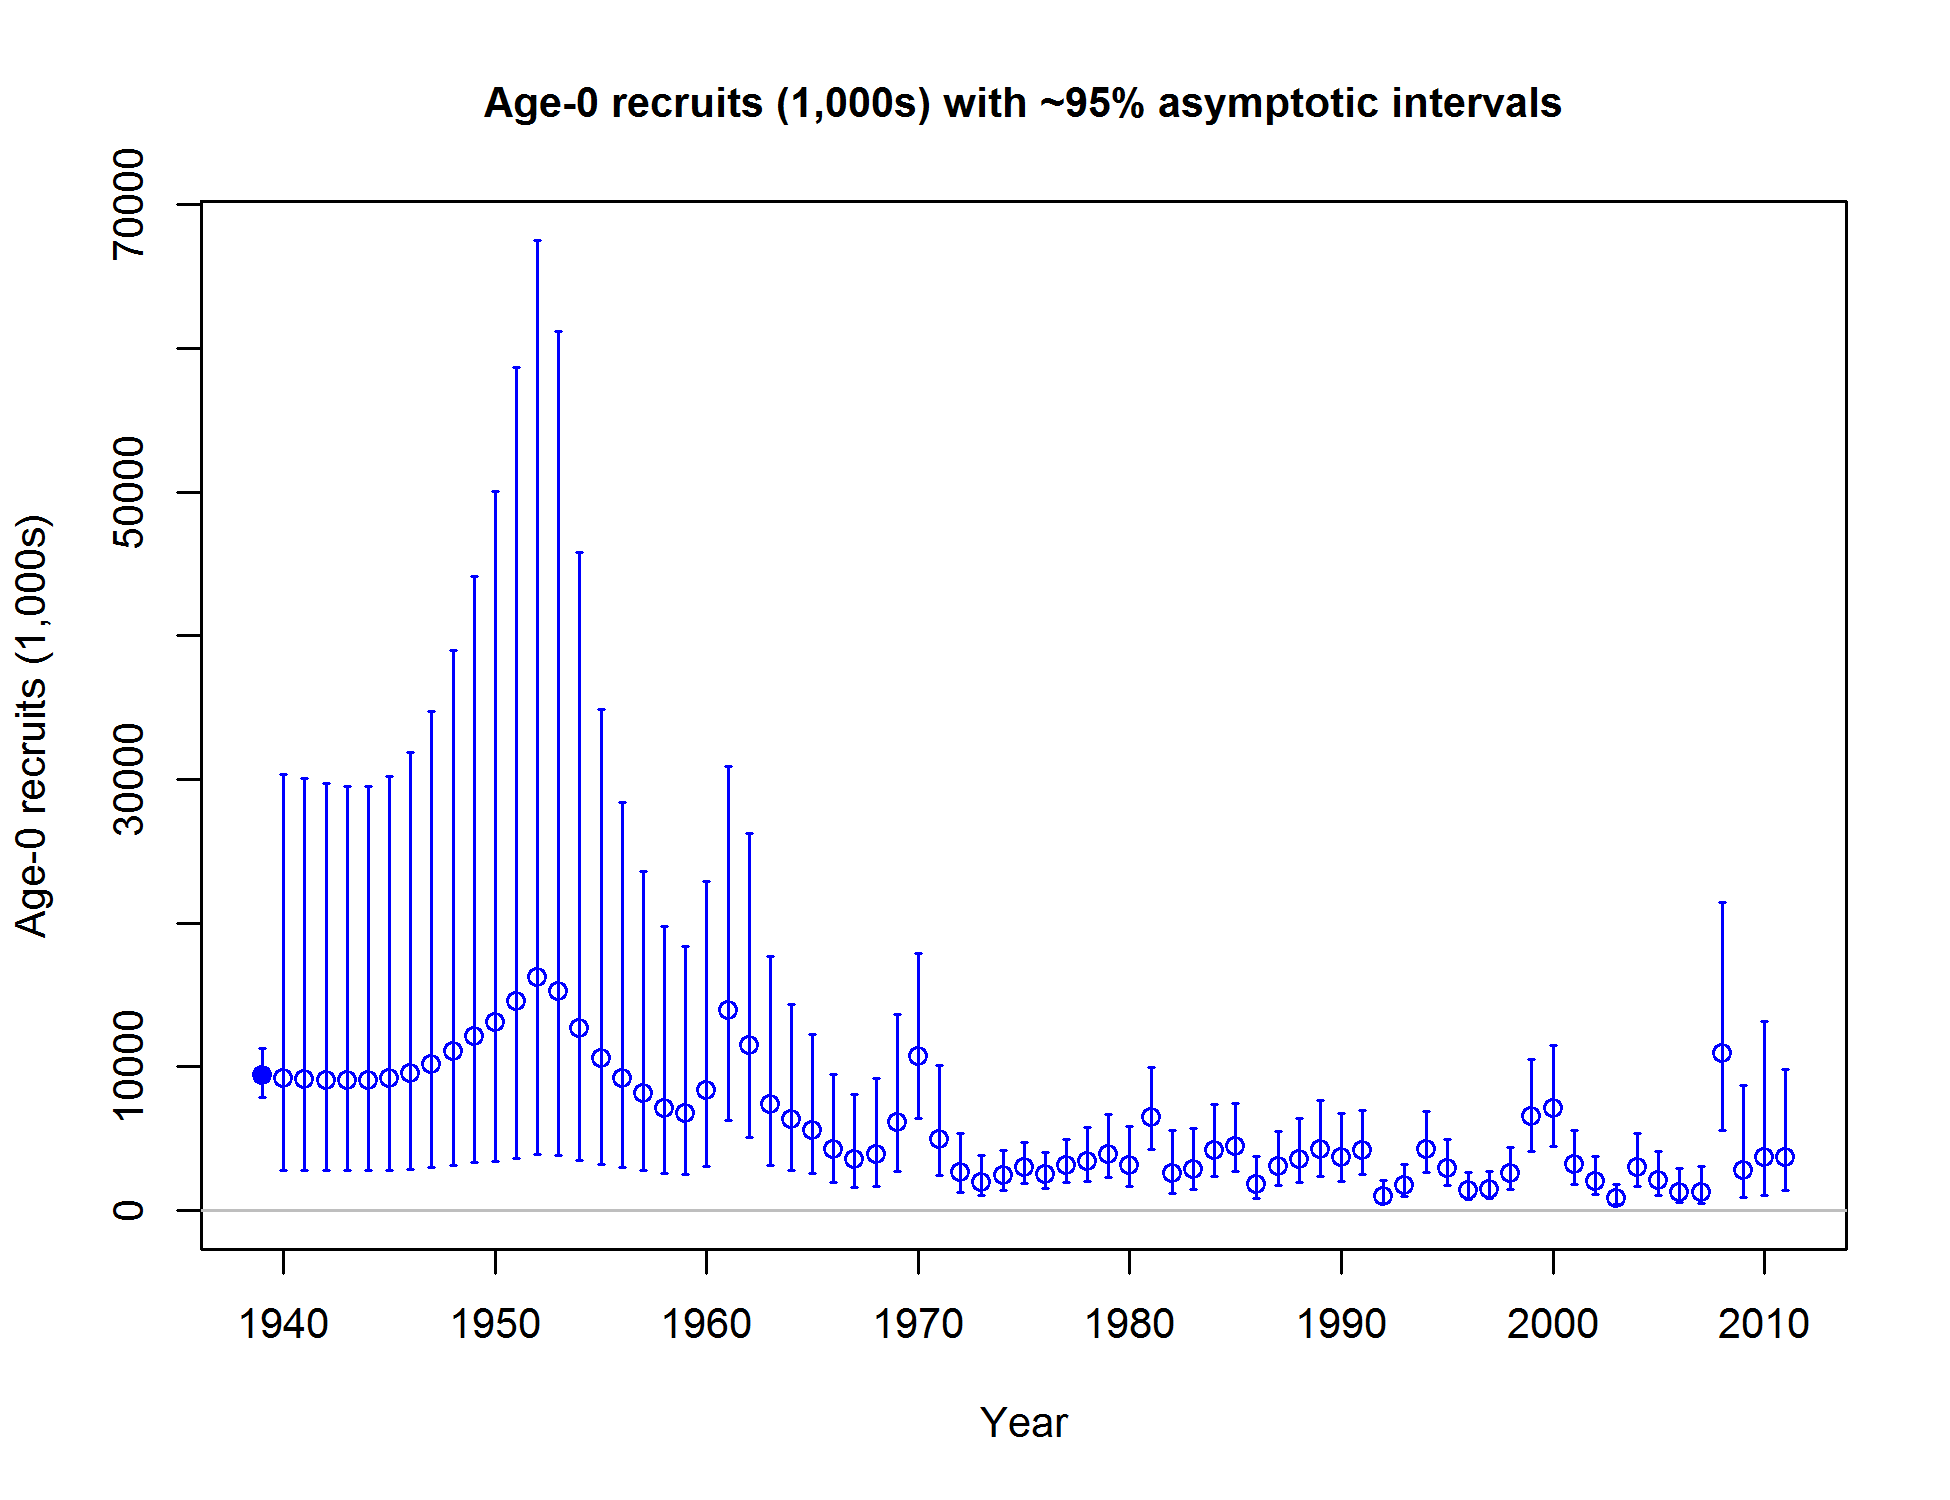
\includegraphics[scale = 0.50, trim={0cm 0cm 0cm 1.7cm}, clip]{r4ss/ts11_Age-0_recruits_(1000s)_with_95_asymptotic_intervals.png}
  \end{center}
\end{frame}

\begin{frame}{Estimated Annual Recruitment Deviations}
  \begin{center}
    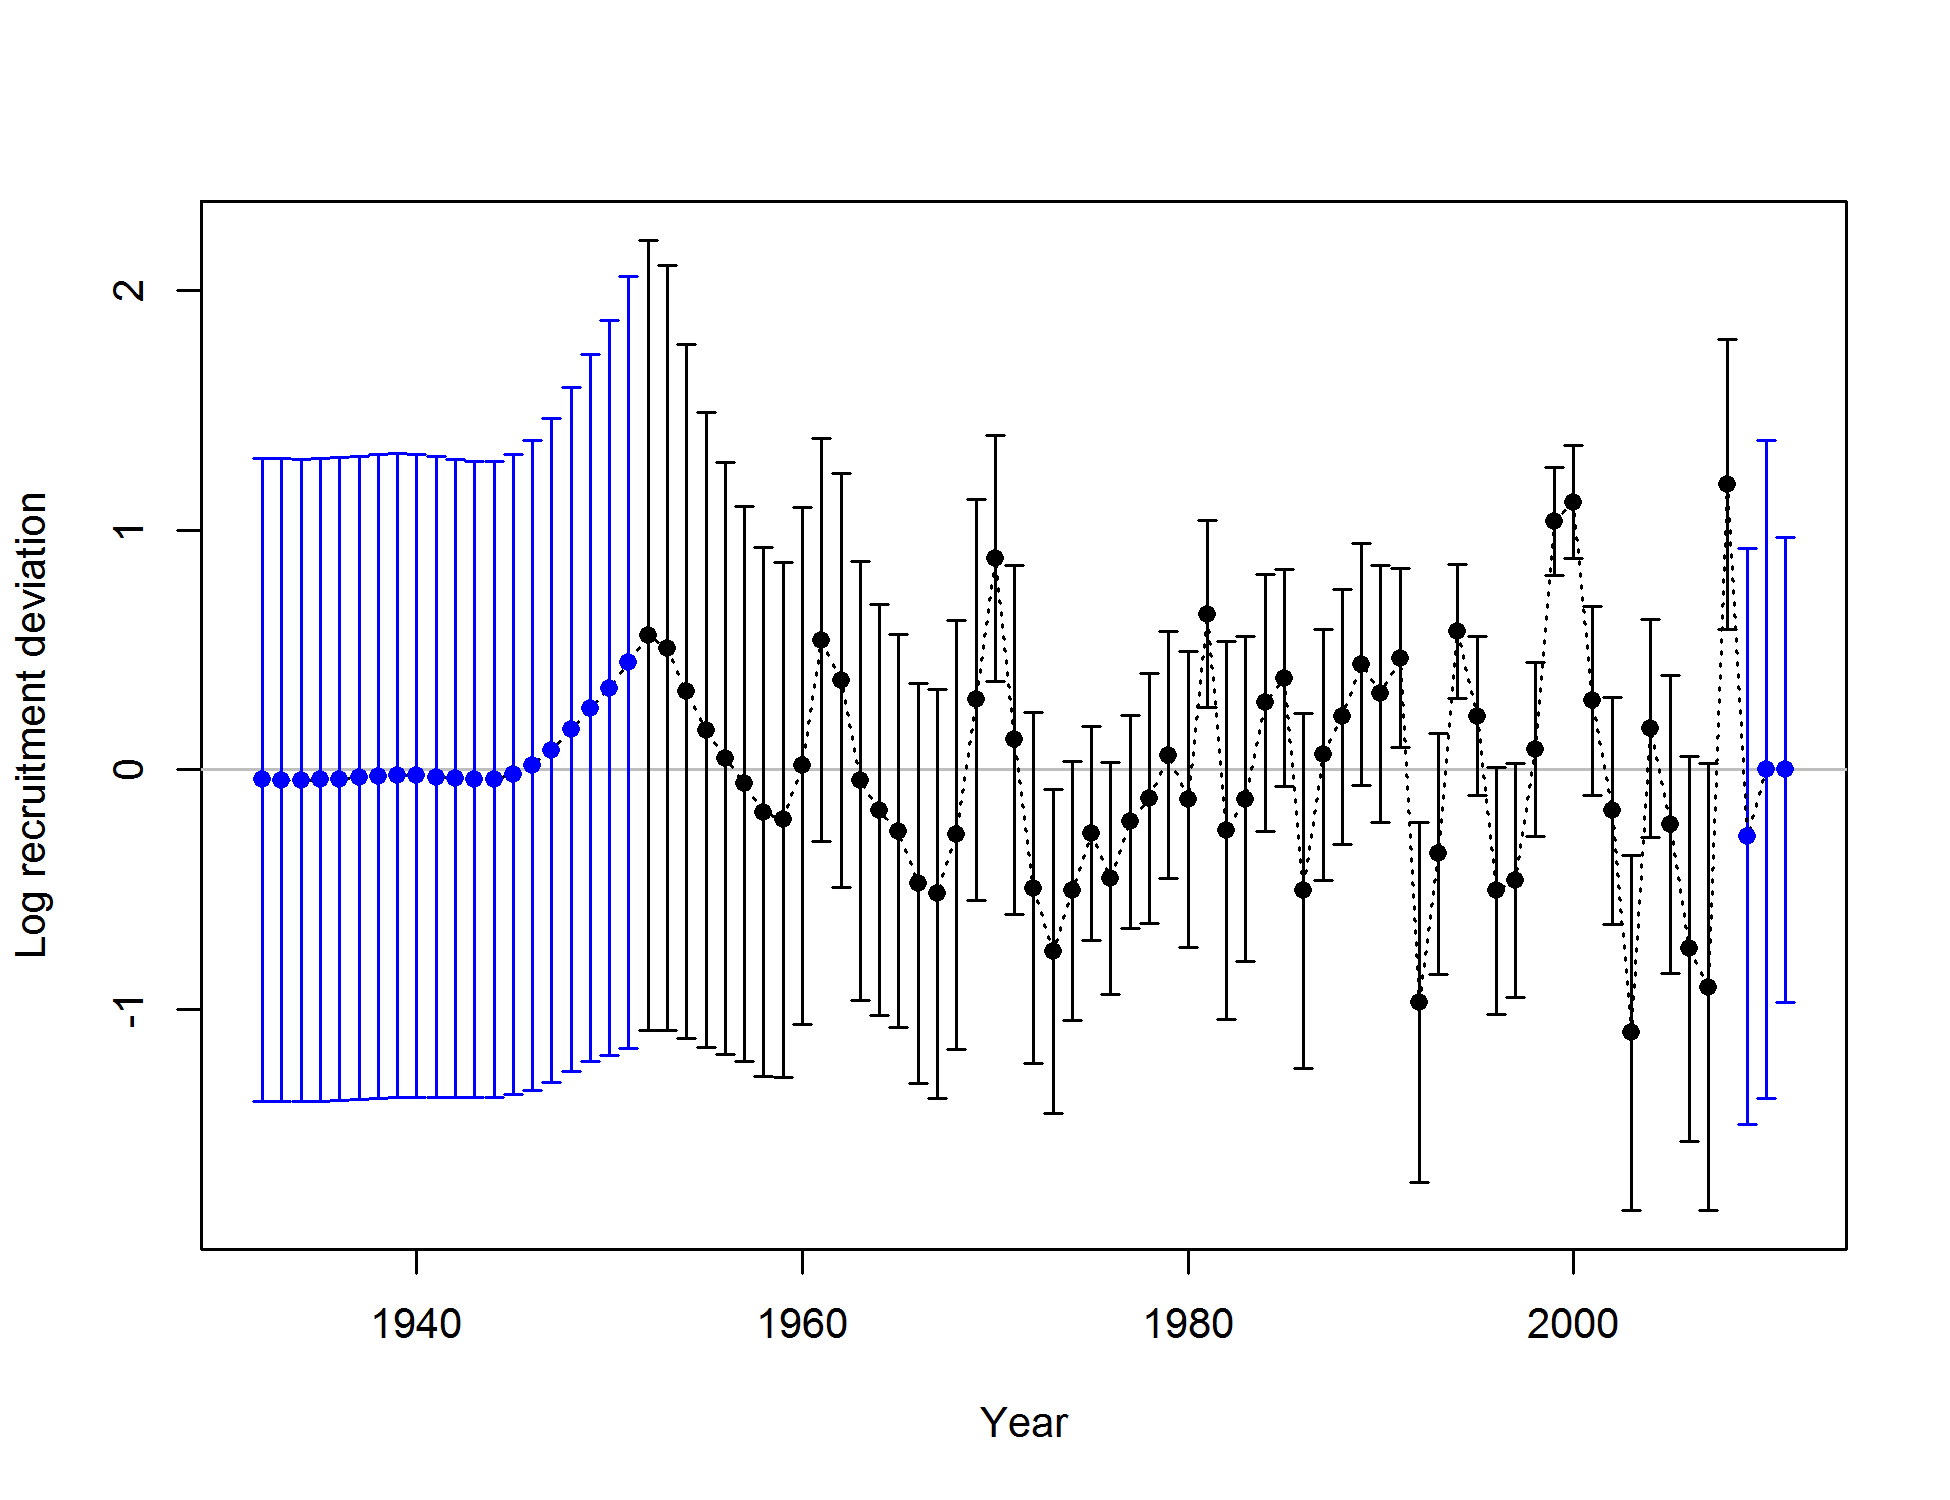
\includegraphics[scale = 0.50, trim={0cm 0cm 0cm 1.7cm}, clip]{r4ss/recdevs2_withbars.png}
  \end{center}
\end{frame}

\subsection{Uncertainties}
\begin{frame}
  \begin{itemize}
    \item Steepness - fixed at 0.50 within the base model.  Likelihood profile over steepness indicates no information in data concerning steepness.  Fixing the value at the steepness prior value of 0.718 results in stock status 97\% of unfished.
    \item Natural Mortality - fixed at 0.054 for males and females, the mean of the prior when maximum age is 100.  Likelihood profile relatively flat around the prior.
    \item Recruitment in 2008 and 2013 - The 2008 data point is relatively certain within the model but an order of magnitude higher than any other year.  Early indications of a strong 2013 recruitment (model is currently underfitting).
  \end{itemize}
\end{frame}

\subsection{Sensitivities}
\begin{frame}
  figures
\end{frame}



%------------------------------------------------------------------------------------
\section{Biology}

%------------------------------------------------------------------------------------
\subsection{Overview}
\begin{frame}{Pacific ocean perch (\textit{Sebastes alutus})}
\begin{columns}
  \begin{column}{0.5\textwidth}
      \begin{itemize}
        \item Distributed from  Alaska Aleutian Islands to Northern California
        \item Typically 200 - 400 meters during summer months
        \item Semi-demersal and can be pelagic
        \item Both sexes move to deeper water with age
      \end{itemize}
  \end{column}
  
  \begin{column}{0.5\textwidth}
    \includegraphics[height = 1in]{C:/Users/Chantel.Wetzel/Documents/GitHub/POP_2017/Sebastes_alutus.png}
    %\includegraphics[height = 1in]{Sebastes_alutus.png}
    \begin{itemize}
        \item Female move to deeper waters post-spawning during winter months and return inshore in spring.
      \end{itemize}
  \end{column}
\end{columns}
\end{frame}


\subsection{Maturity}
\begin{frame}{Maturity}
\begin{columns}
  \begin{column}{0.5\textwidth}
      Functional maturity-at-length
      \begin{itemize}
        \item Categorized mature and immature fish based on the proportion of vitellogenin in the cytoplasm and atretic celss
        \item 50\% maturity is at larger lengths vs. biological maturity
        \item functional 50\% = 32.1 cm vs. biological 50\% = 30.1 cm
      \end{itemize}
  \end{column}
  
  \begin{column}{0.5\textwidth}
  \begin{center}
    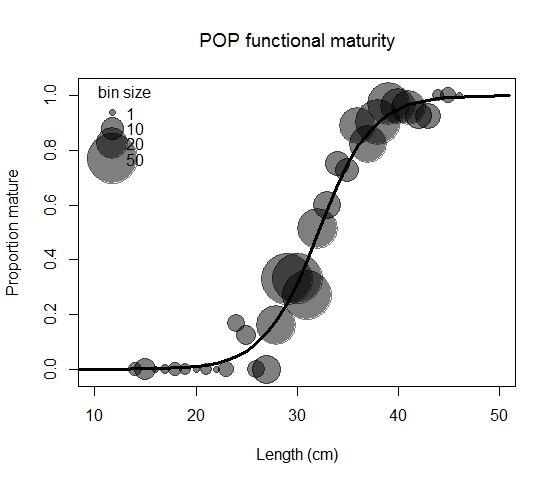
\includegraphics[height = 2.75in, width = 2.5in]{figures/Functional_Maturity.png}
  \end{center}
  \end{column}
\end{columns}
\end{frame}

\begin{frame}{Maturity Comparison}
  \begin{center}
    %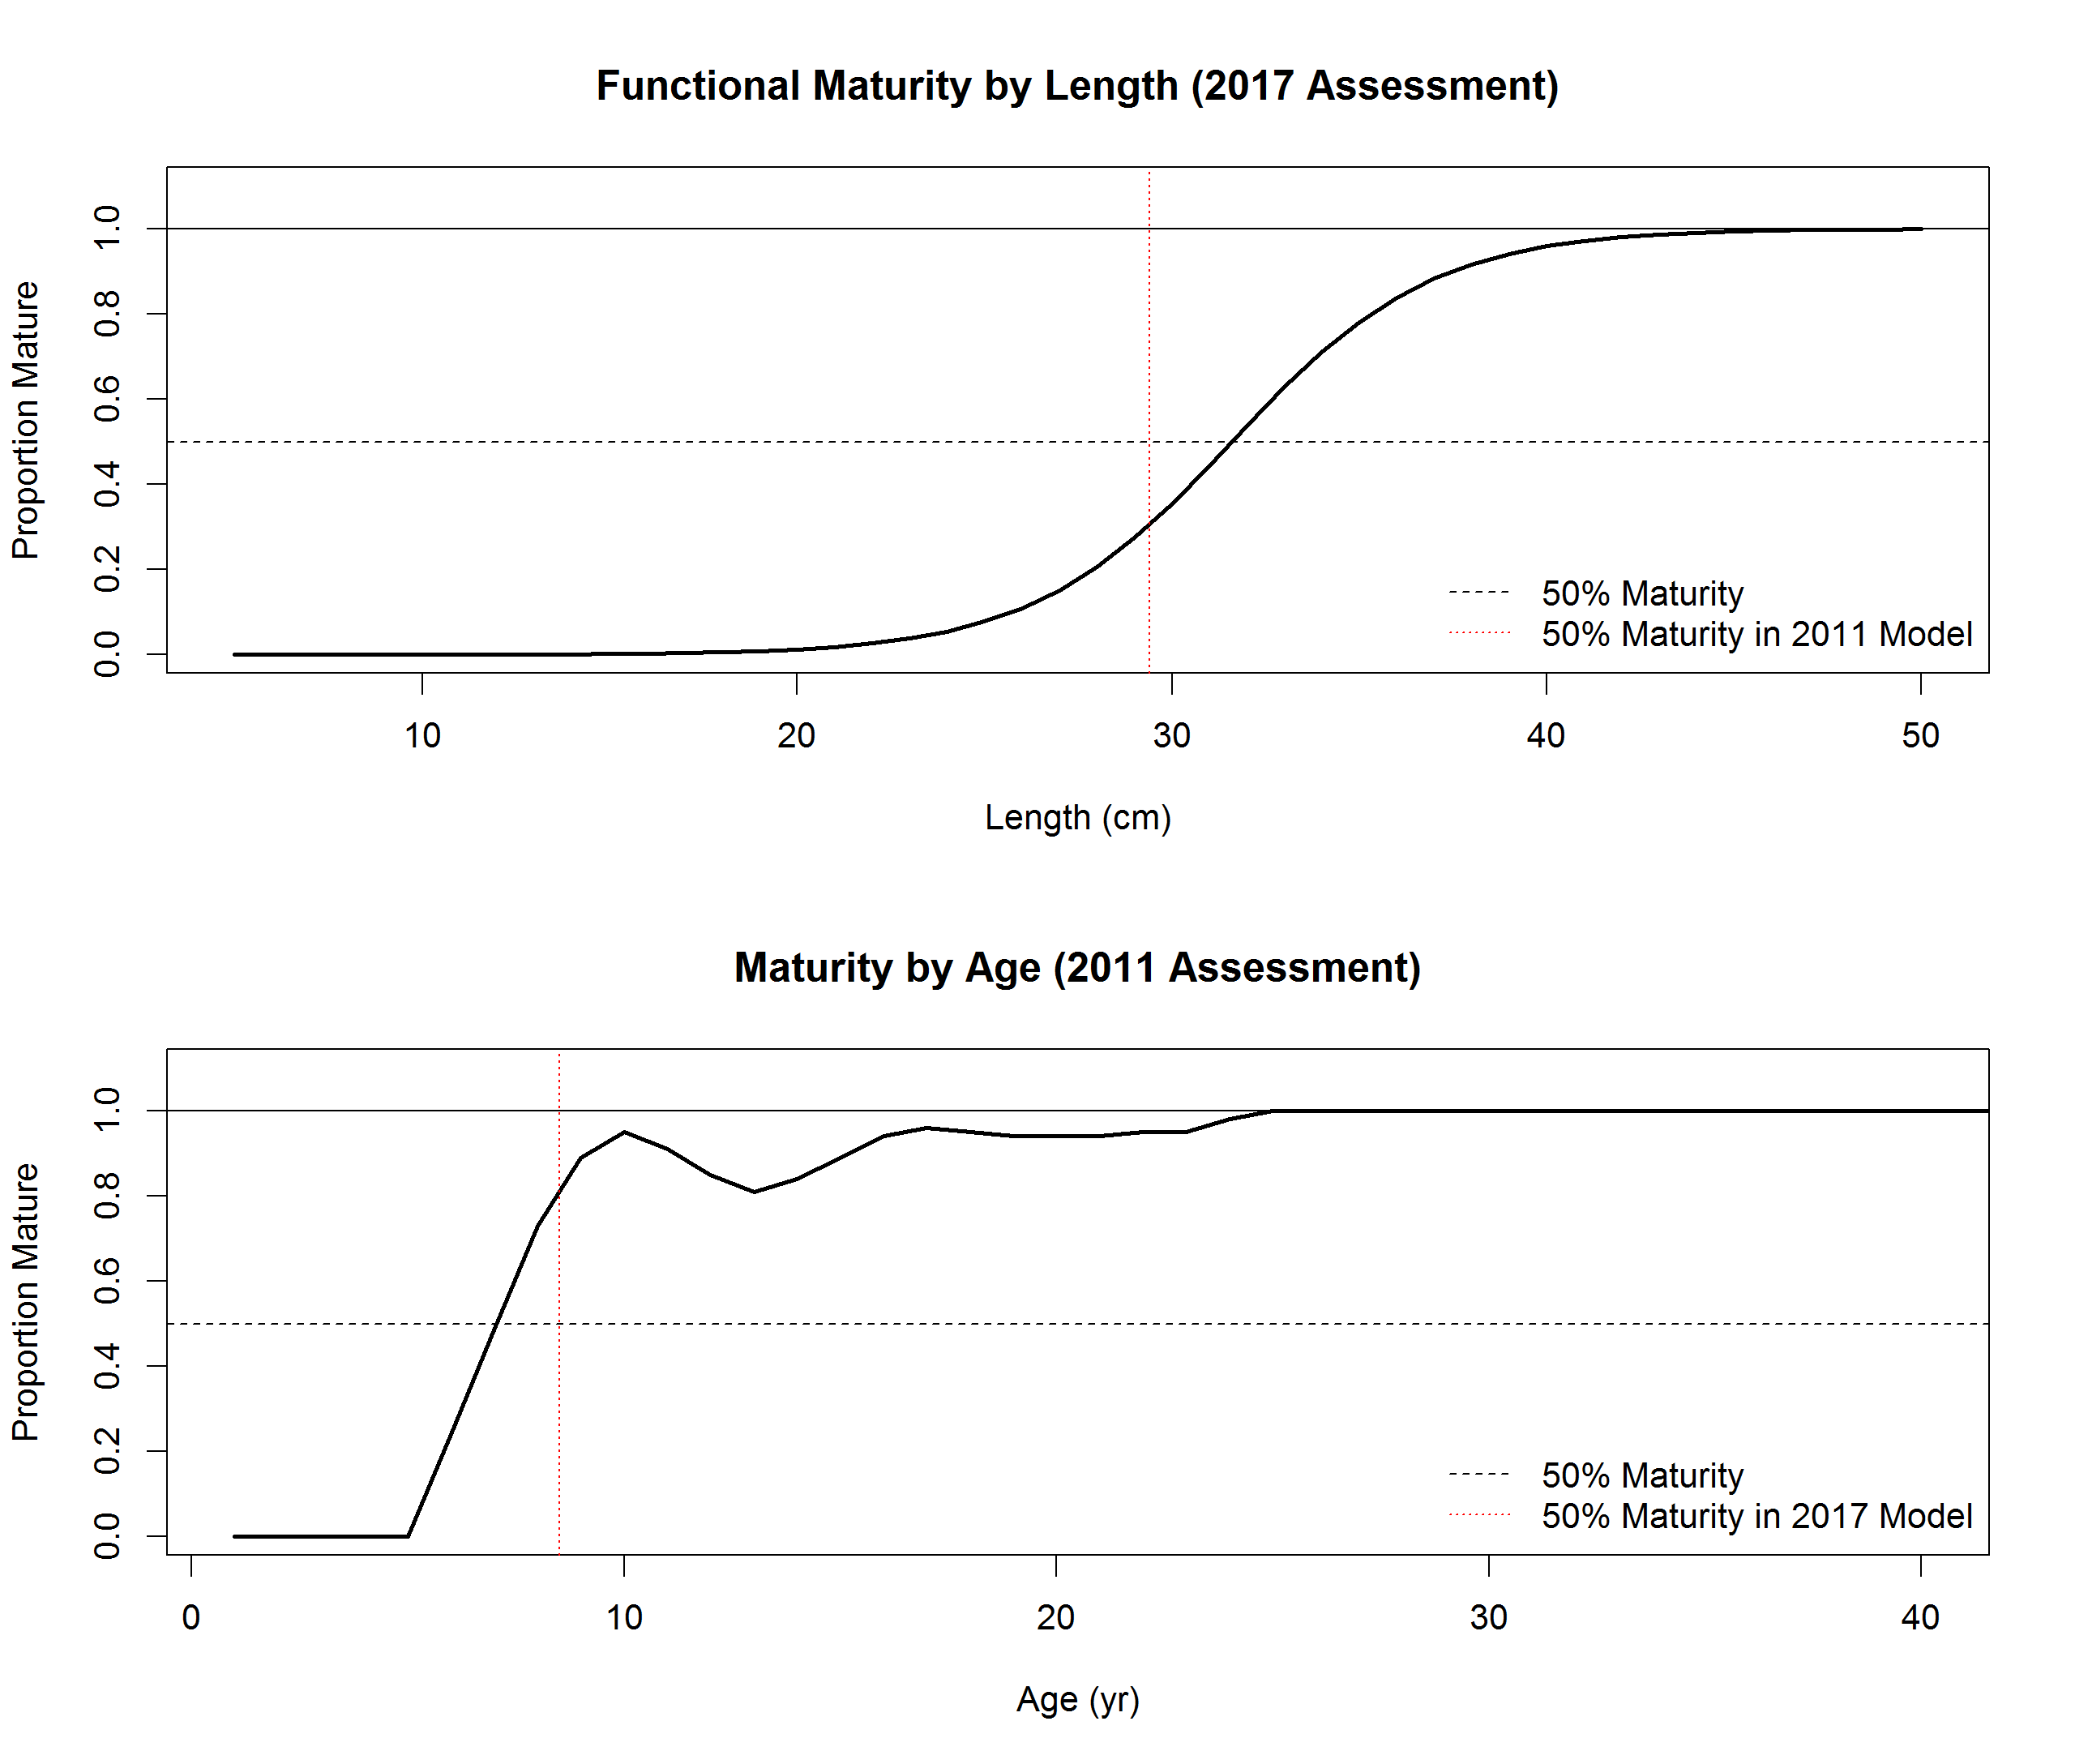
\includegraphics[height = 2.75in, width = 3.5in]{figures/Maturity_Comparison.png}
    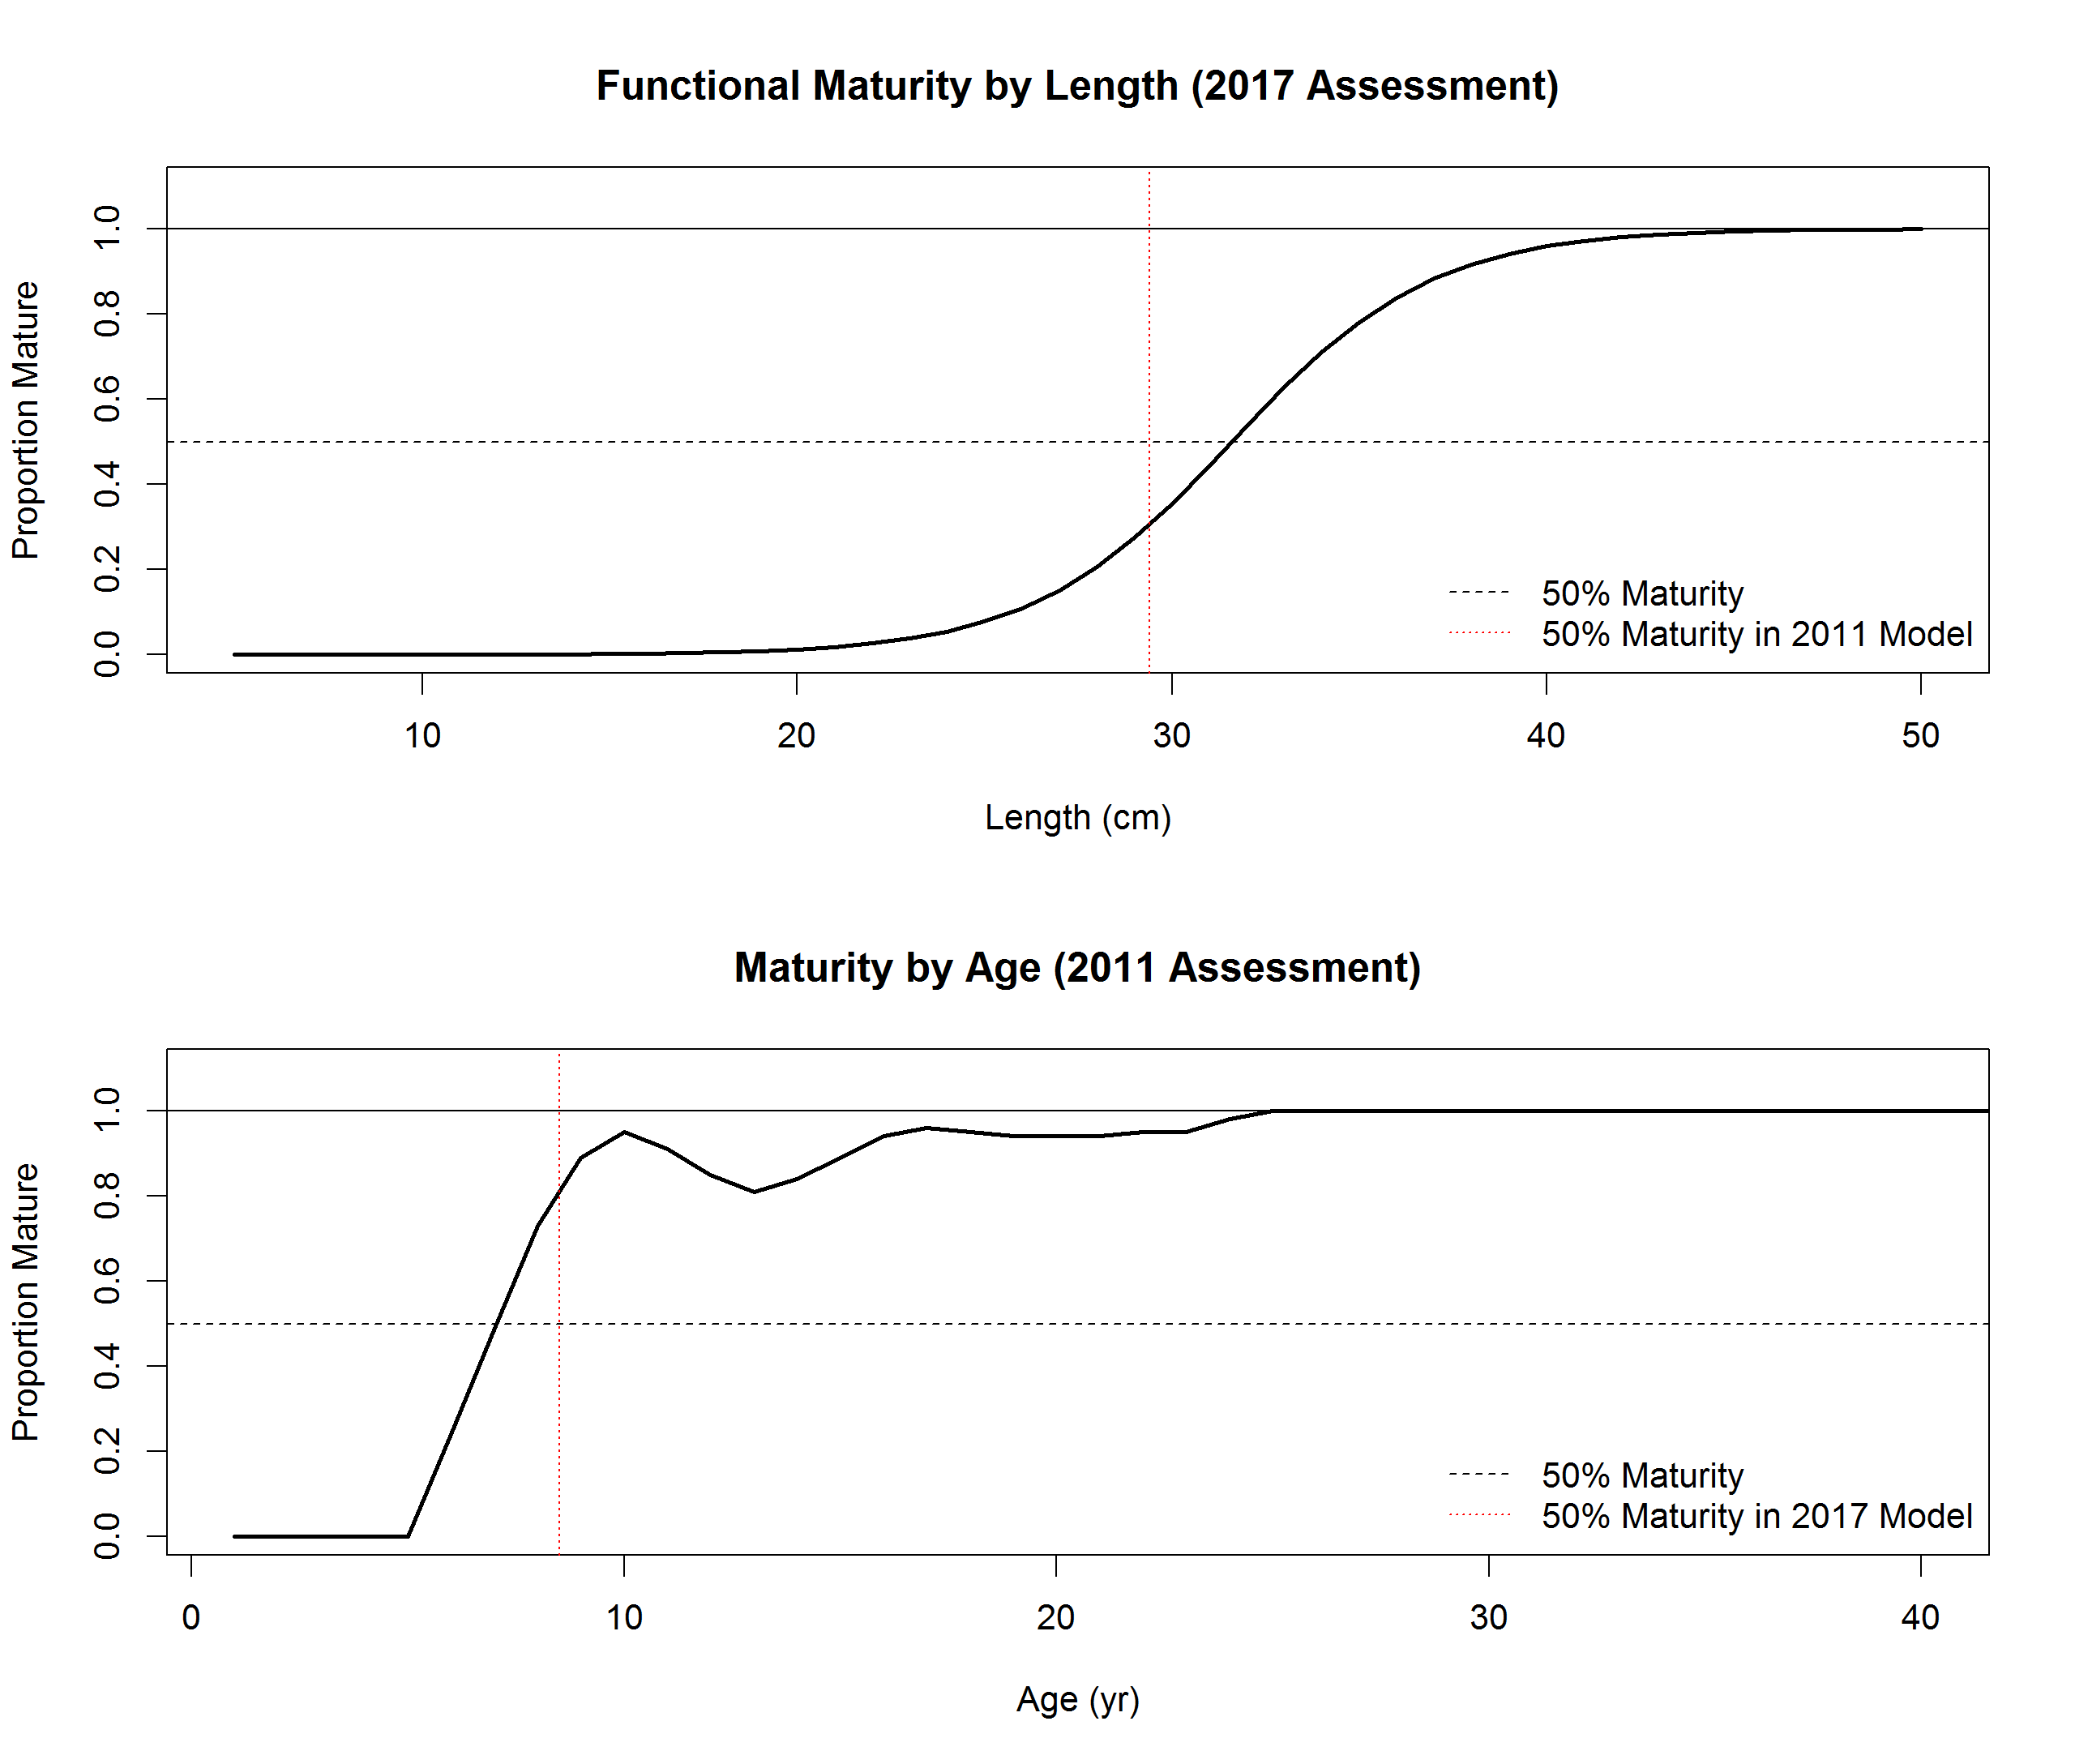
\includegraphics[scale = 0.32]{figures/Maturity_Comparison.png}
  \end{center}
  *Sensitivity assumed maturity shown to not have a large impact on results
\end{frame}

\subsection{Fecundity}
\begin{frame}{Fecundity}
  \begin{center}
    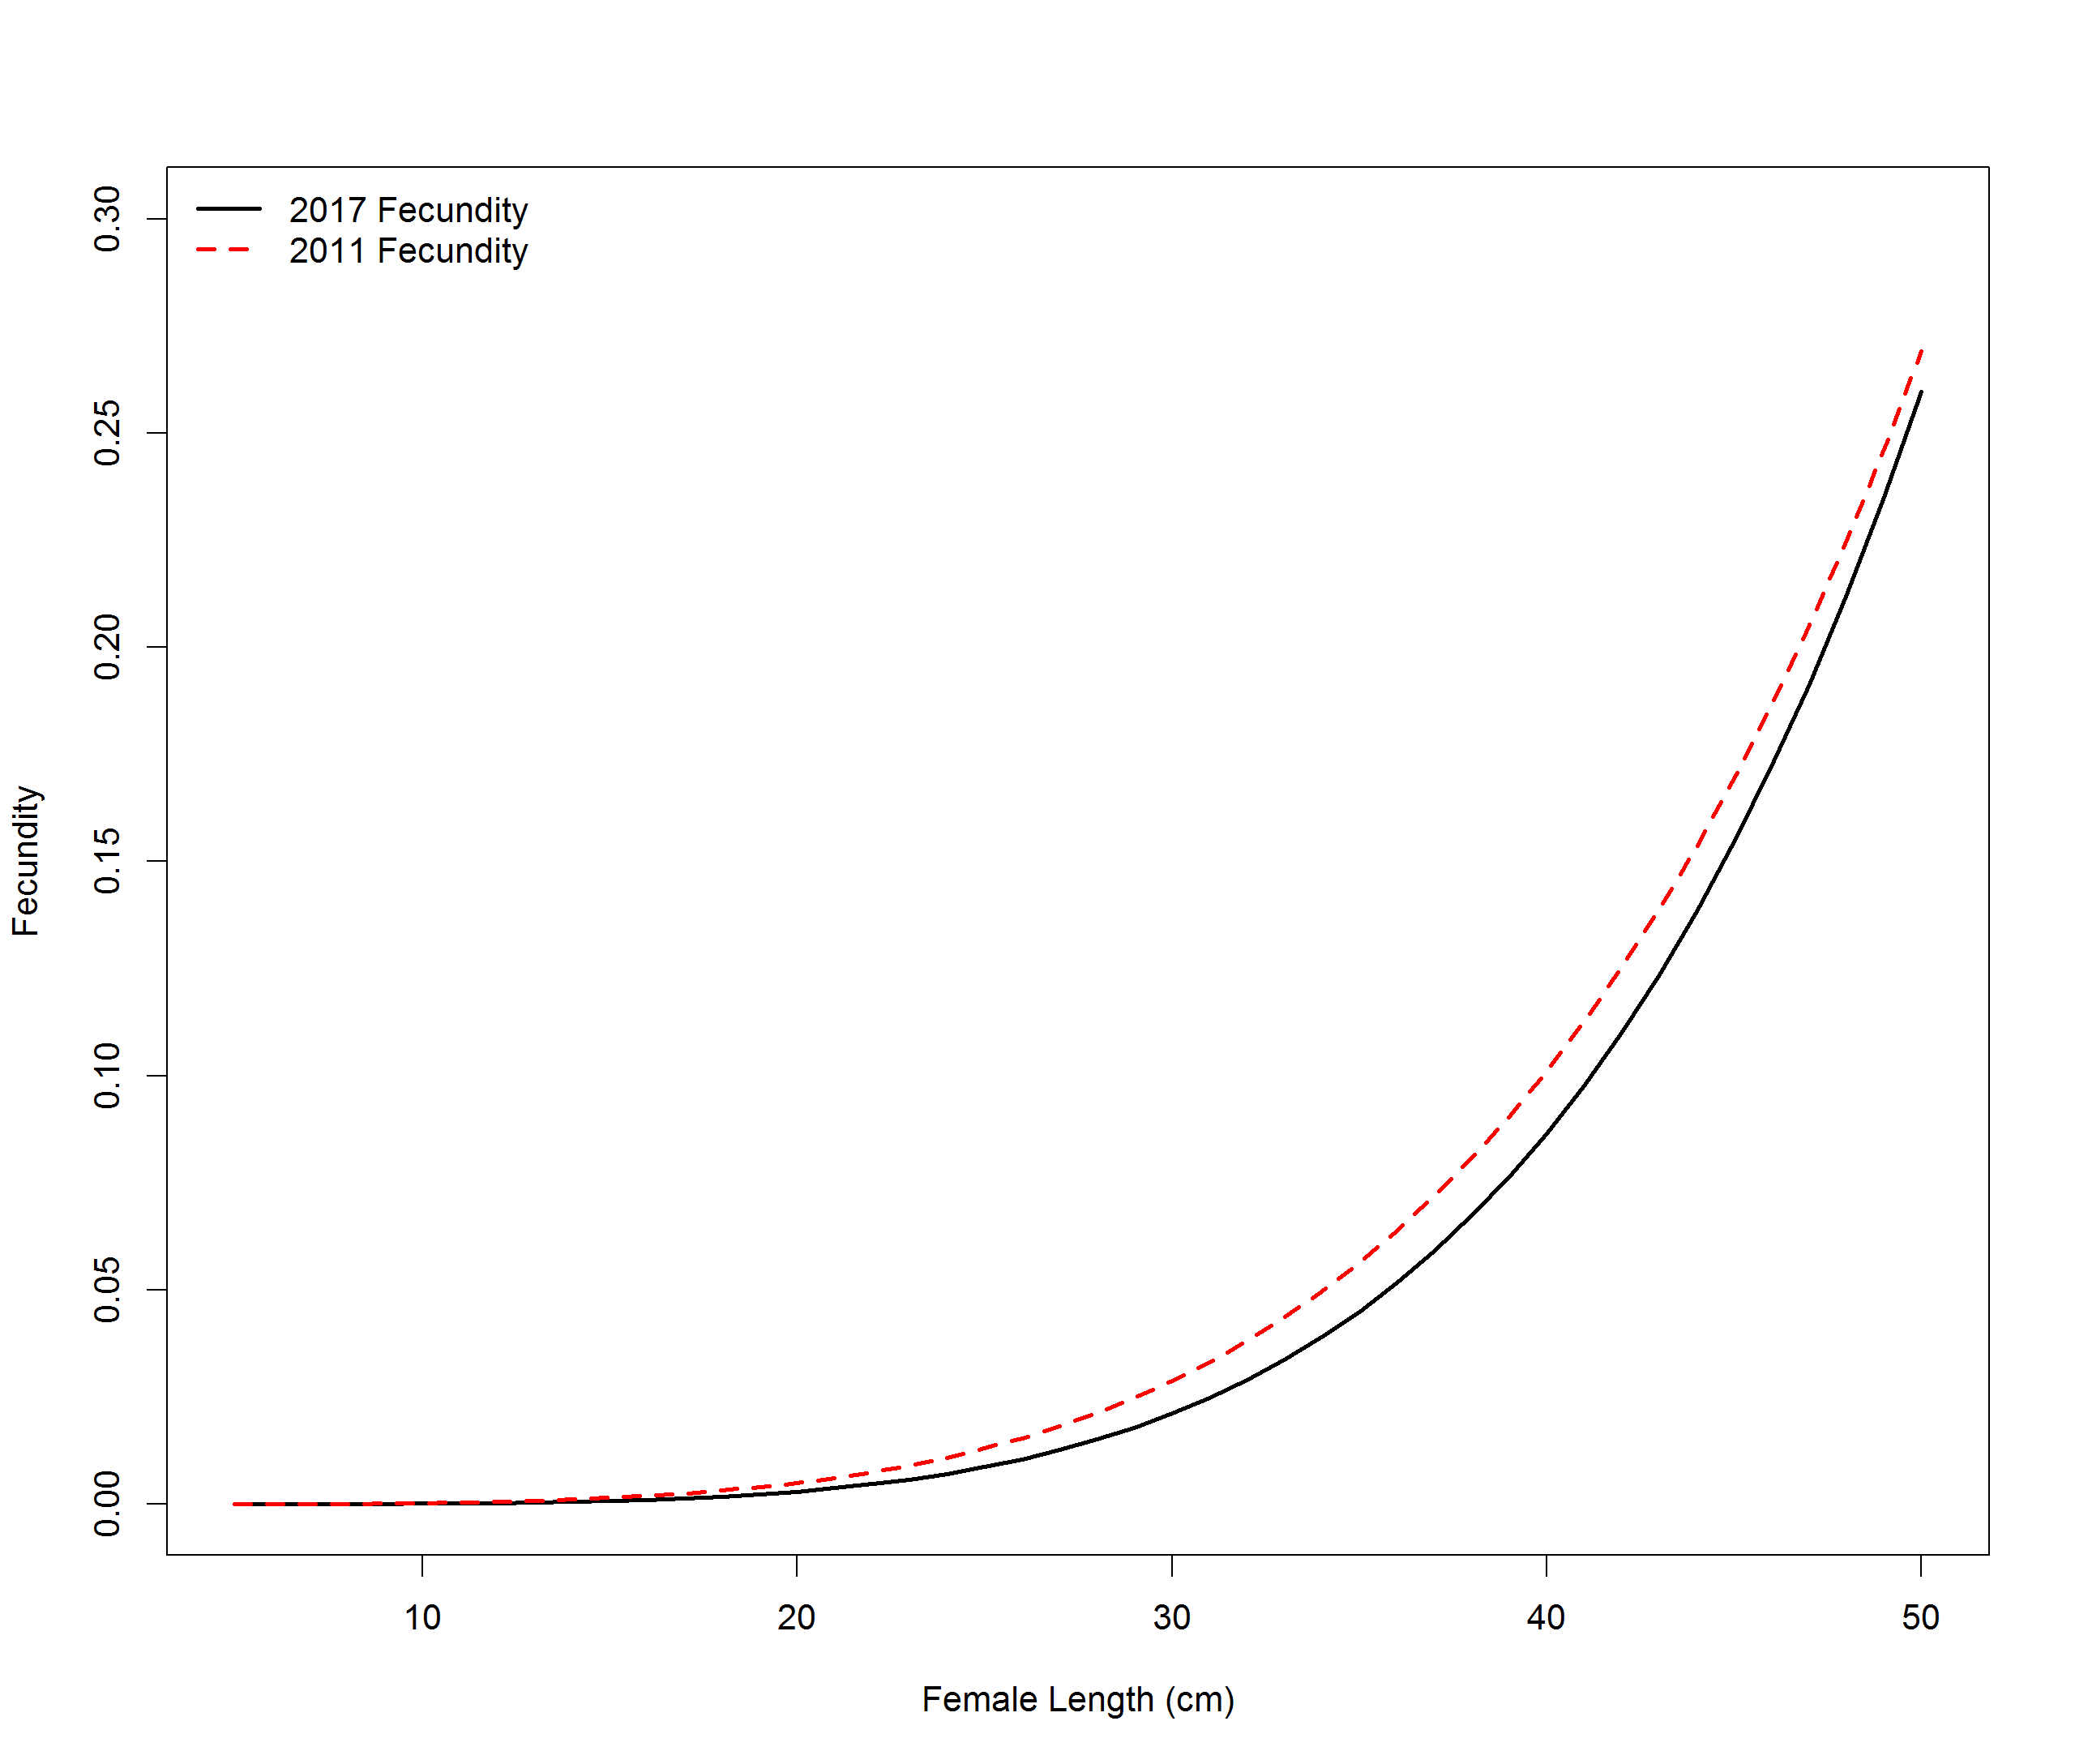
\includegraphics[scale = 0.3, trim={0, 0, 1cm, 1cm}, clip]{figures/Fecundity_Comparison.png}
  \end{center}
  *Sensitivity to assumed fecundity shown to not have a large impact on results
\end{frame}

\subsection{Growth}
\begin{frame}{Weight-at-length}
  \begin{center}
    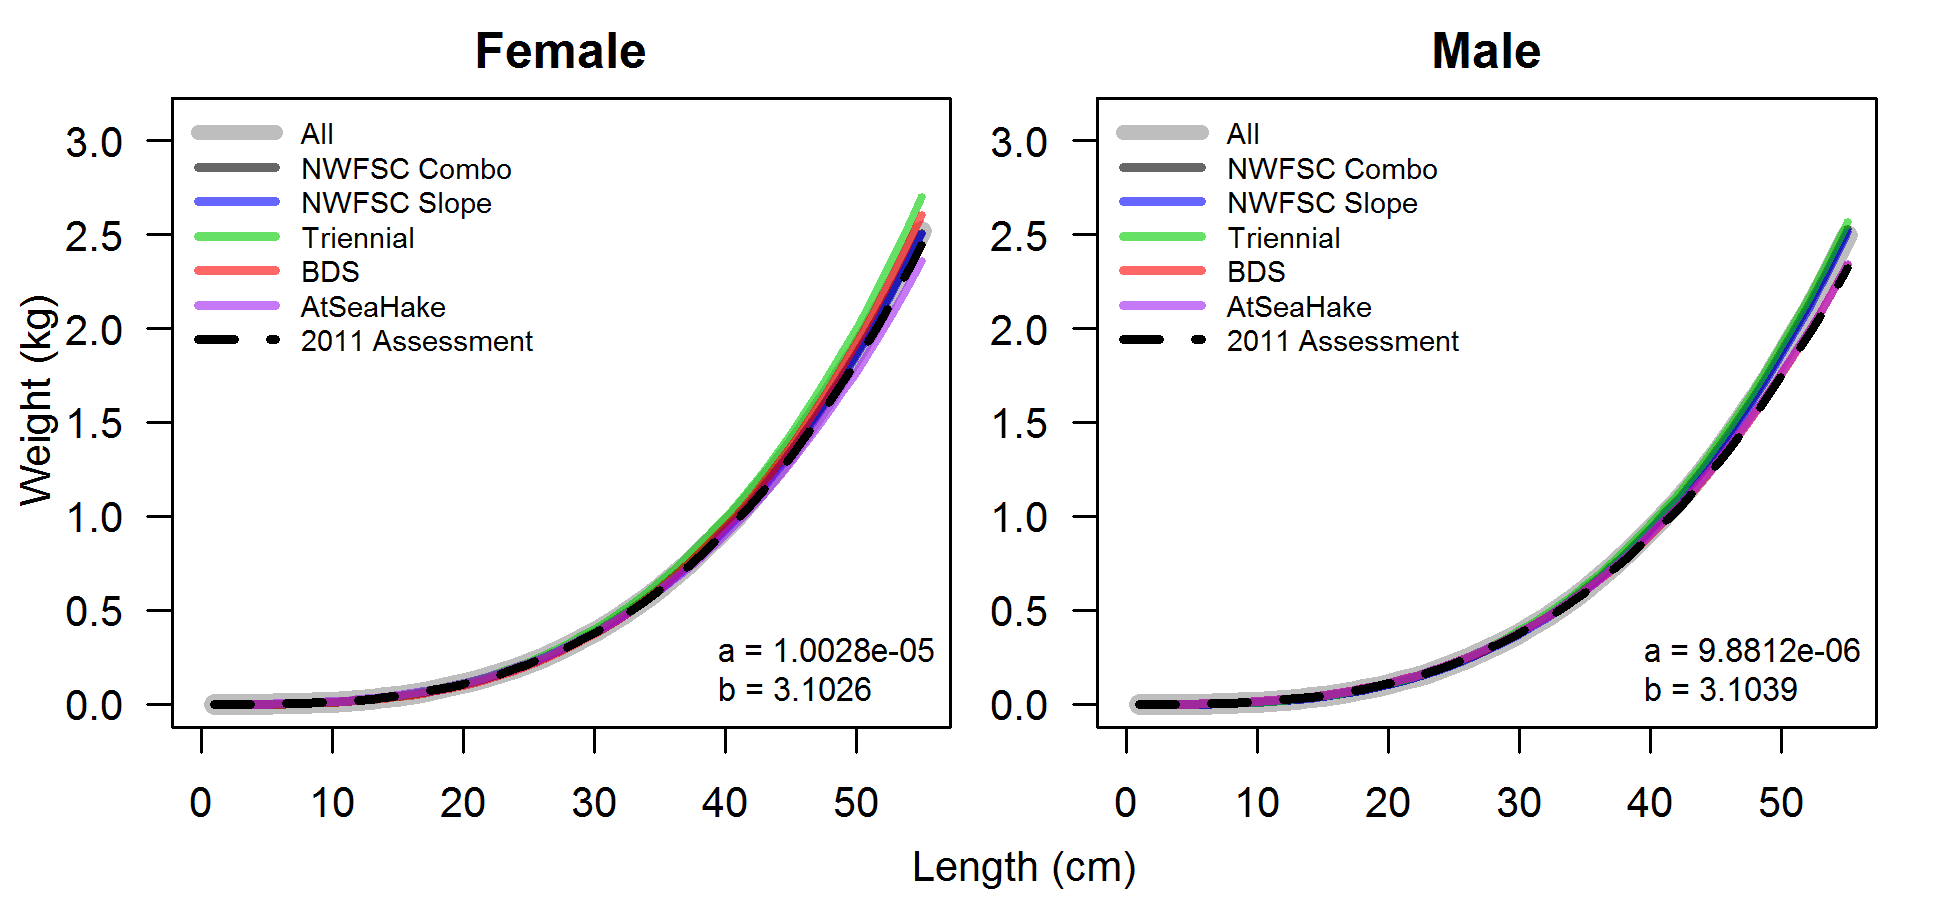
\includegraphics[scale = 0.75]{figures/weightAtLengthPred.png}
  \end{center}
\end{frame}

\begin{frame}{Length-at-age}
  \begin{center}
  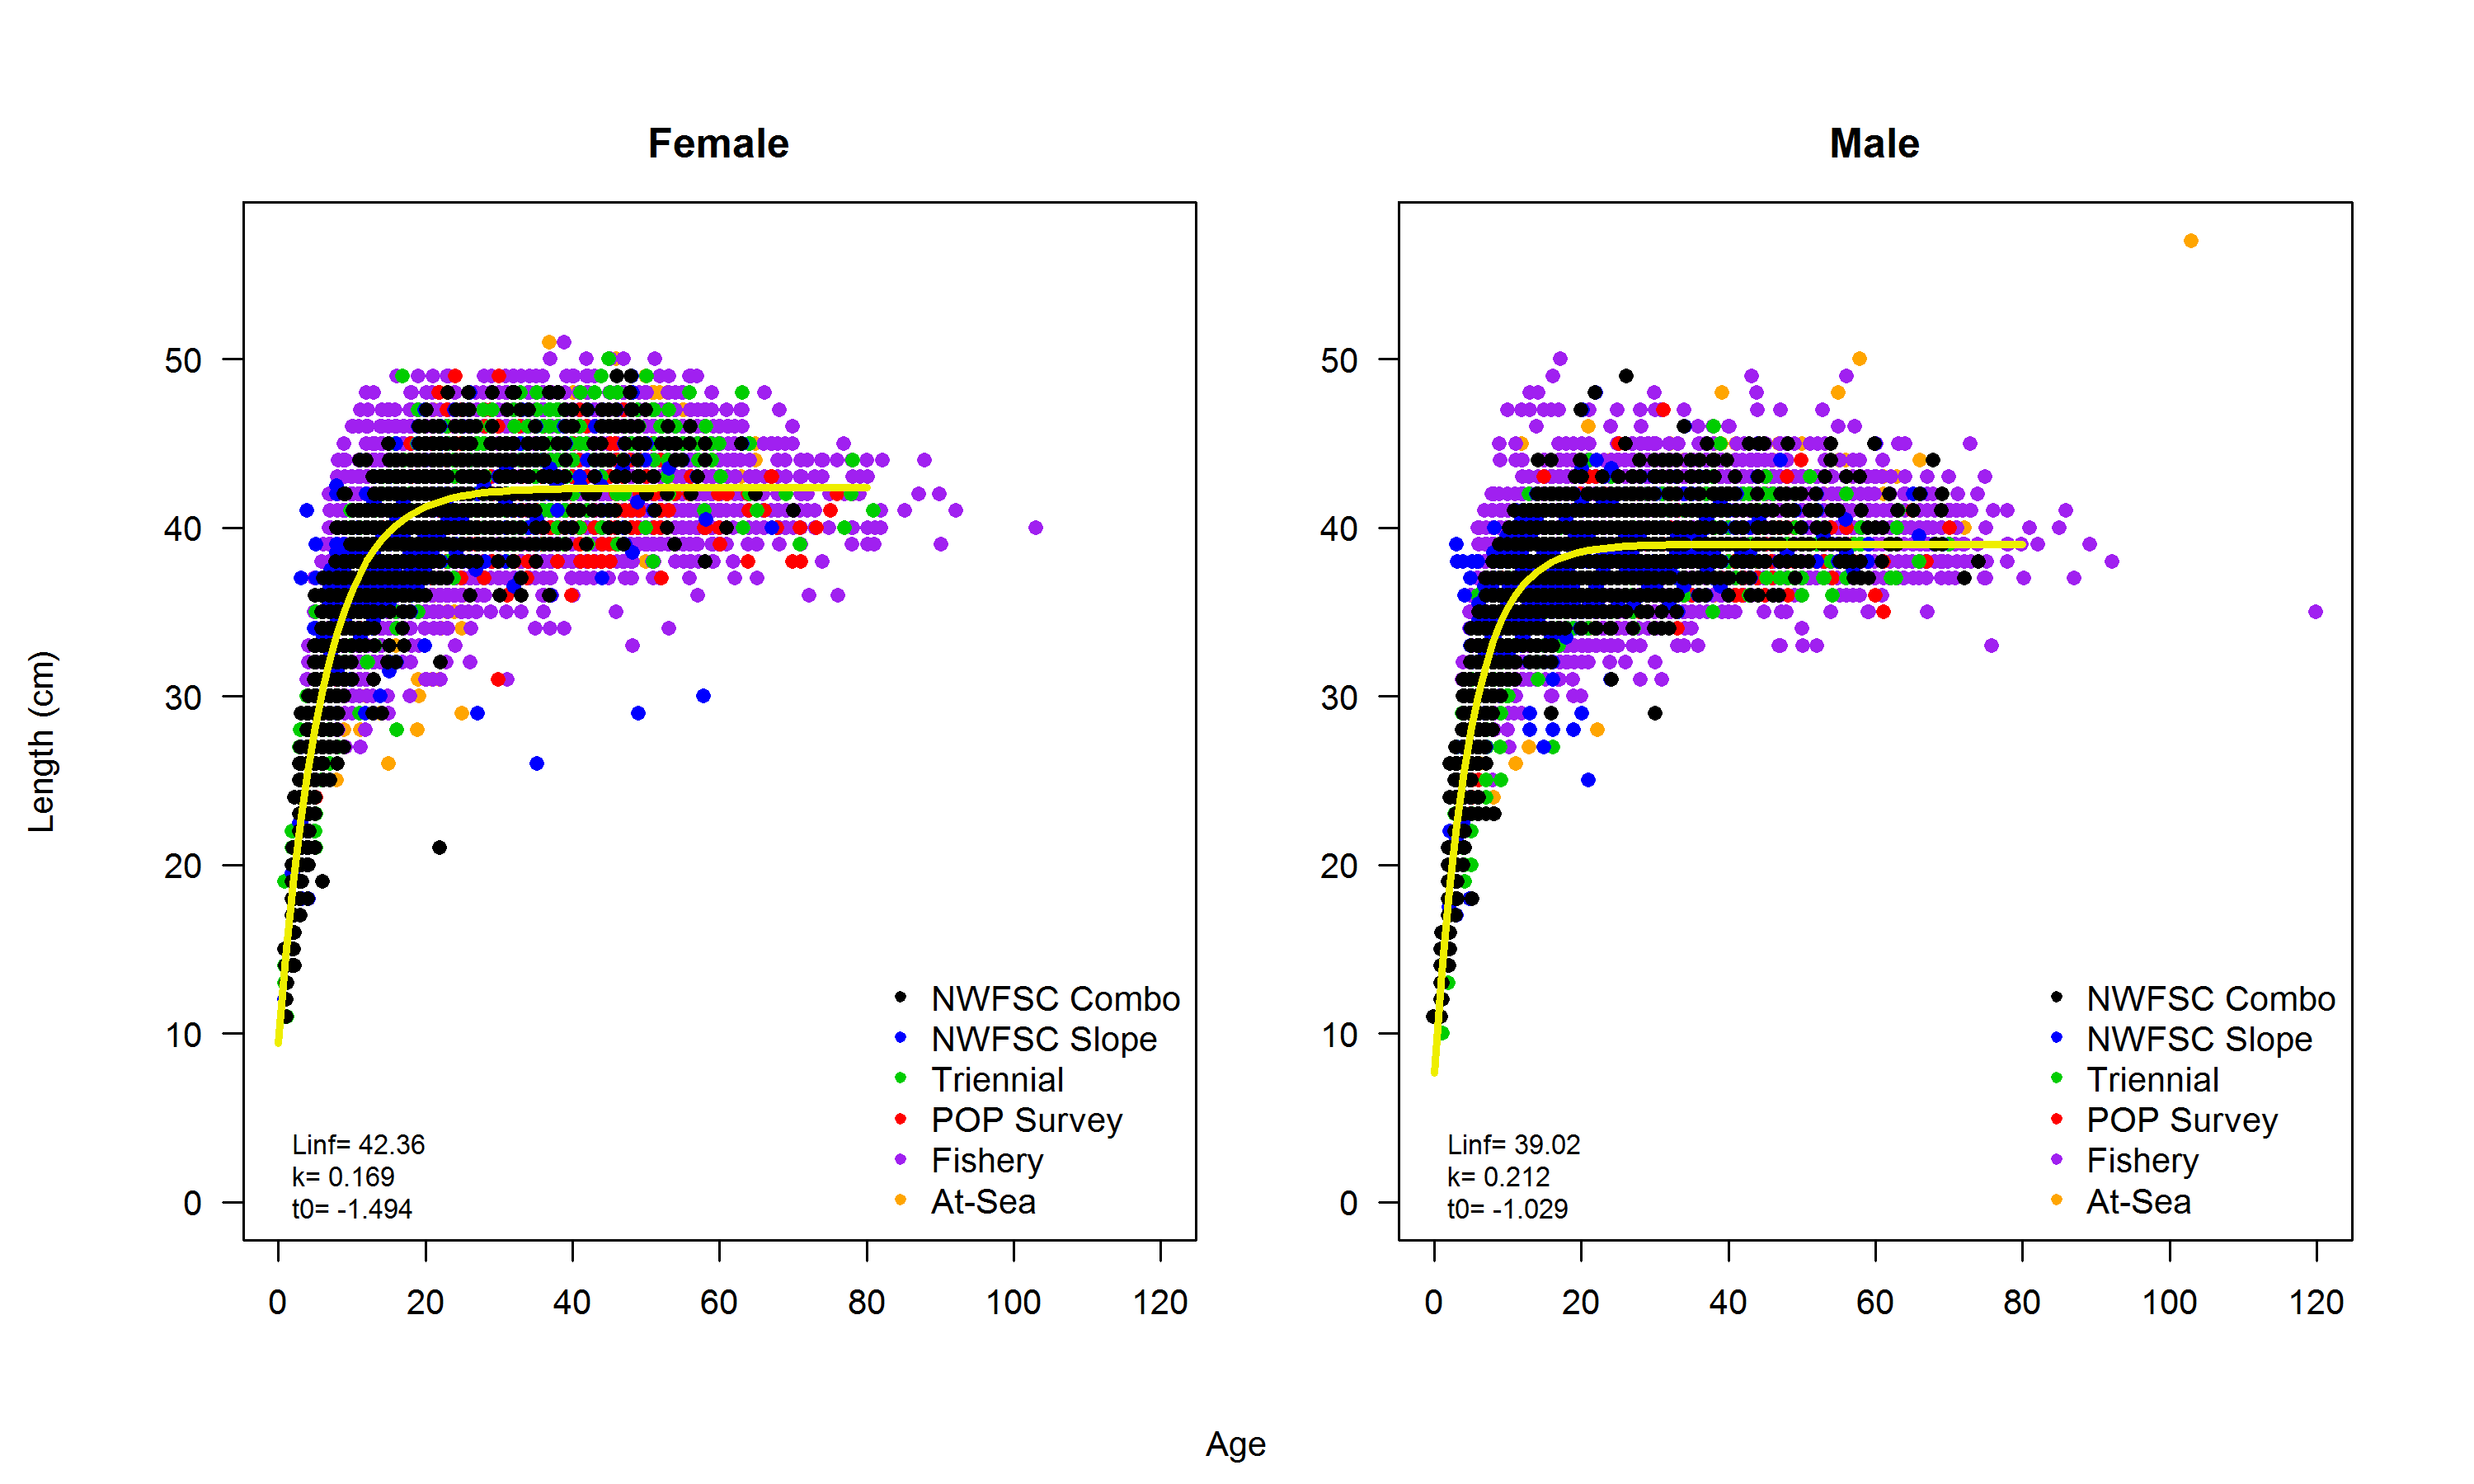
\includegraphics[scale = 0.5]{figures/LengthAgeAll_2.png}
  \end{center}
\end{frame}


\begin{frame}{Observed Ages}
  \begin{columns}
    \begin{column}{0.35\textwidth}
      \begin{itemize}
      \item Oldest age: 120 by the fishery (2007)
      \item Next oldest fish range from 90-103 collected by fishery and At-sea hake between 1981-2010
      \end{itemize}
    \end{column}
    \begin{column}{0.65\textwidth}
      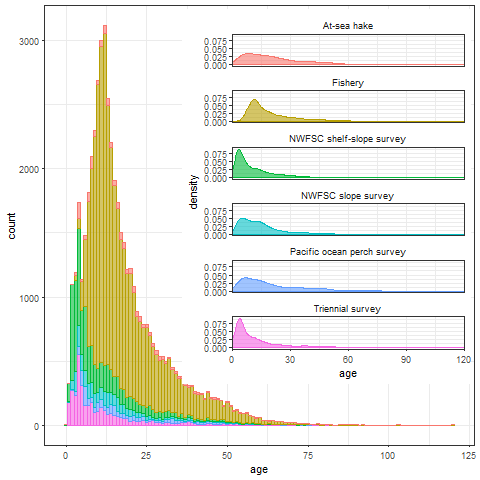
\includegraphics[scale = 0.45]{figures/pop2017_agesbysource.png}
    \end{column}
  \end{columns}
\end{frame}

%-------------------------------------------------------------------------------------
%\section{Data Summary}
%-------------------------------------------------------------------------------------

\subsection{}
\begin{frame}{Data Summary Used in the 2017 Assessment}
  \begin{figure}[ht]
    \begin{center}
      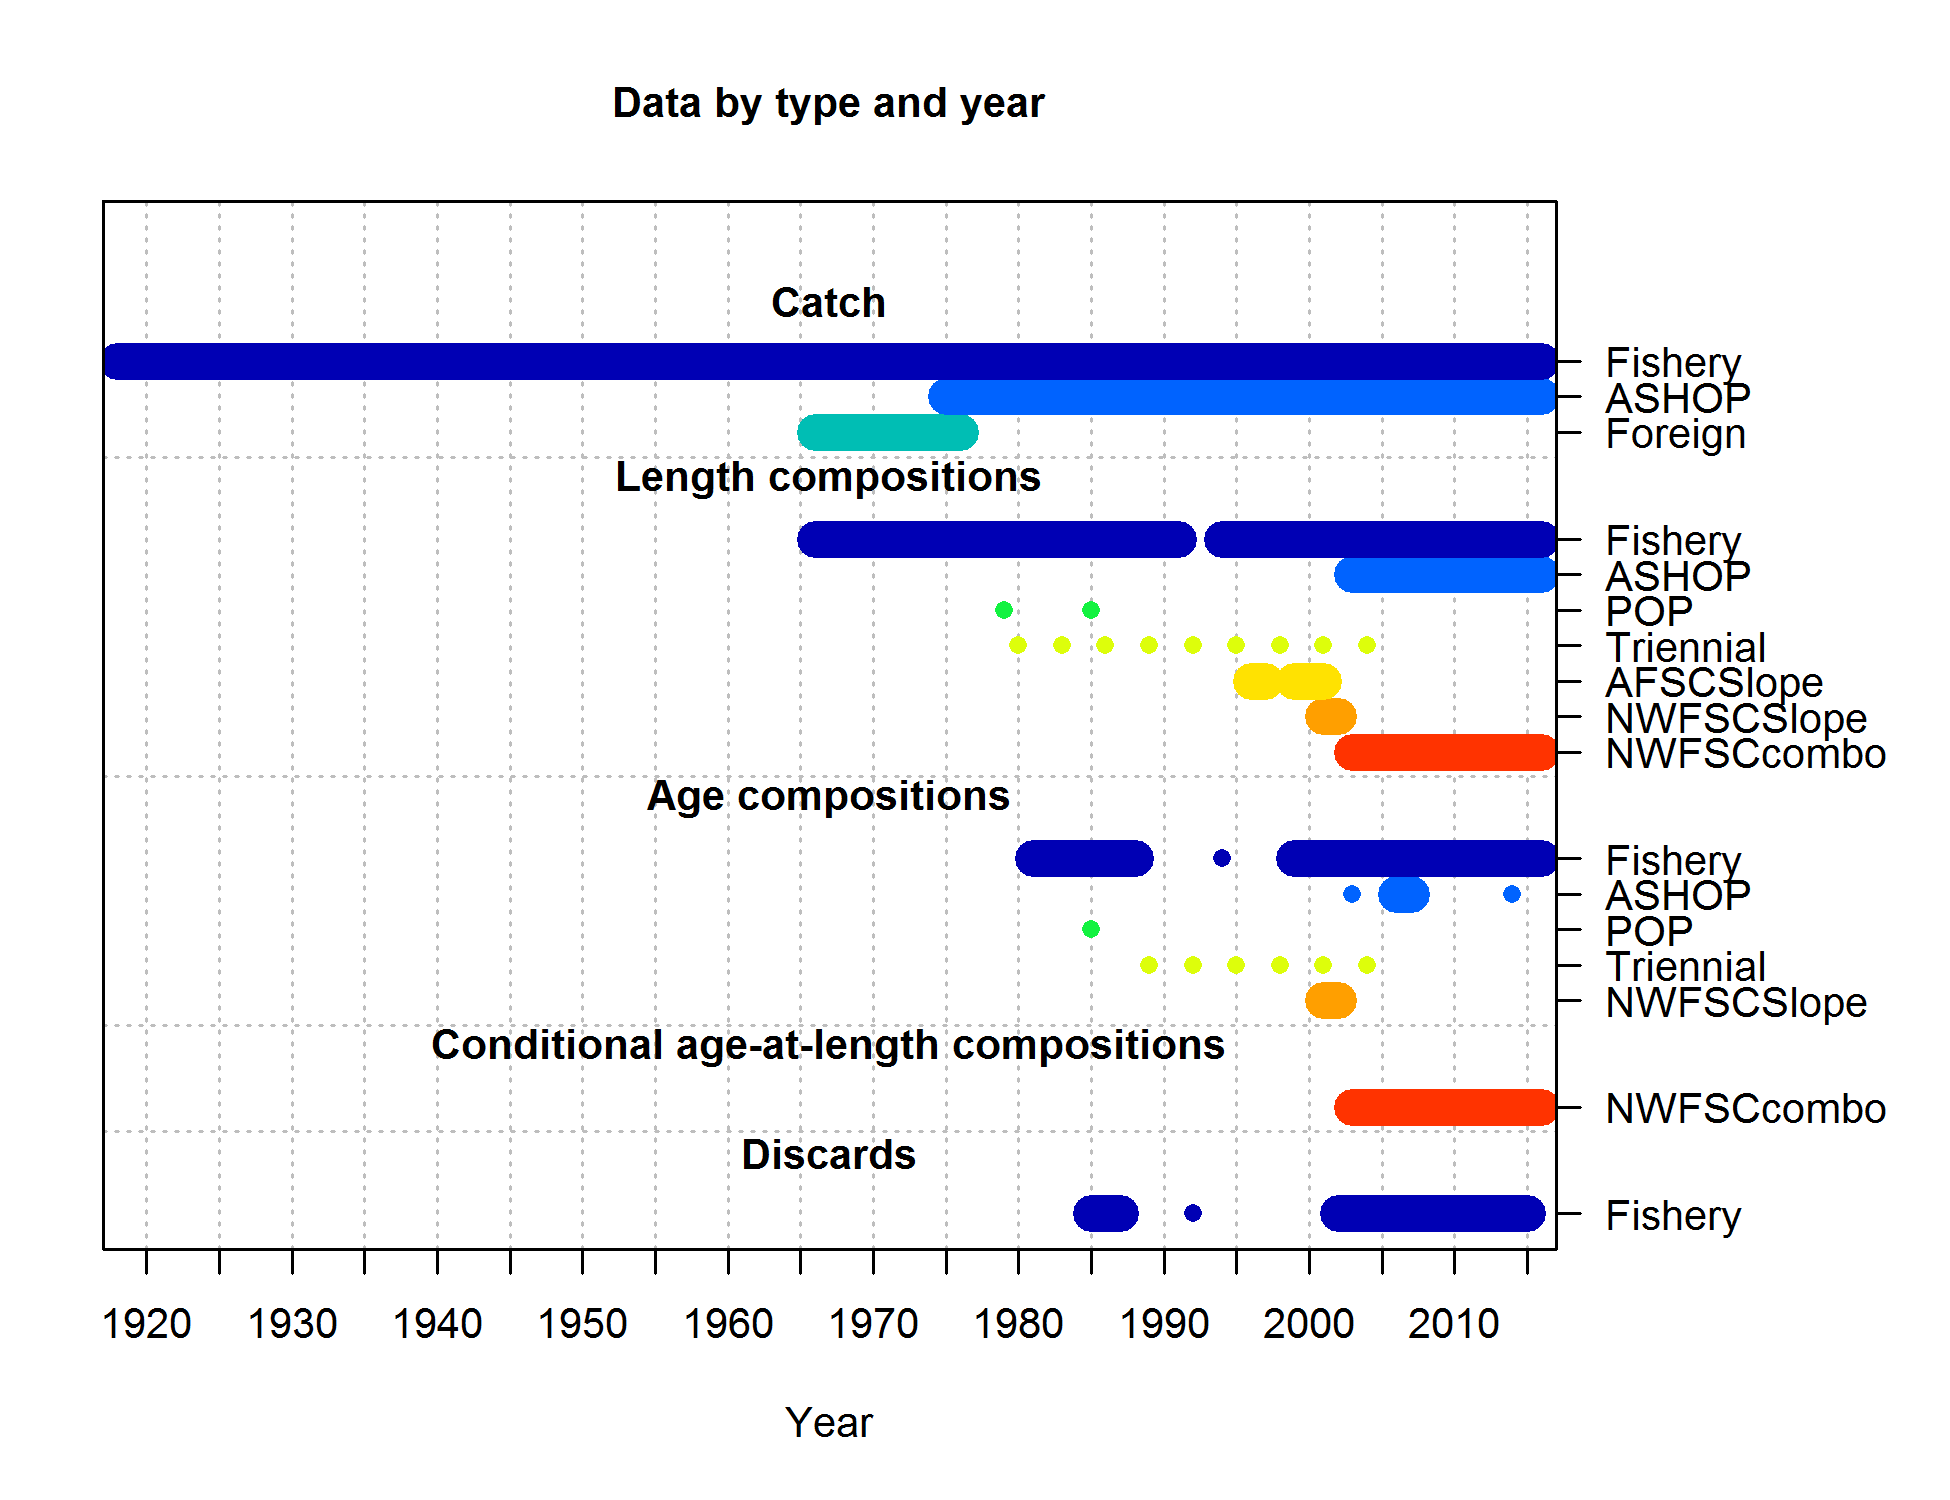
\includegraphics[height=3in]{r4ss/data_plot.png}

    \end{center}
  \end{figure}
\end{frame}


%---------------------------------------------------------------------------------
\section{Removals}
%---------------------------------------------------------------------------------
\subsection{Landing history by state}
\begin{frame}{Landings Data: 2017 vs. 2011}
  \begin{center}
    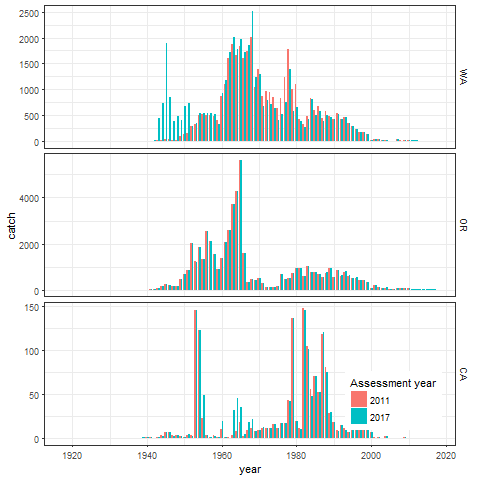
\includegraphics[scale = 0.45]{figures/pop2017_2011vs2017catches_states.png}
  \end{center}
\end{frame}

\begin{frame}{Cummalative catch difference}
  \begin{center}
    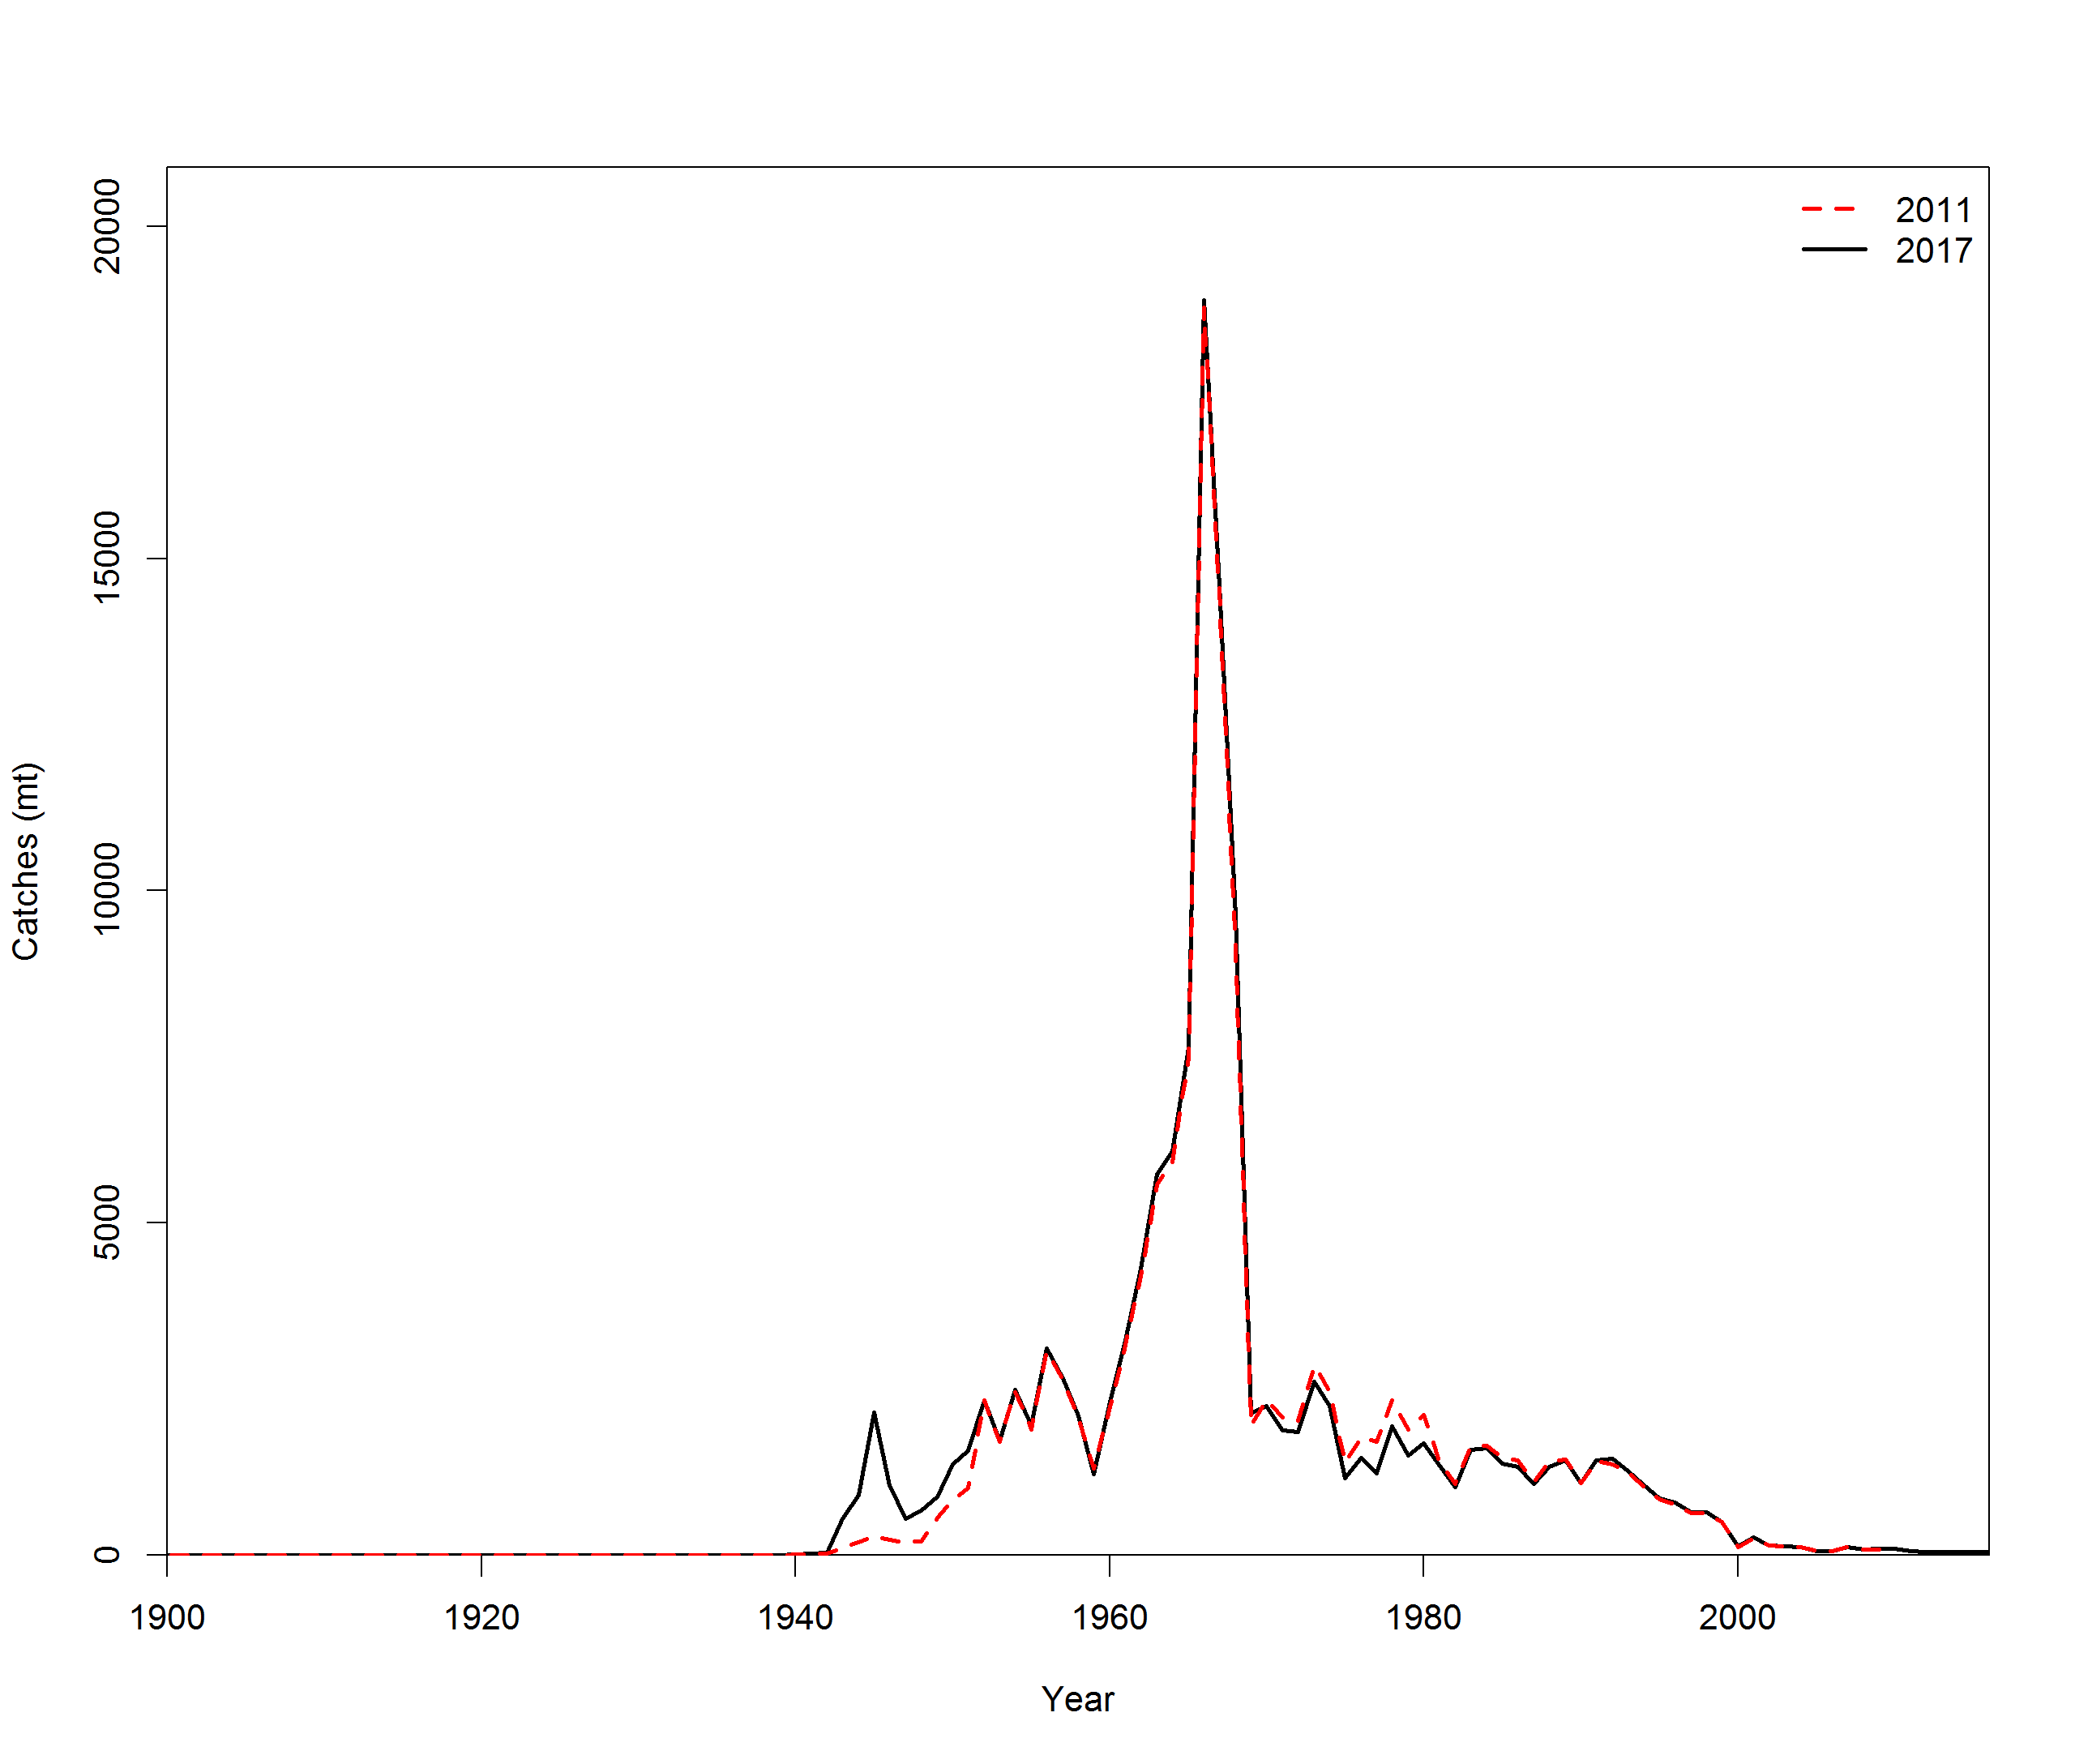
\includegraphics[scale = 0.32, trim={0, 0, 0, 2cm}, clip]{figures/Catch_Comparison.png}
  \end{center}
  *Resulted in $<$ 1\% change in $R0$ 
\end{frame}

\subsection{Discarding practices}
\begin{frame}{Fishery Discard Data}
  \begin{center}
    \includegraphics[scale = 0.40, trim={0, 0, 0, 1cm}, clip]{r4ss/POP_discard_data.png}
  \end{center}

  \begin{tikzpicture}[remember picture, overlay, shift = {(current page.center)}]
    \node[black] at (-2, -2.15) {\small Pikitch};
    \node[black] at (-0.5,-1.5) {\small Management};
    \node[black] at (-0.5, -1.75) {\small Restrictions};
    \node[black] at (2, 1) {\small WCGOP};
    \draw[black, thick, -] (0.5, 0.8) -- (3, 0.8){};
    \node[black] at (2.5, -2) {\small Post-ITQ};
  \end{tikzpicture}
\end{frame}

%---------------------------------------------------------------------------------
\section{Indices of Abundance}
%---------------------------------------------------------------------------------
\subsection{Fishery CPUE}
\begin{frame}{CPUE}
  \begin{center}
      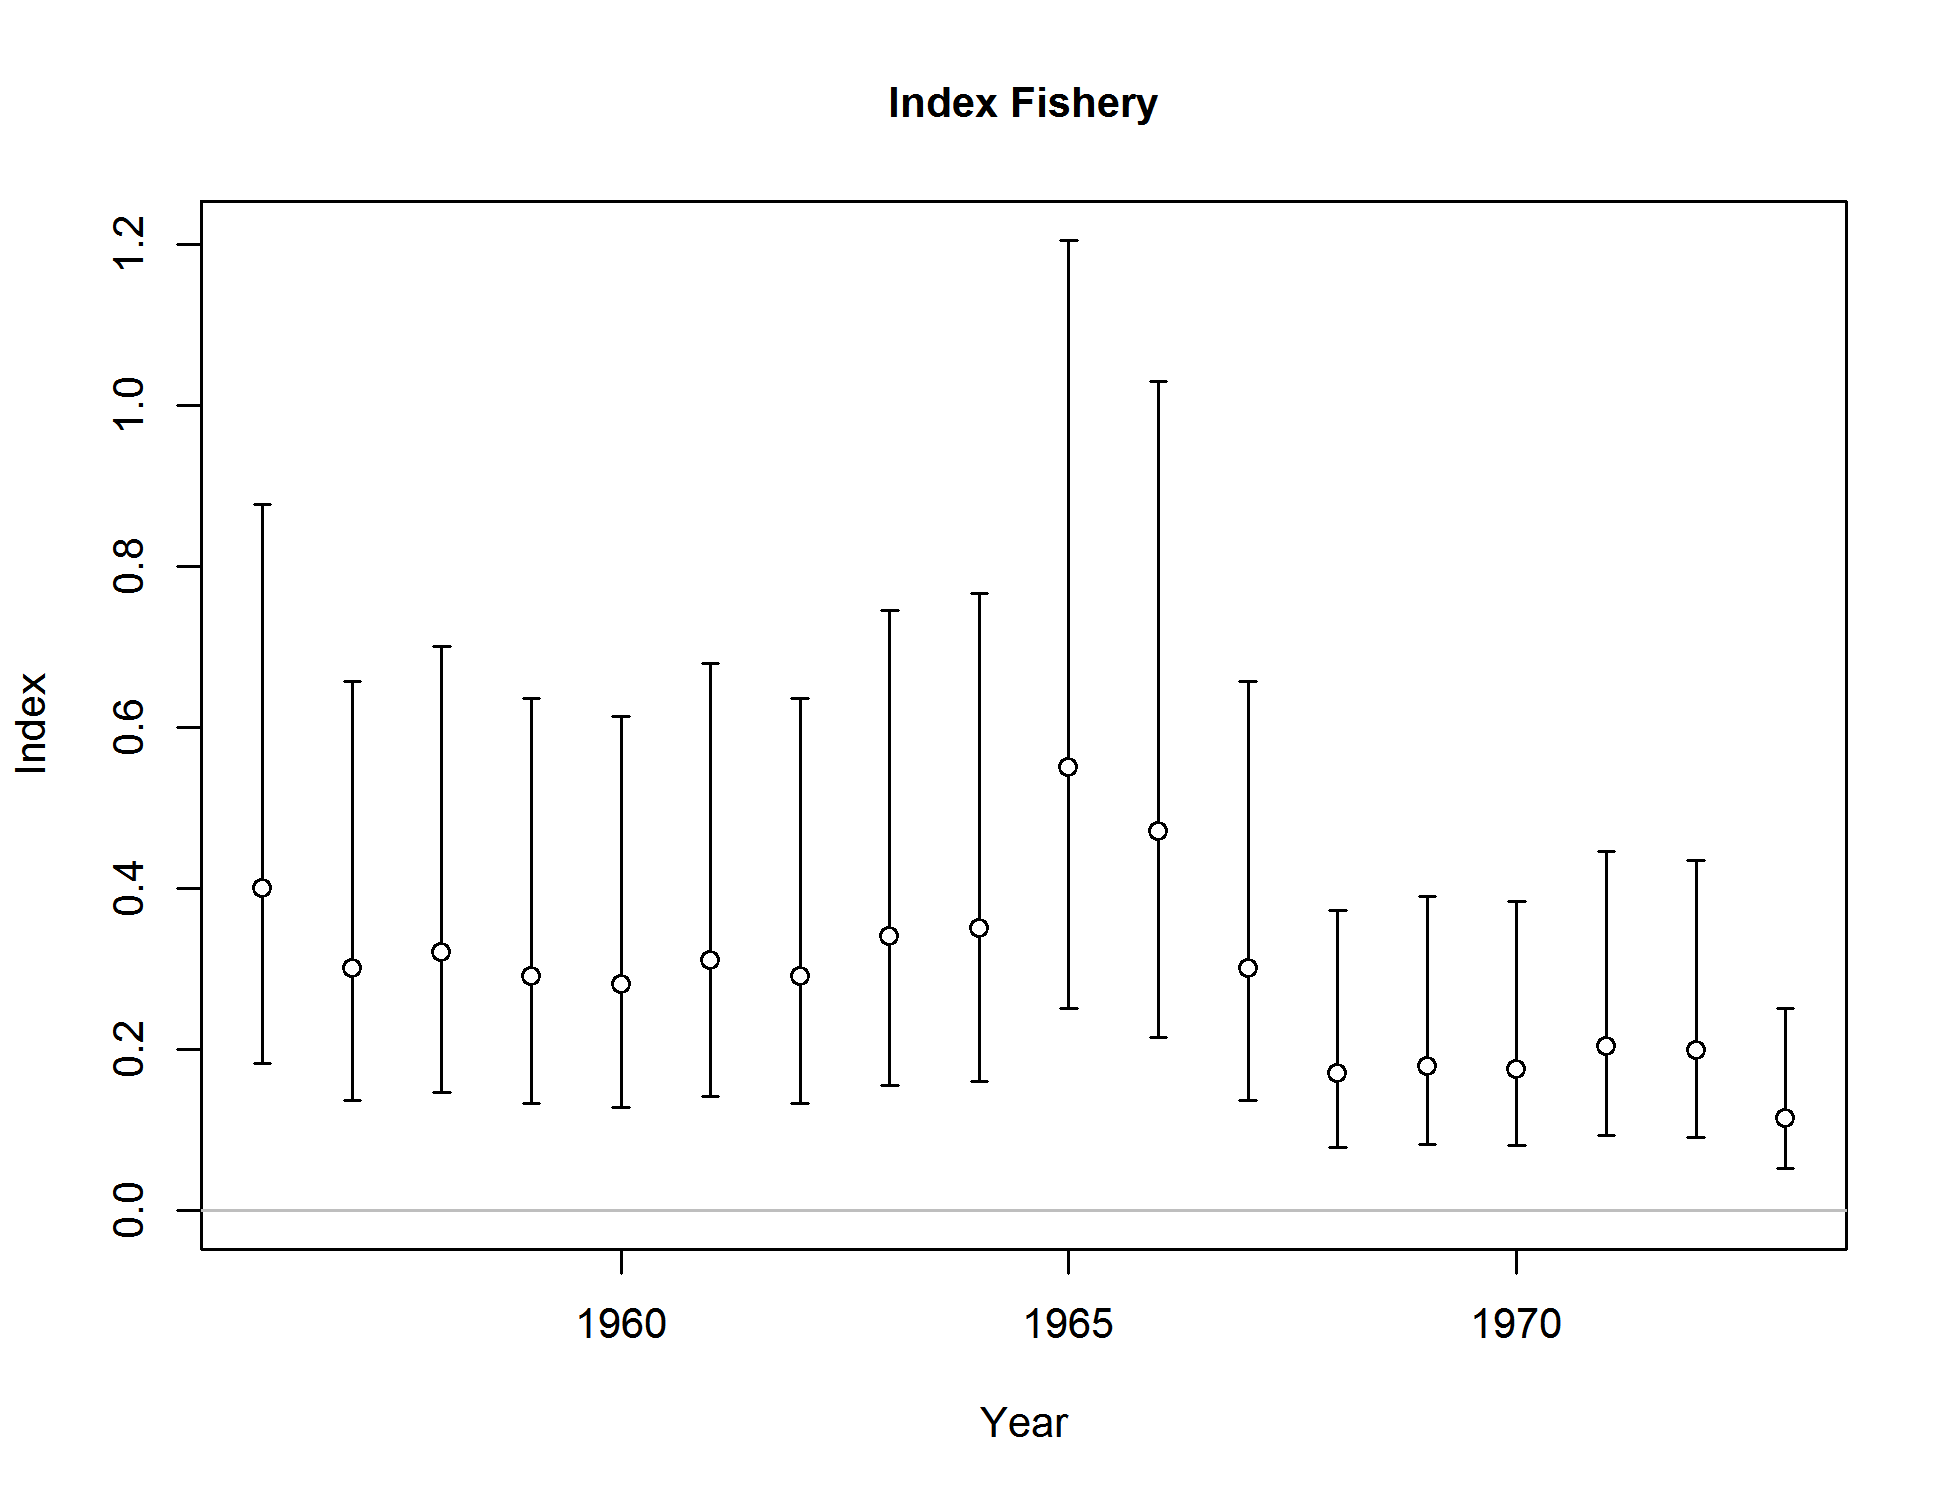
\includegraphics[scale = 0.45]{r4ss/index1_cpuedata_Fishery.png}
  \end{center}
  Gunderson (1977) CPUE from the INPFC Columbia area\\
  *Sensitivity shows little effect on model results when removed.
\end{frame}

\subsection{Survey Indices}
\begin{frame}{Survey Indices}
  \begin{center}
  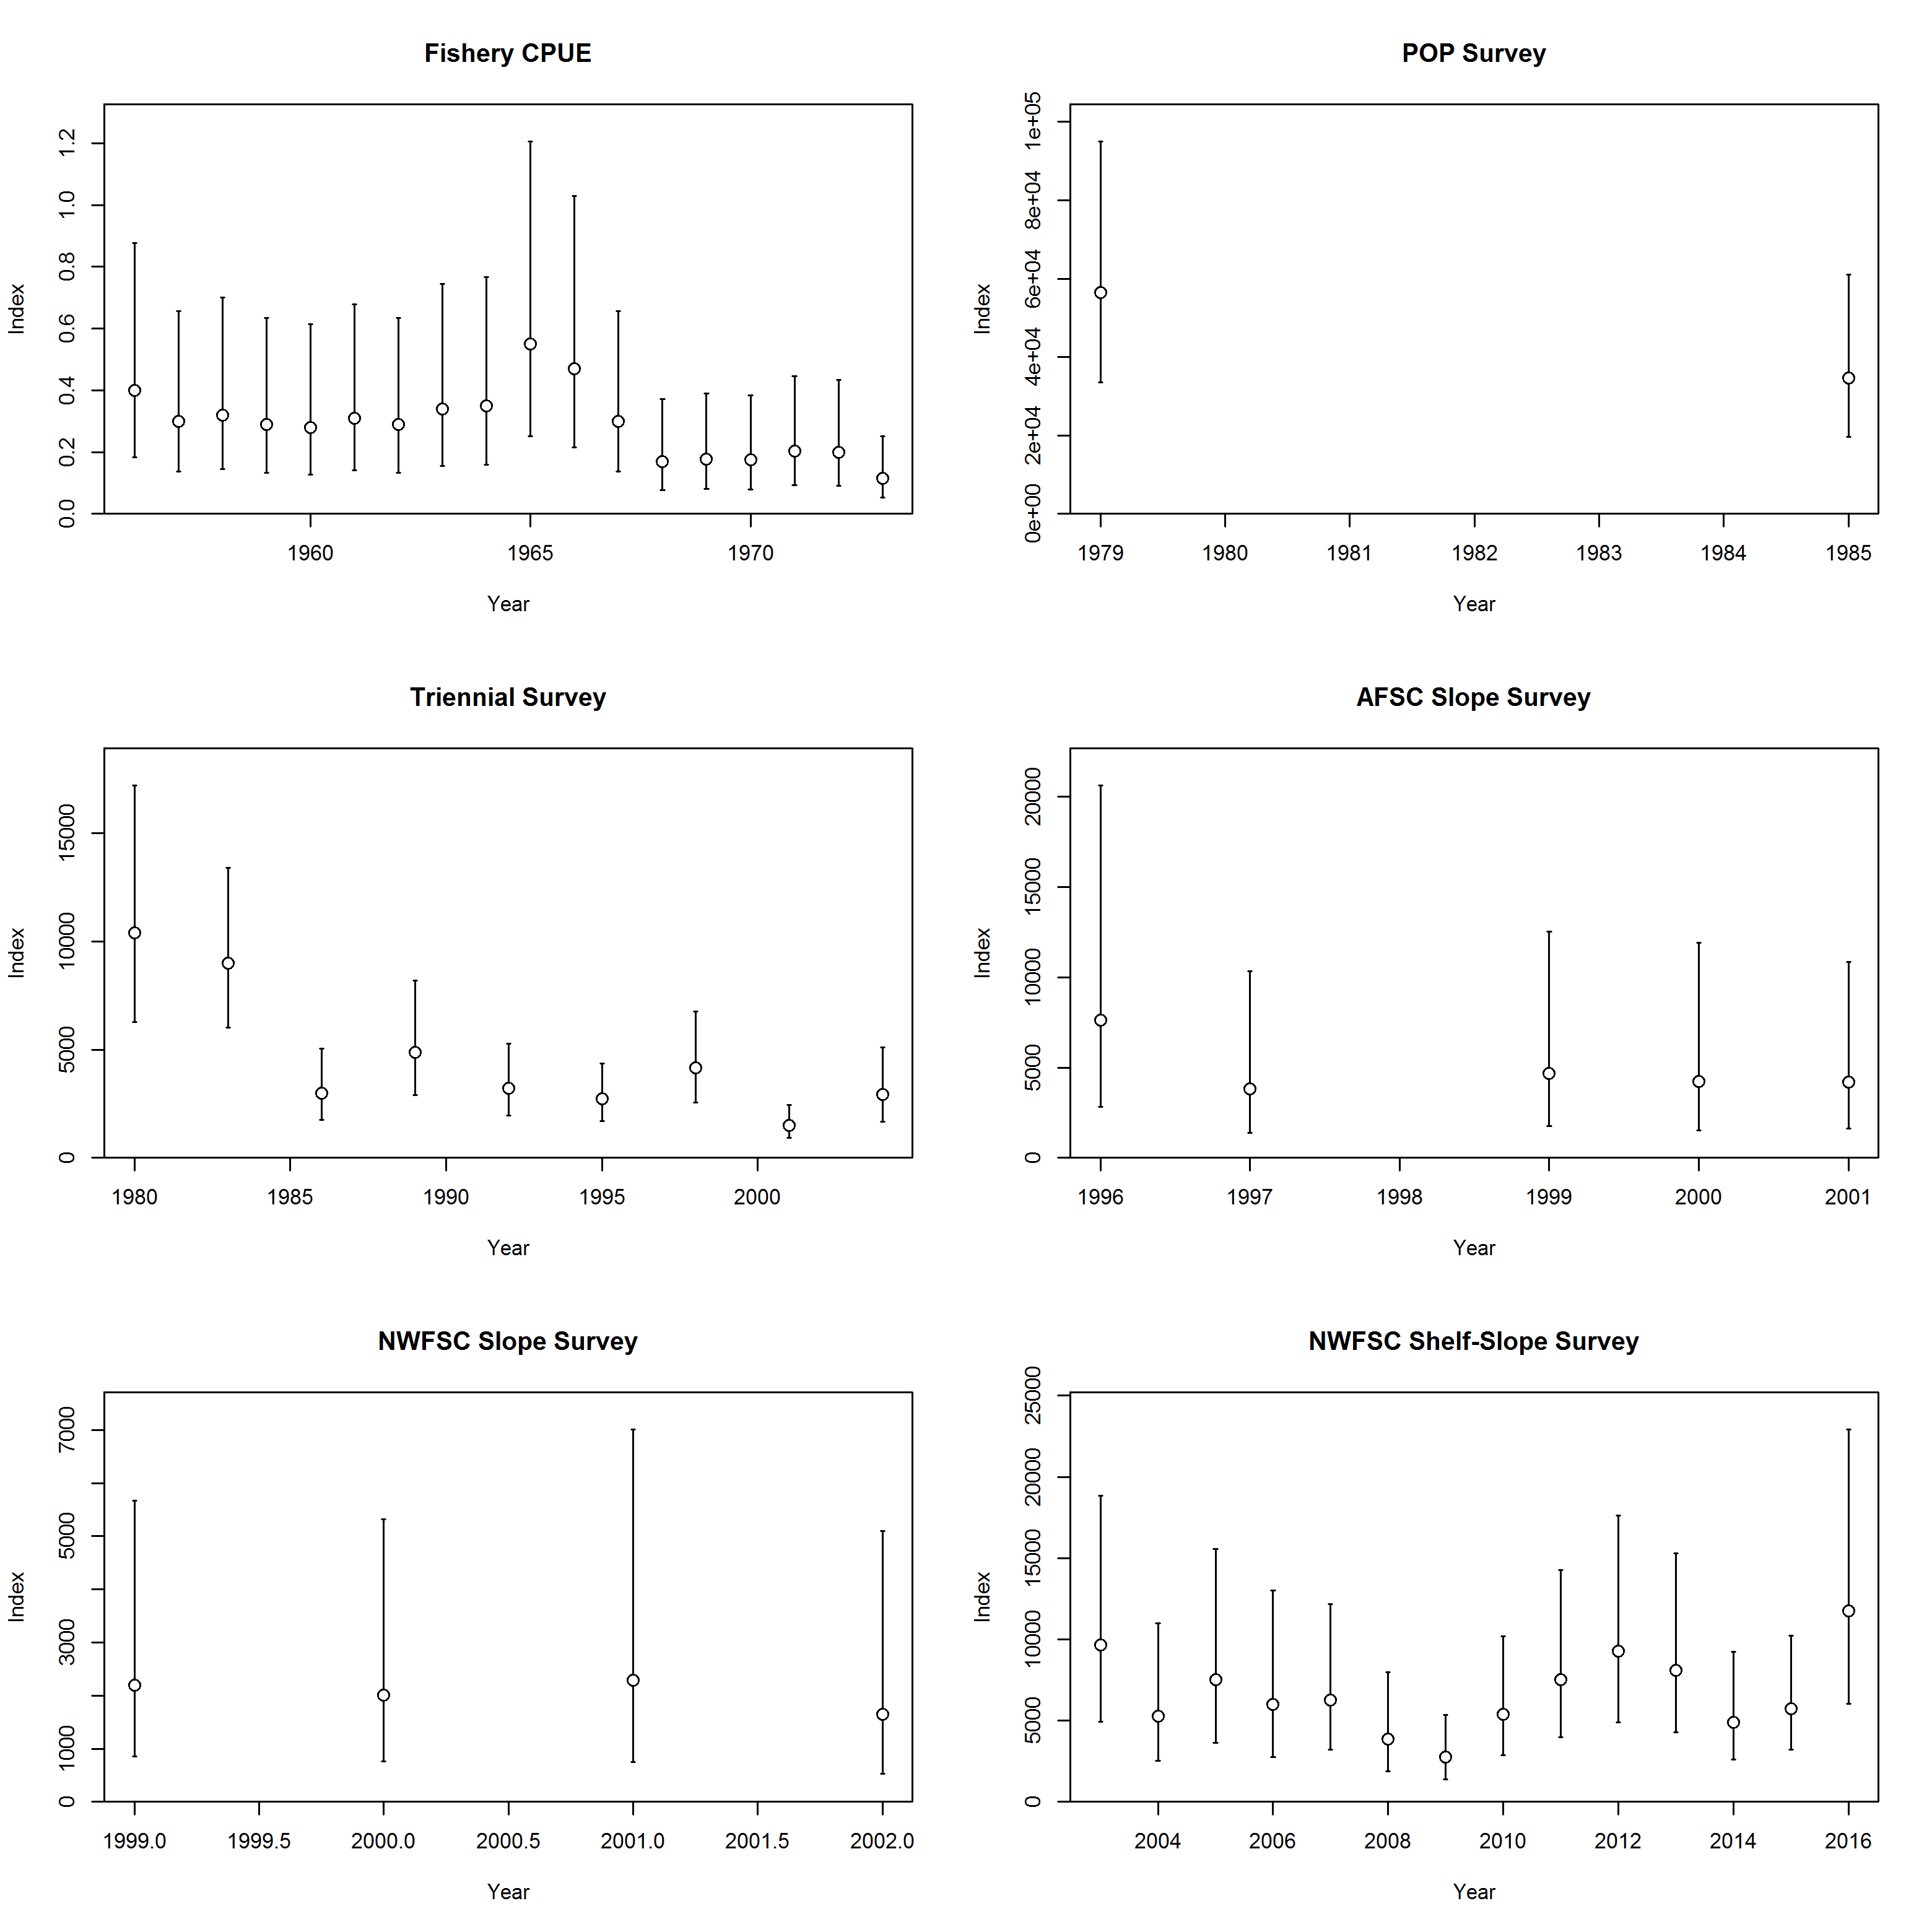
\includegraphics[height = 3in, width = 4in]{figures/Index_Data.png}
  \end{center}
\end{frame}

\begin{frame}{All: standardized}
  \begin{center}
  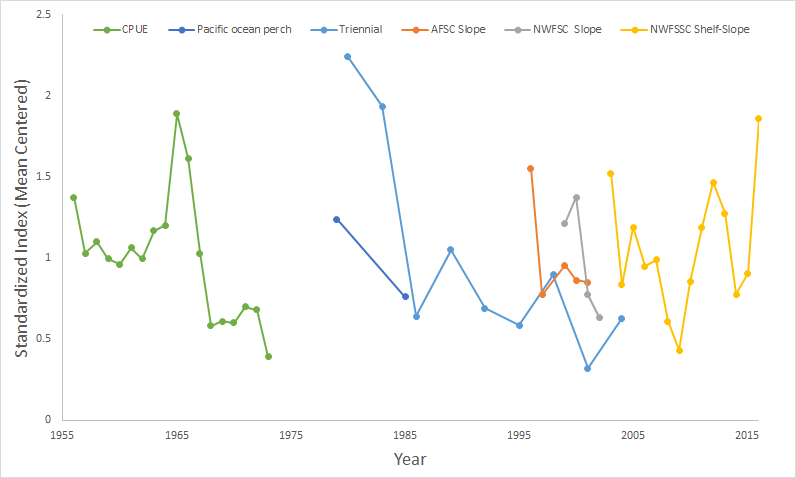
\includegraphics[height = 2.5in, width = 4in]{figures/standardized_index.png}
  \end{center}
\end{frame}

%\begin{frame}{Survey Indices: 2011 vs. 2017}
%\end{frame}

%---------------------------------------------------------------------------------
\section{Length Compositions}
%---------------------------------------------------------------------------------
\subsection{Fishery Lengths}
\begin{frame}{Fishery Length Data}
  Fishery length data used in the 2017 assessment:
  \begin{itemize}
    \item Fishery: bottom trawl, mid-water trawl, fixed gear
      \begin{itemize}
        \item Retained Lengths 1966-2016
        \item Discarded Lengths 1986 (Pikitch), 2004-2015
      \end{itemize}
    \item At-sea hake fishery
      \begin{itemize}
        \item All (Retained and Discarded) Lengths 2003-2016
      \end{itemize}
  \end{itemize}
\end{frame}

\begin{frame}{Fishery Lengths: Retained}
  \begin{center}
    \includegraphics[scale = 0.50]{r4ss/comp_lendat_bubflt1mkt2_page4.png}
  \end{center}
  \onslide<2->
  \begin{tikzpicture}[remember picture, overlay, shift = {(current page.center)}]
    \draw[black, thick, -] (3,   -0.6) -- (3.4, -0.1);
    \draw[black, thick, -] (-2,   -0.6) -- (-1.6, -0.1);
  \end{tikzpicture}
\end{frame}

\begin{frame}{Fishery Lengths: Discarded}
  \begin{center}
    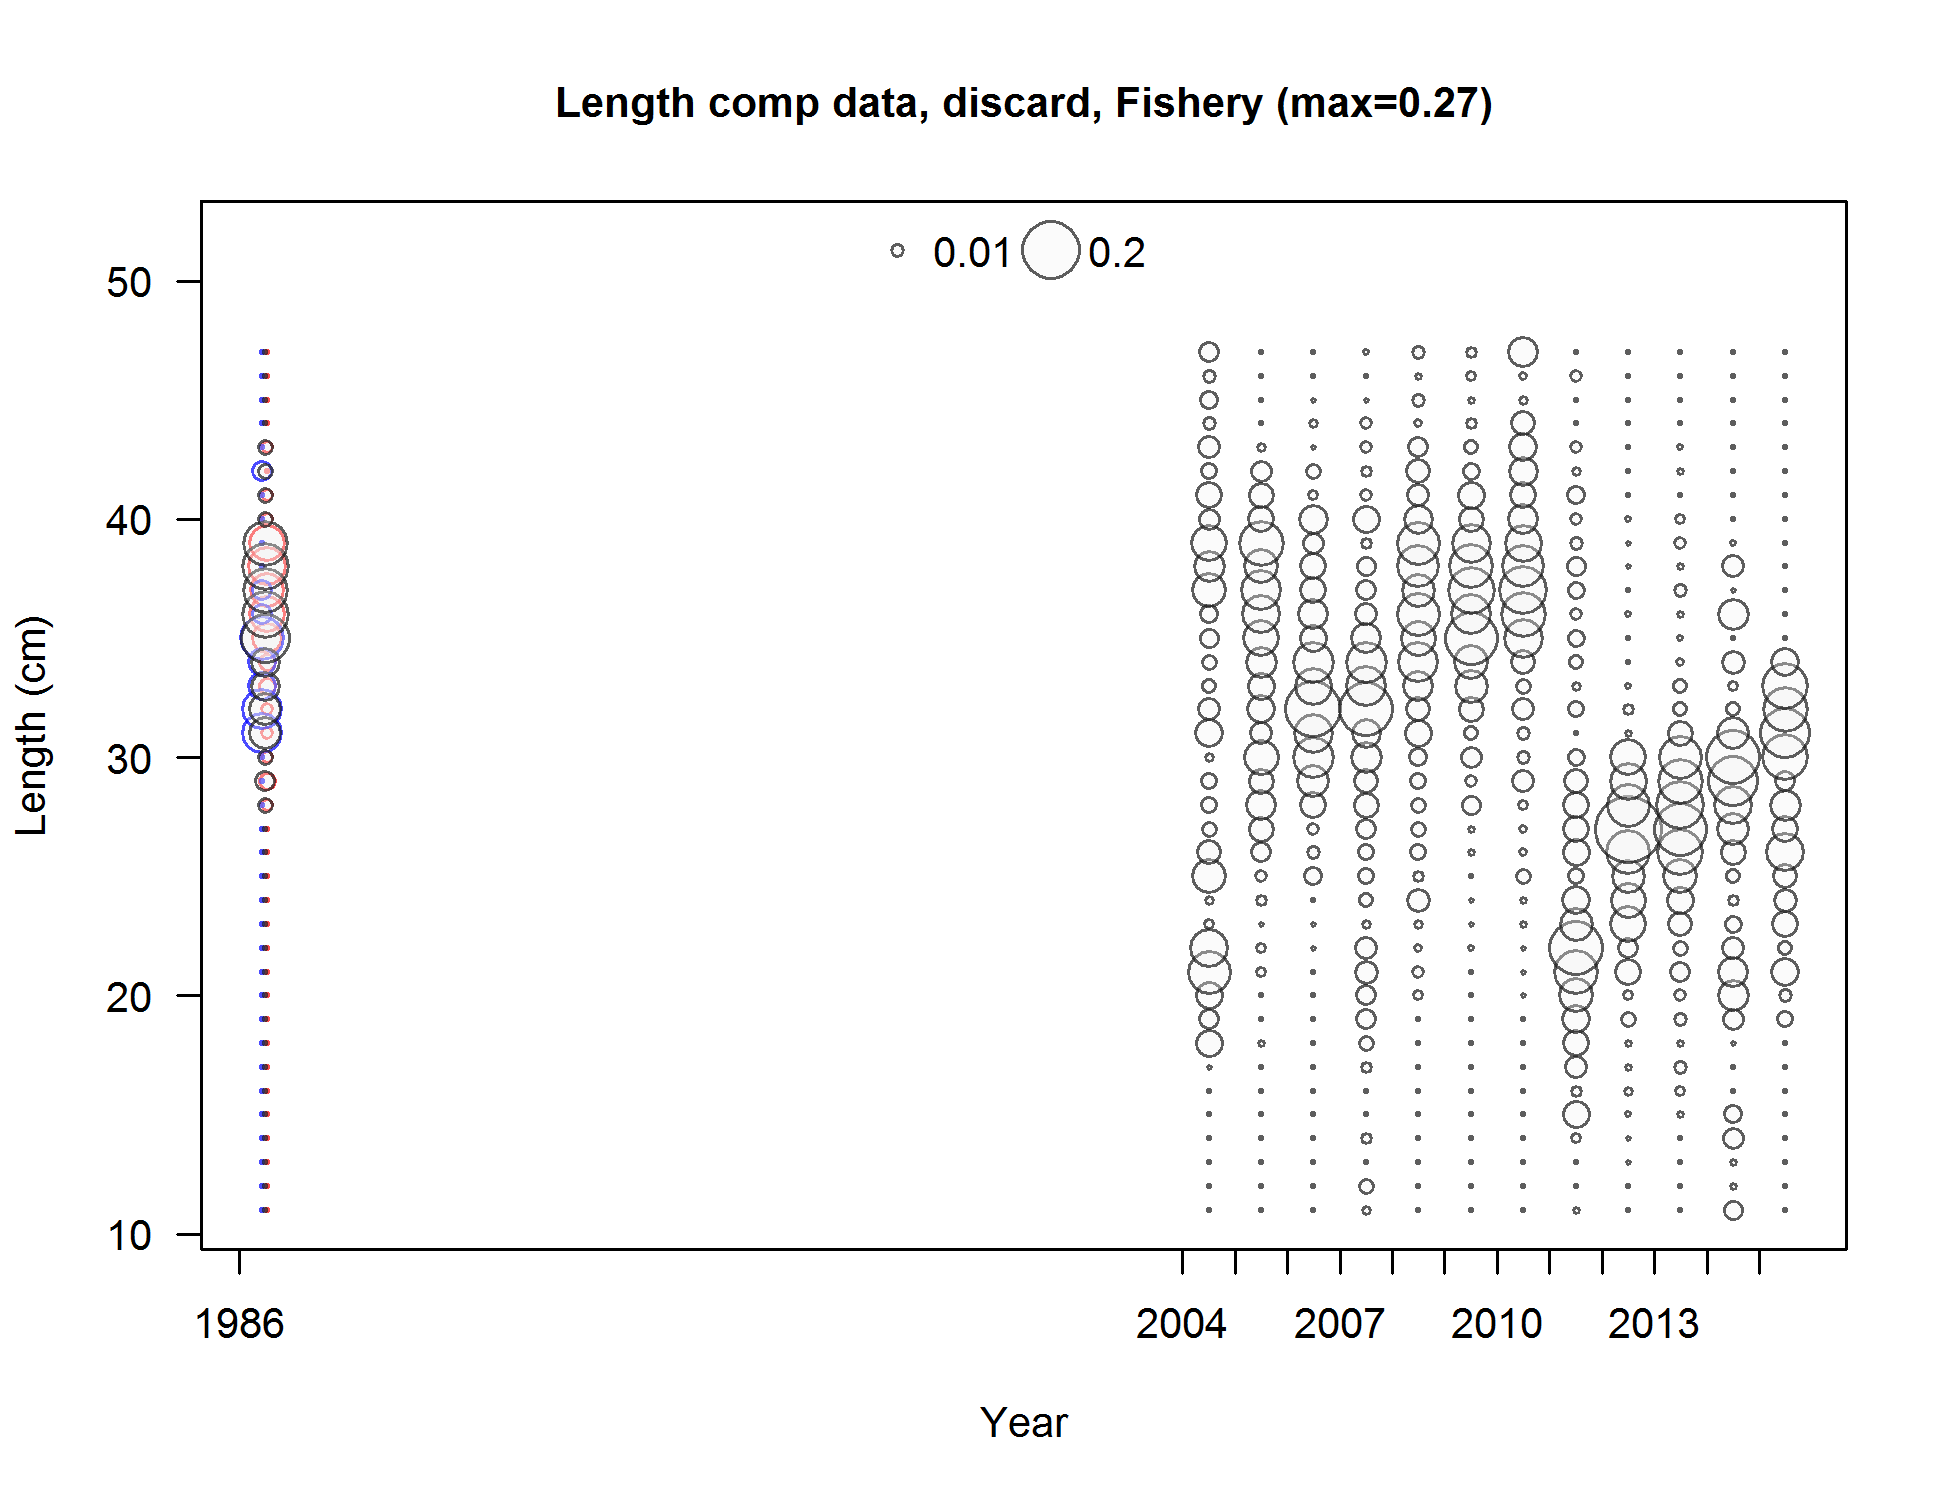
\includegraphics[scale = 0.50]{r4ss/comp_lendat_bubflt1mkt1.png}
  \end{center}
\end{frame}

\begin{frame}{At-sea hake lengths}
  \begin{center}
    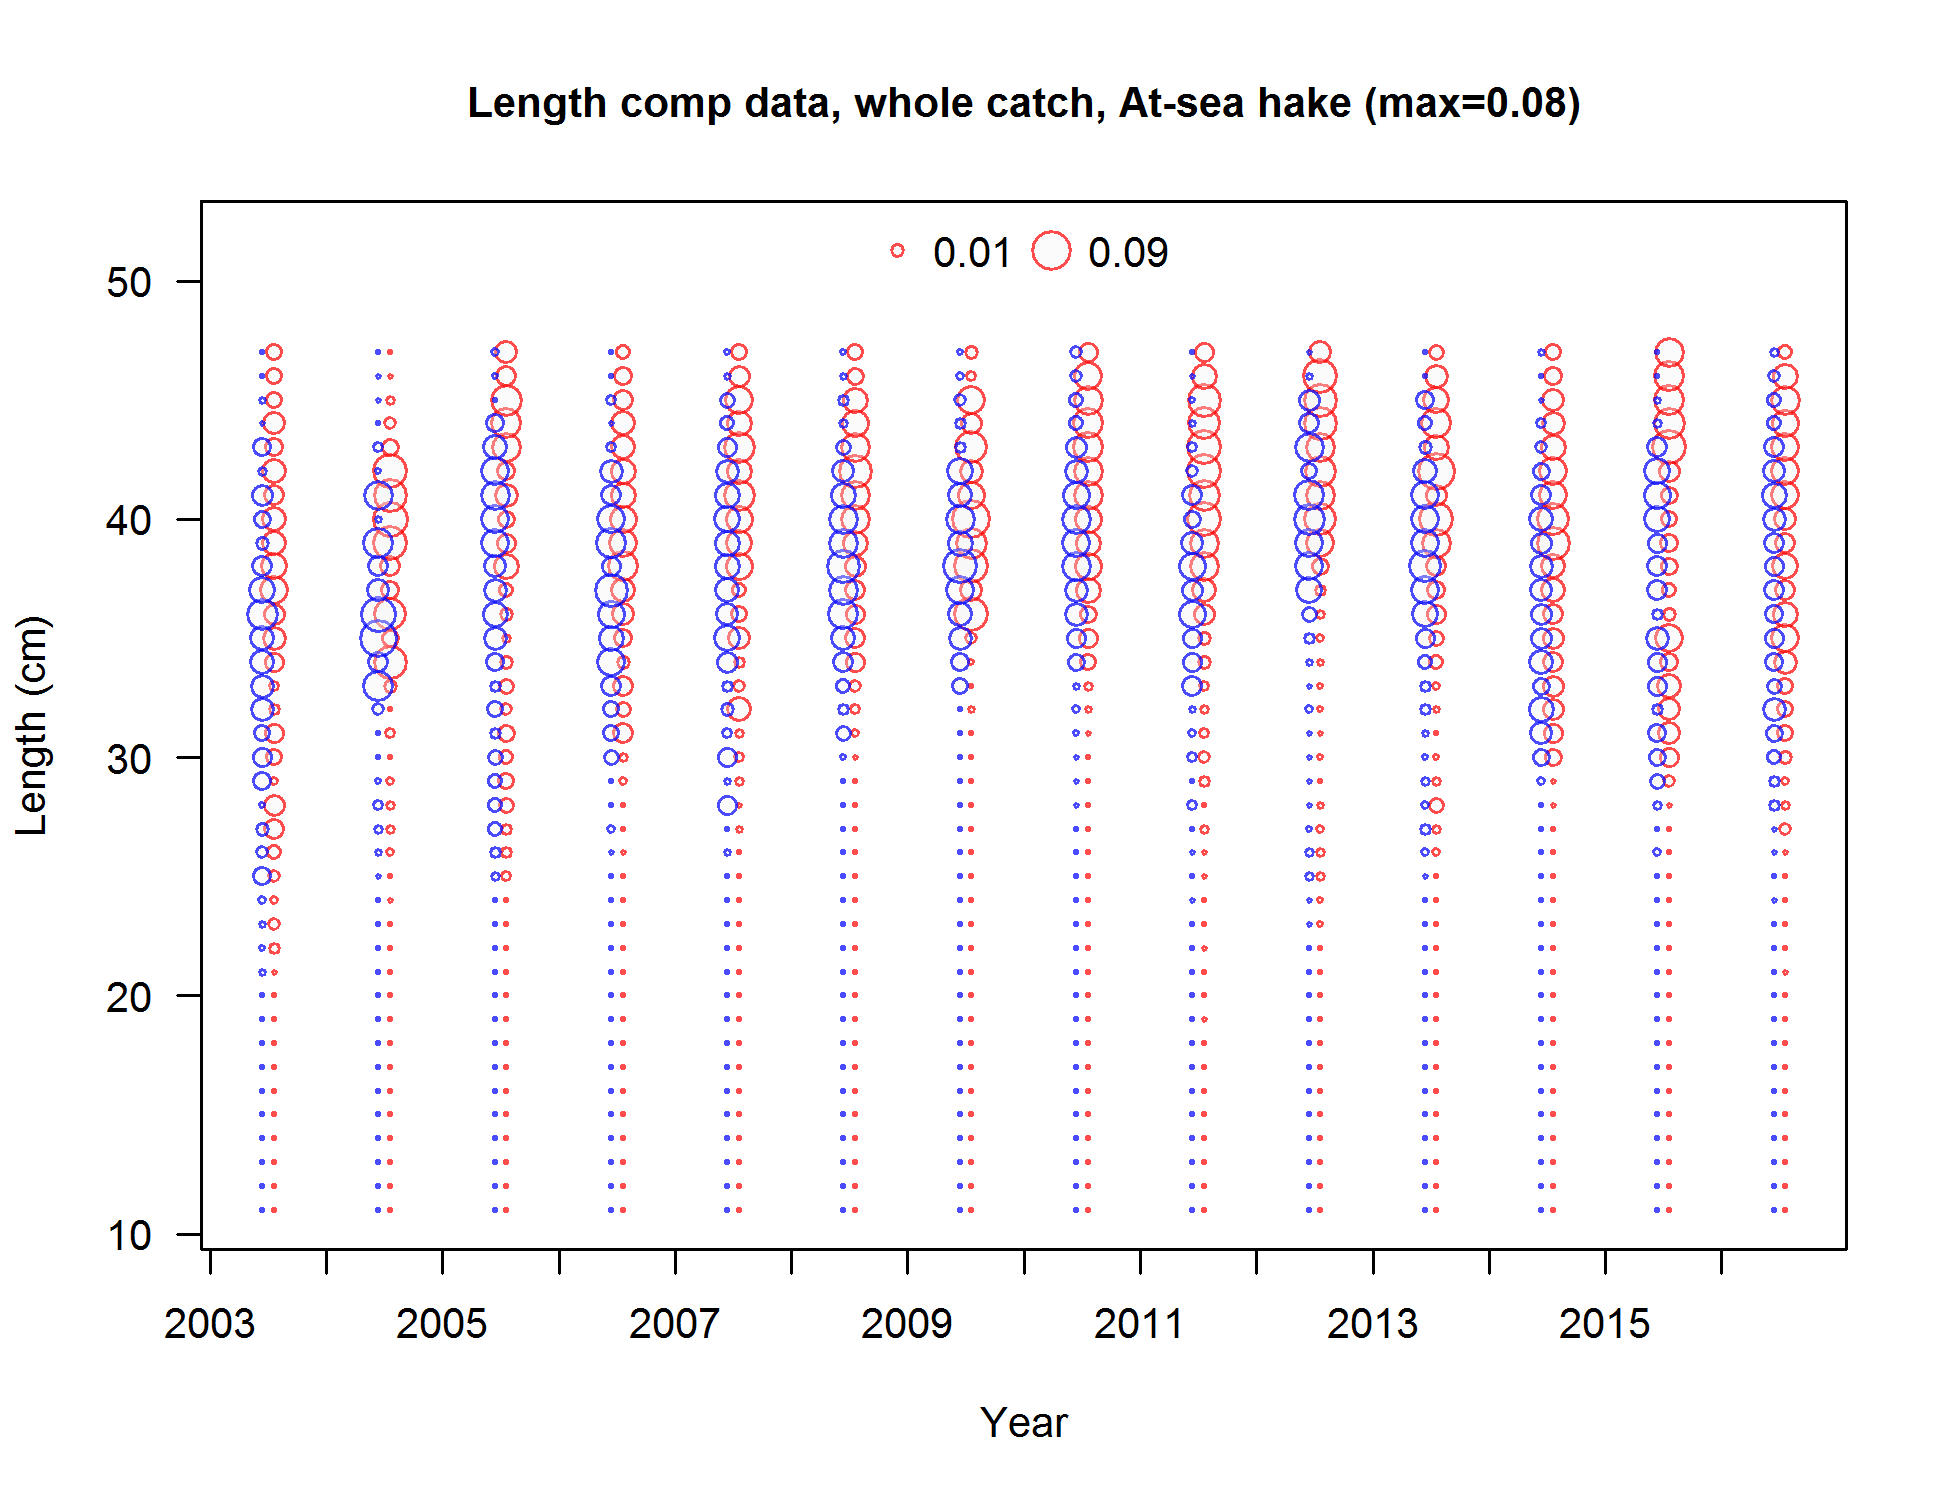
\includegraphics[scale = 0.50]{r4ss/comp_lendat_bubflt2mkt0.png}
  \end{center}
\end{frame}

\subsection{Survey Lengths}
\begin{frame}{Survey Length Data}
  Survey length data used in the 2017 assessment:
  \begin{itemize}
    \item Pacific ocean perch survey
      \begin{itemize}
        \item 1979 and 1985
      \end{itemize}
    \item Triennial survey
      \begin{itemize}
        \item 1980, 1983, 1896, 1989, 1992, 1995, 1998, 2001, 2004
      \end{itemize}
    \item AFSC slope survey
      \begin{itemize}
        \item 1996, 1997, 1999-2001
      \end{itemize}
    \item NWFSC slope survey
      \begin{itemize}
        \item 2001 and 2002
      \end{itemize}
    \item NWFSC shelf-slope survey
      \begin{itemize}
        \item 2003-2016
      \end{itemize}
  \end{itemize}
\end{frame}

\begin{frame}{Pacific ocean perch survey lengths}
  \begin{center}
    \includegraphics[scale = 0.50]{r4ss/comp_lendat_bubflt4mkt0.png}
  \end{center}
\end{frame}

\begin{frame}{Triennial survey lengths}
  \begin{center}
    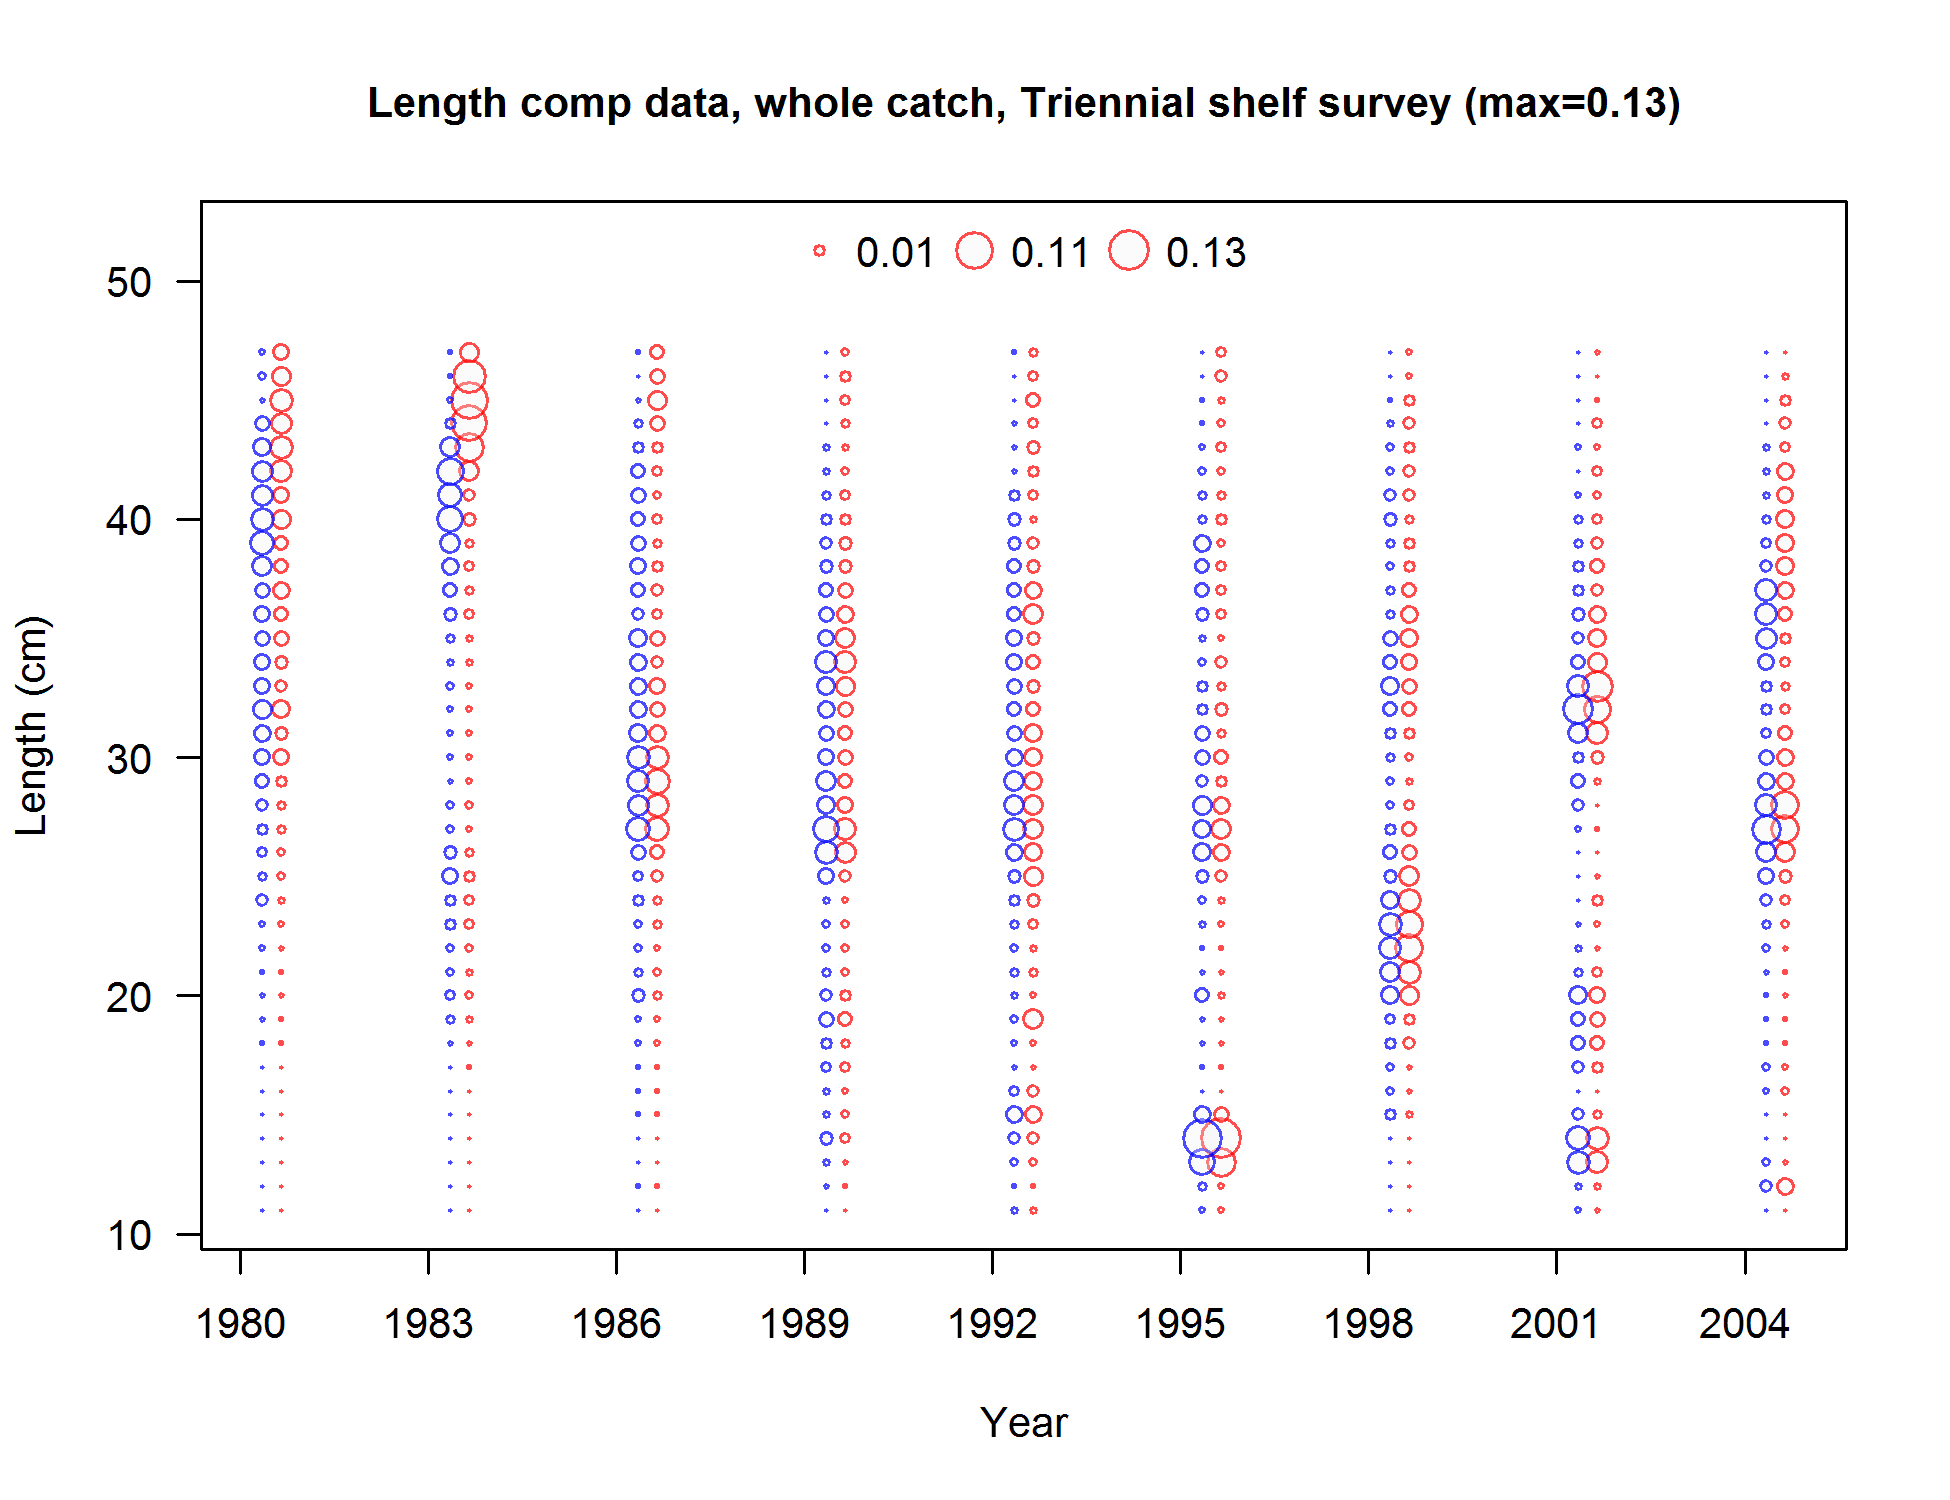
\includegraphics[scale = 0.50]{r4ss/comp_lendat_bubflt5mkt0.png}
  \end{center}
\end{frame}

\begin{frame}{AFSC slope survey lengths}
  \begin{center}
    \includegraphics[scale = 0.50]{r4ss/comp_lendat_bubflt6mkt0.png}
  \end{center}
\end{frame}

\begin{frame}{NWFSC slope survey lengths}
  \begin{center}
    \includegraphics[scale = 0.50]{r4ss/comp_lendat_bubflt7mkt0.png}
  \end{center}
\end{frame}

\begin{frame}{NWFSC shelf-slope survey lengths}
  \begin{center}
    \includegraphics[scale = 0.50]{r4ss/comp_lendat_bubflt8mkt0.png}
  \end{center}
\end{frame}

\begin{frame}{Aggregated lengths by source}
  \begin{center}
    \includegraphics[scale = 0.50]{r4ss/comp_lendat__aggregated_across_time.png}
  \end{center}
\end{frame}

%---------------------------------------------------------------------------------
\section{Age Compositions}
%---------------------------------------------------------------------------------
\subsection{Fishery Ages}
\begin{frame}{Fishery Age Data}
  Fishery age data used in the 2017 assessment:
  \begin{itemize}
    \item Fishery: bottom trawl, mid-water trawl, fixed gear
      \begin{itemize}
        \item 1981-1988, 1994, 1999-2016
      \end{itemize}
    \item At-sea hake fishery
      \begin{itemize}
        \item 2003, 2006, 2007, 2014
      \end{itemize}
  \end{itemize}
\end{frame}

\begin{frame}{Fishery Ages}
  \begin{center}
    \includegraphics[scale = 0.50]{r4ss/comp_agedat_bubflt1mkt2_page2.png}
  \end{center}
\end{frame}

\begin{frame}{At-sea hake Ages}
  \begin{center}
    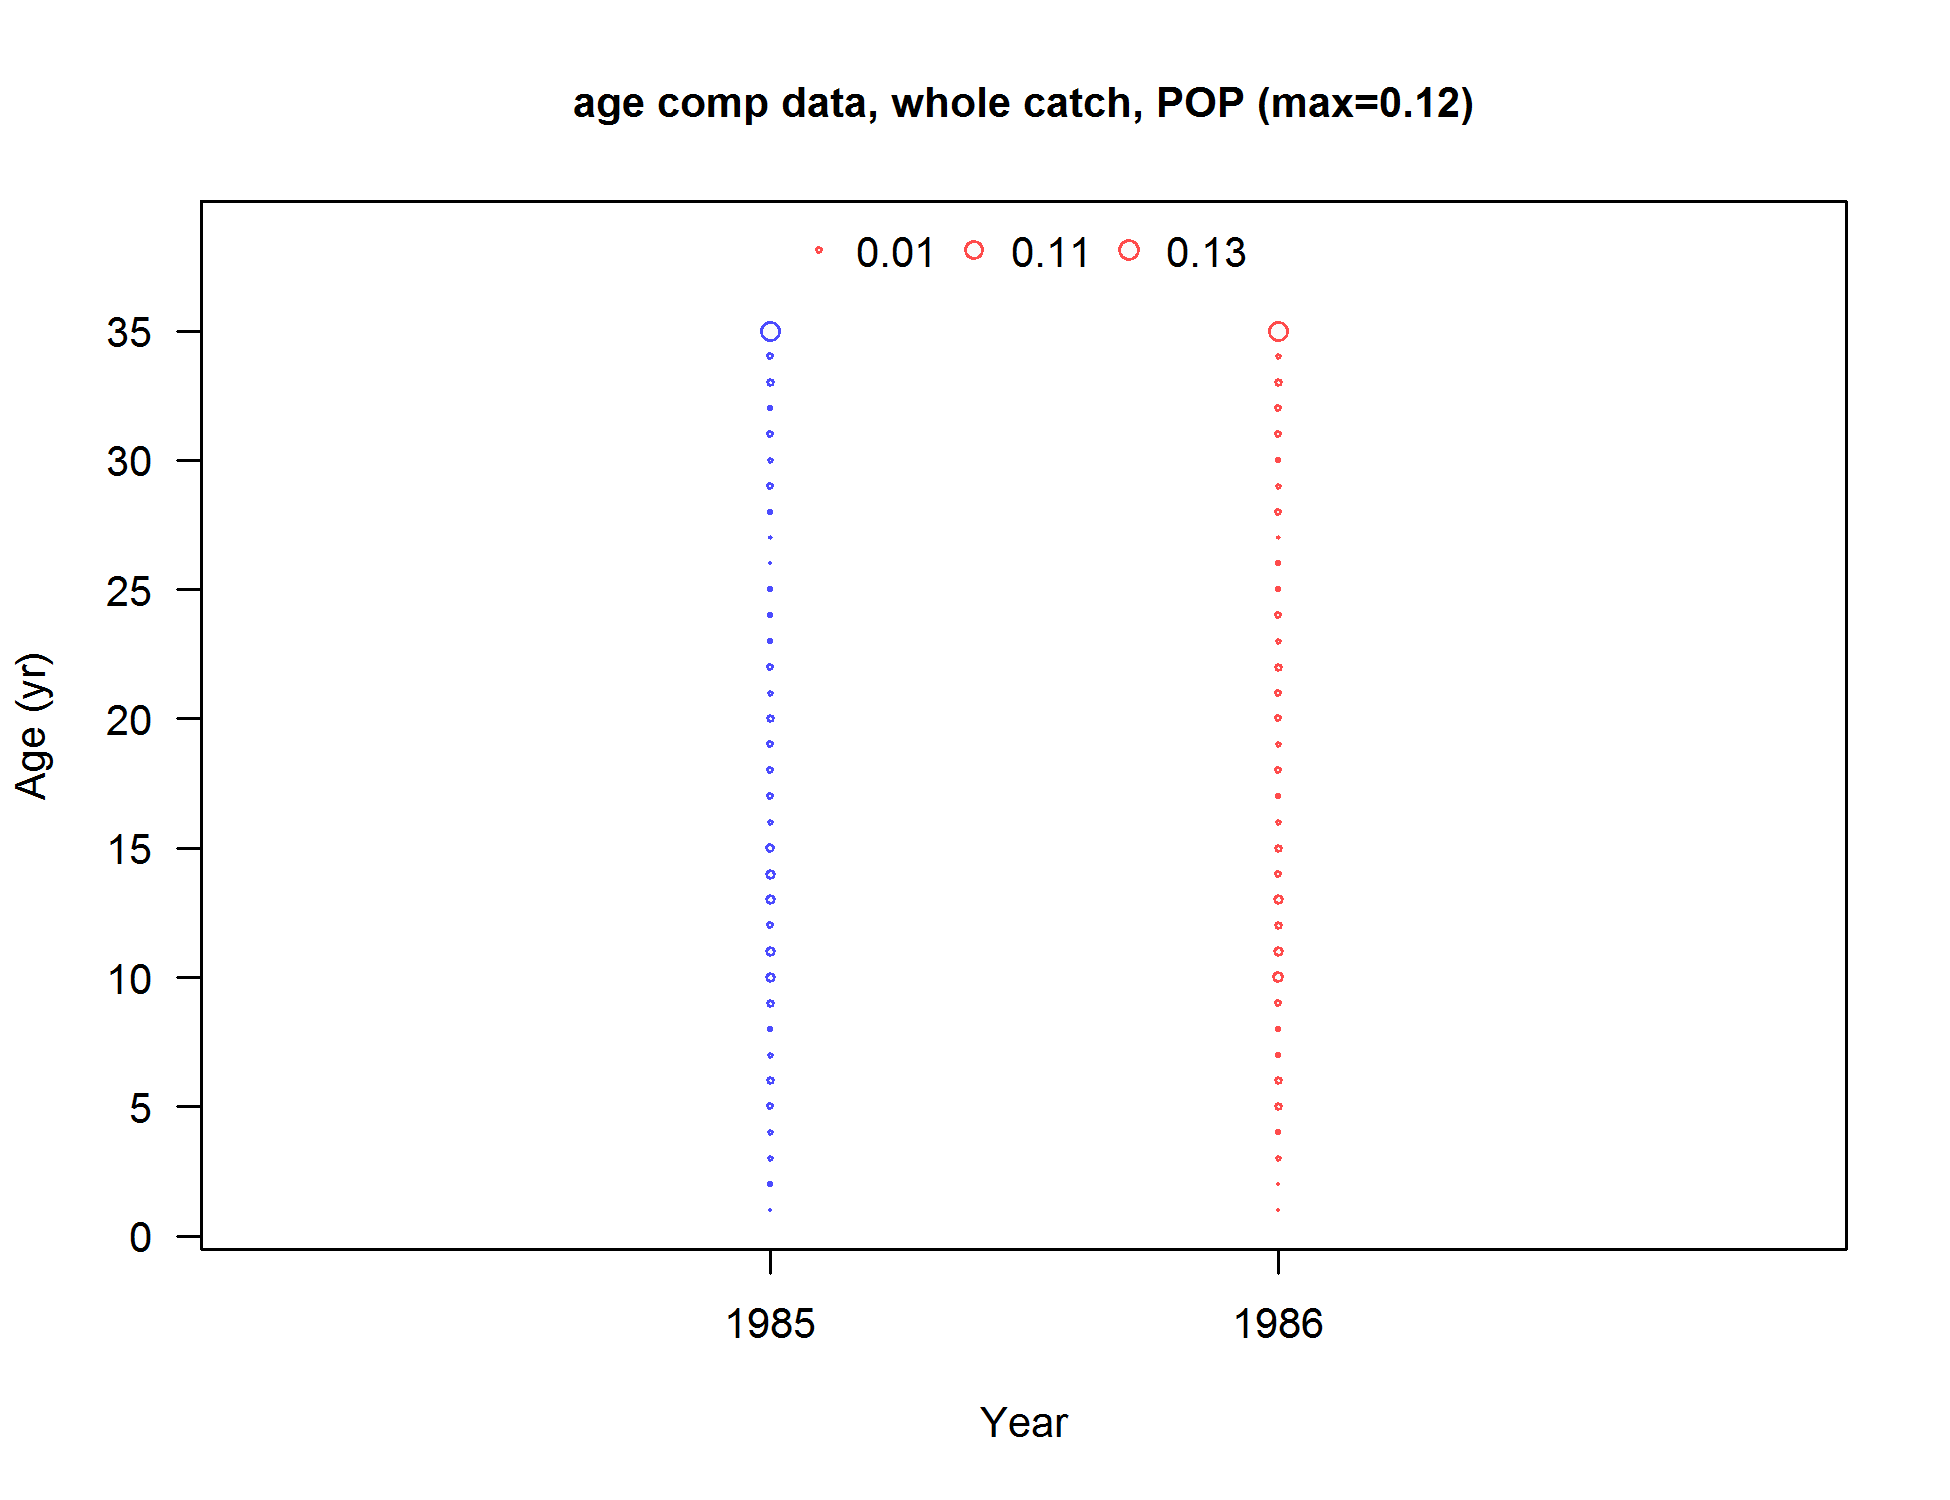
\includegraphics[scale = 0.50]{r4ss/comp_agedat_bubflt2mkt0.png}
  \end{center}
\end{frame}

\subsection{Survey Ages}
\begin{frame}{Survey Age Data}
  Survey age data used in the 2017 assessment:
  \begin{itemize}
    \item Pacific ocean perch survey
      \begin{itemize}
        \item 1985
      \end{itemize}
    \item Triennial survey
      \begin{itemize}
        \item 1989, 1992, 1995, 1998, 2001, 2004
      \end{itemize}
    \item NWFSC slope survey
      \begin{itemize}
        \item 2001 and 2002
      \end{itemize}
    \item NWFSC shelf-slope survey
      \begin{itemize}
        \item 2003-2016
      \end{itemize}
  \end{itemize}
\end{frame}

\begin{frame}{Pacific ocean perch ages}
  \begin{center}
    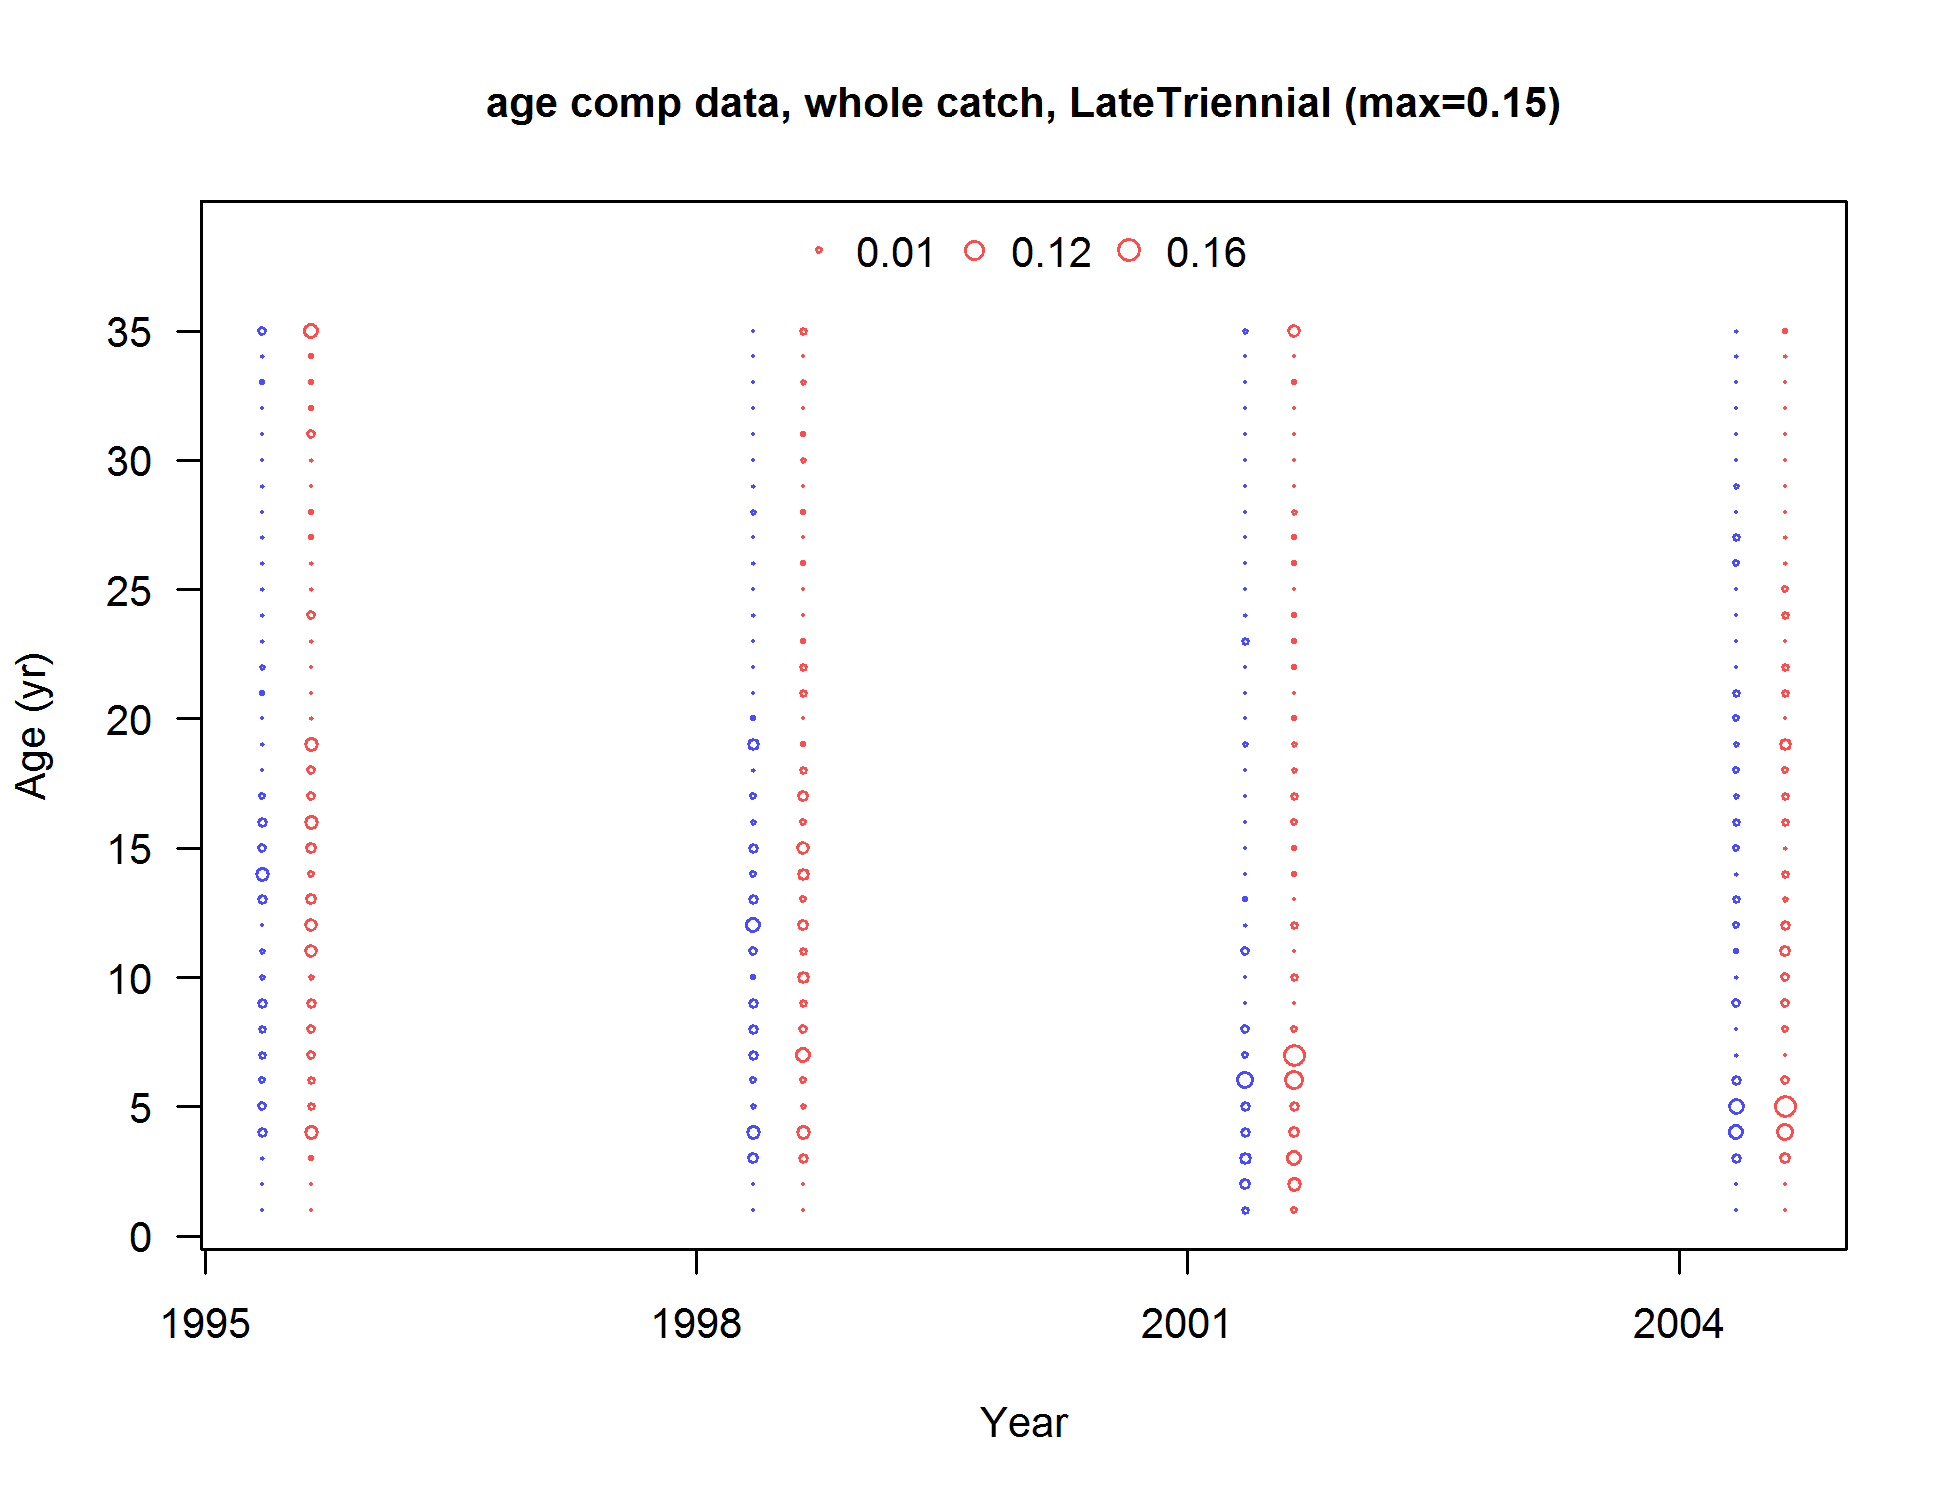
\includegraphics[scale = 0.50]{r4ss/comp_agedat_bubflt4mkt0.png}
  \end{center}
\end{frame}

\begin{frame}{Triennial survey ages}
  \begin{center}
    \includegraphics[scale = 0.50]{r4ss/comp_agedat_bubflt5mkt0.png}
  \end{center}
\end{frame}

\begin{frame}{NWFSC slope ages}
  \begin{center}
    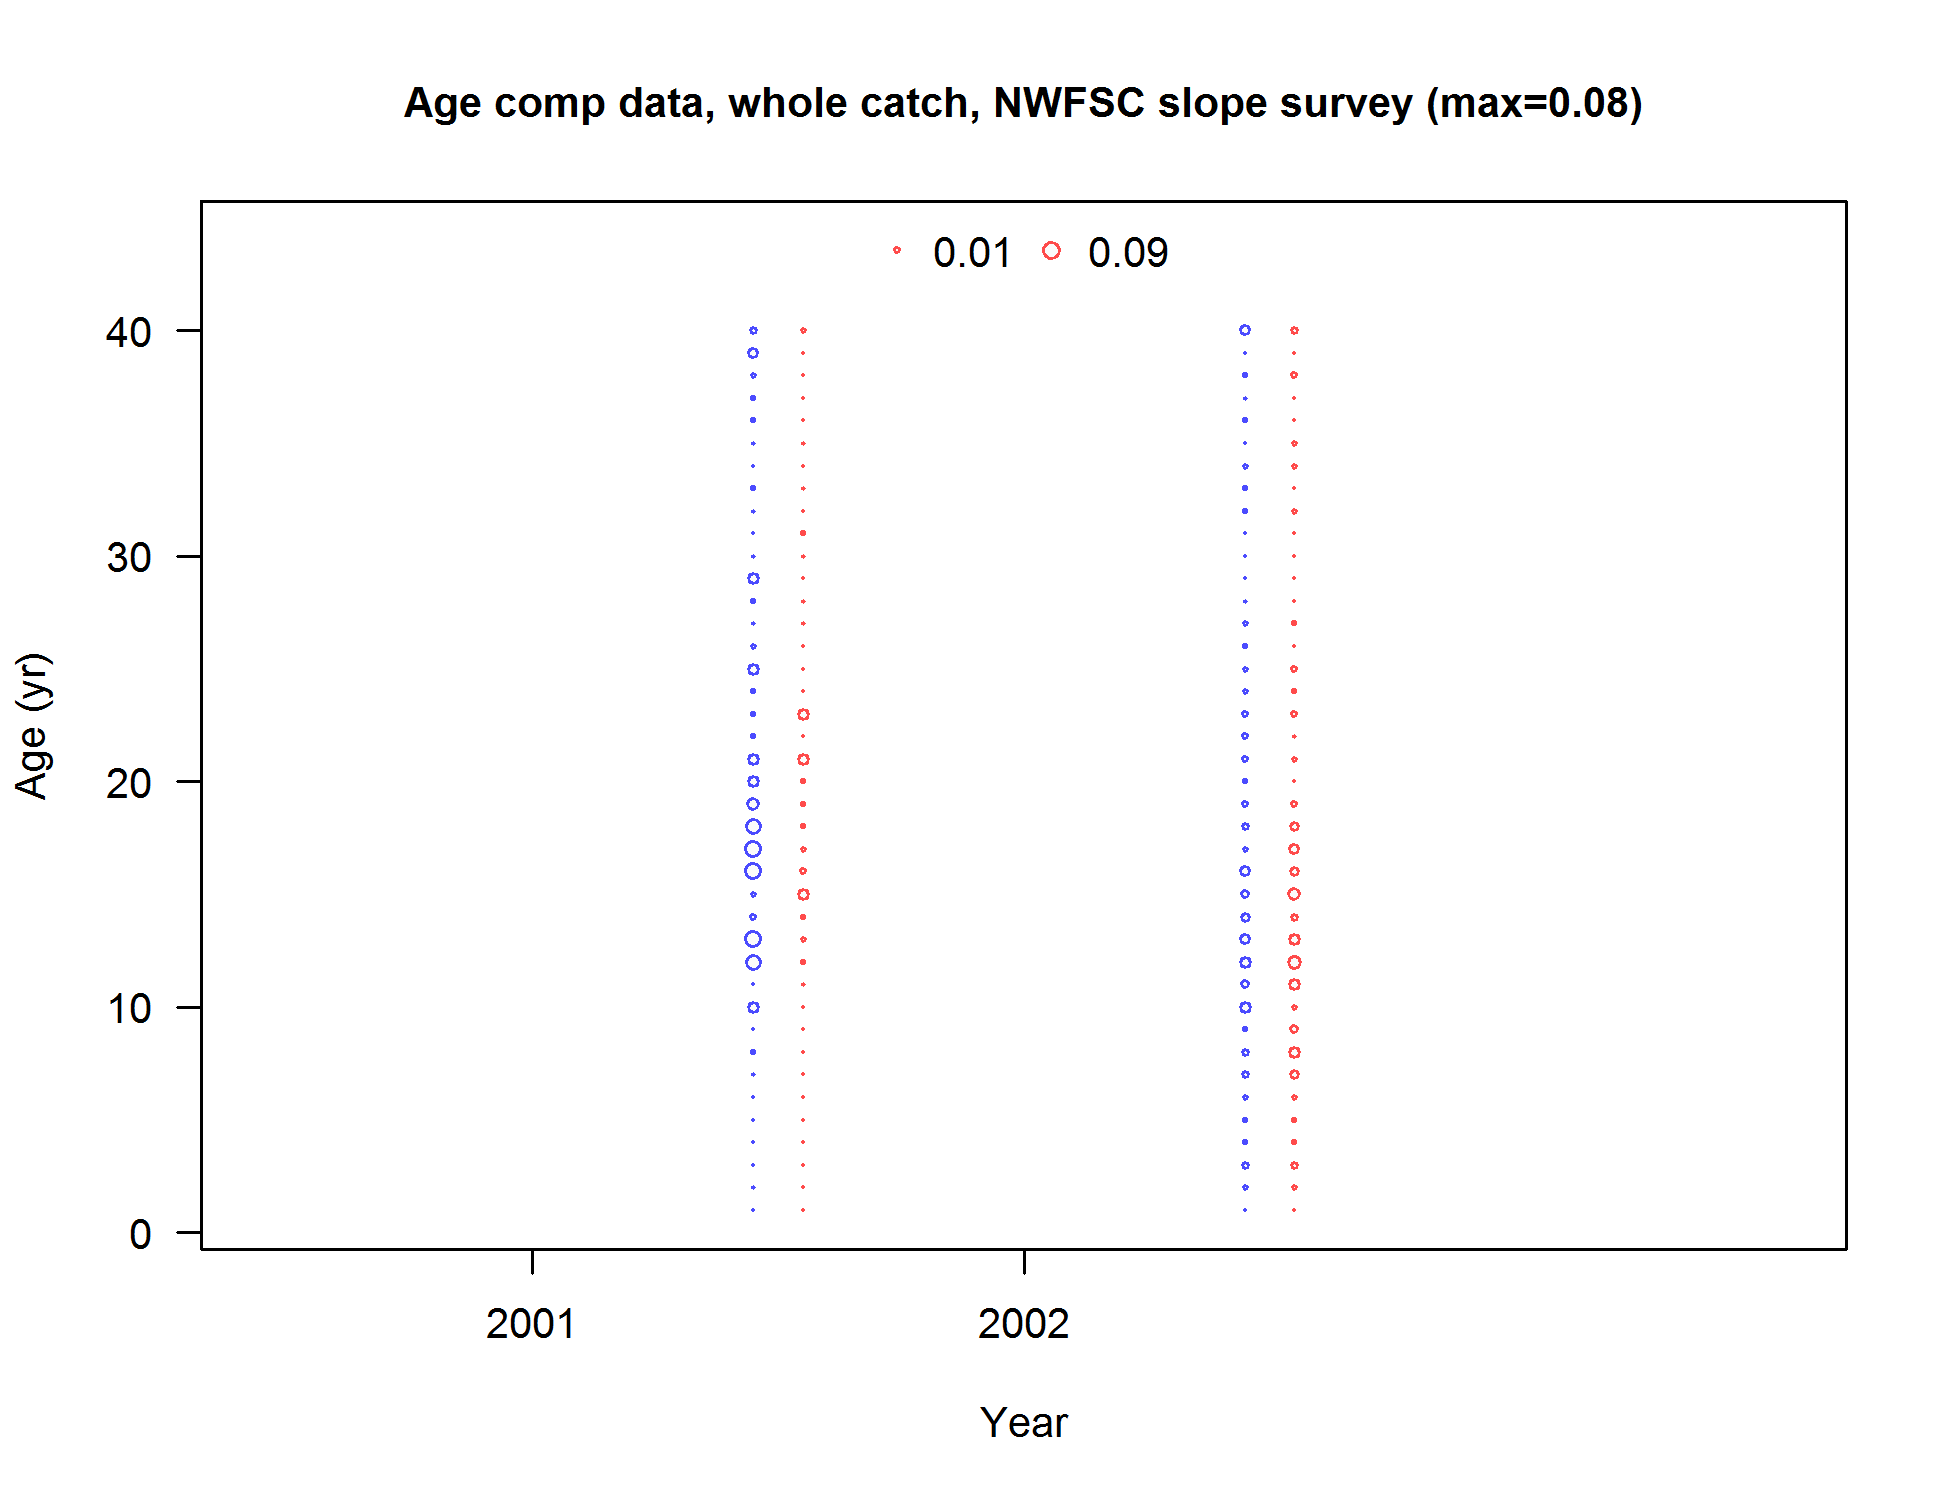
\includegraphics[scale = 0.50]{r4ss/comp_agedat_bubflt7mkt0.png}
  \end{center}
\end{frame}

\begin{frame}{NWFSC shelf-slope conditional age-at-length}
  \begin{center}
    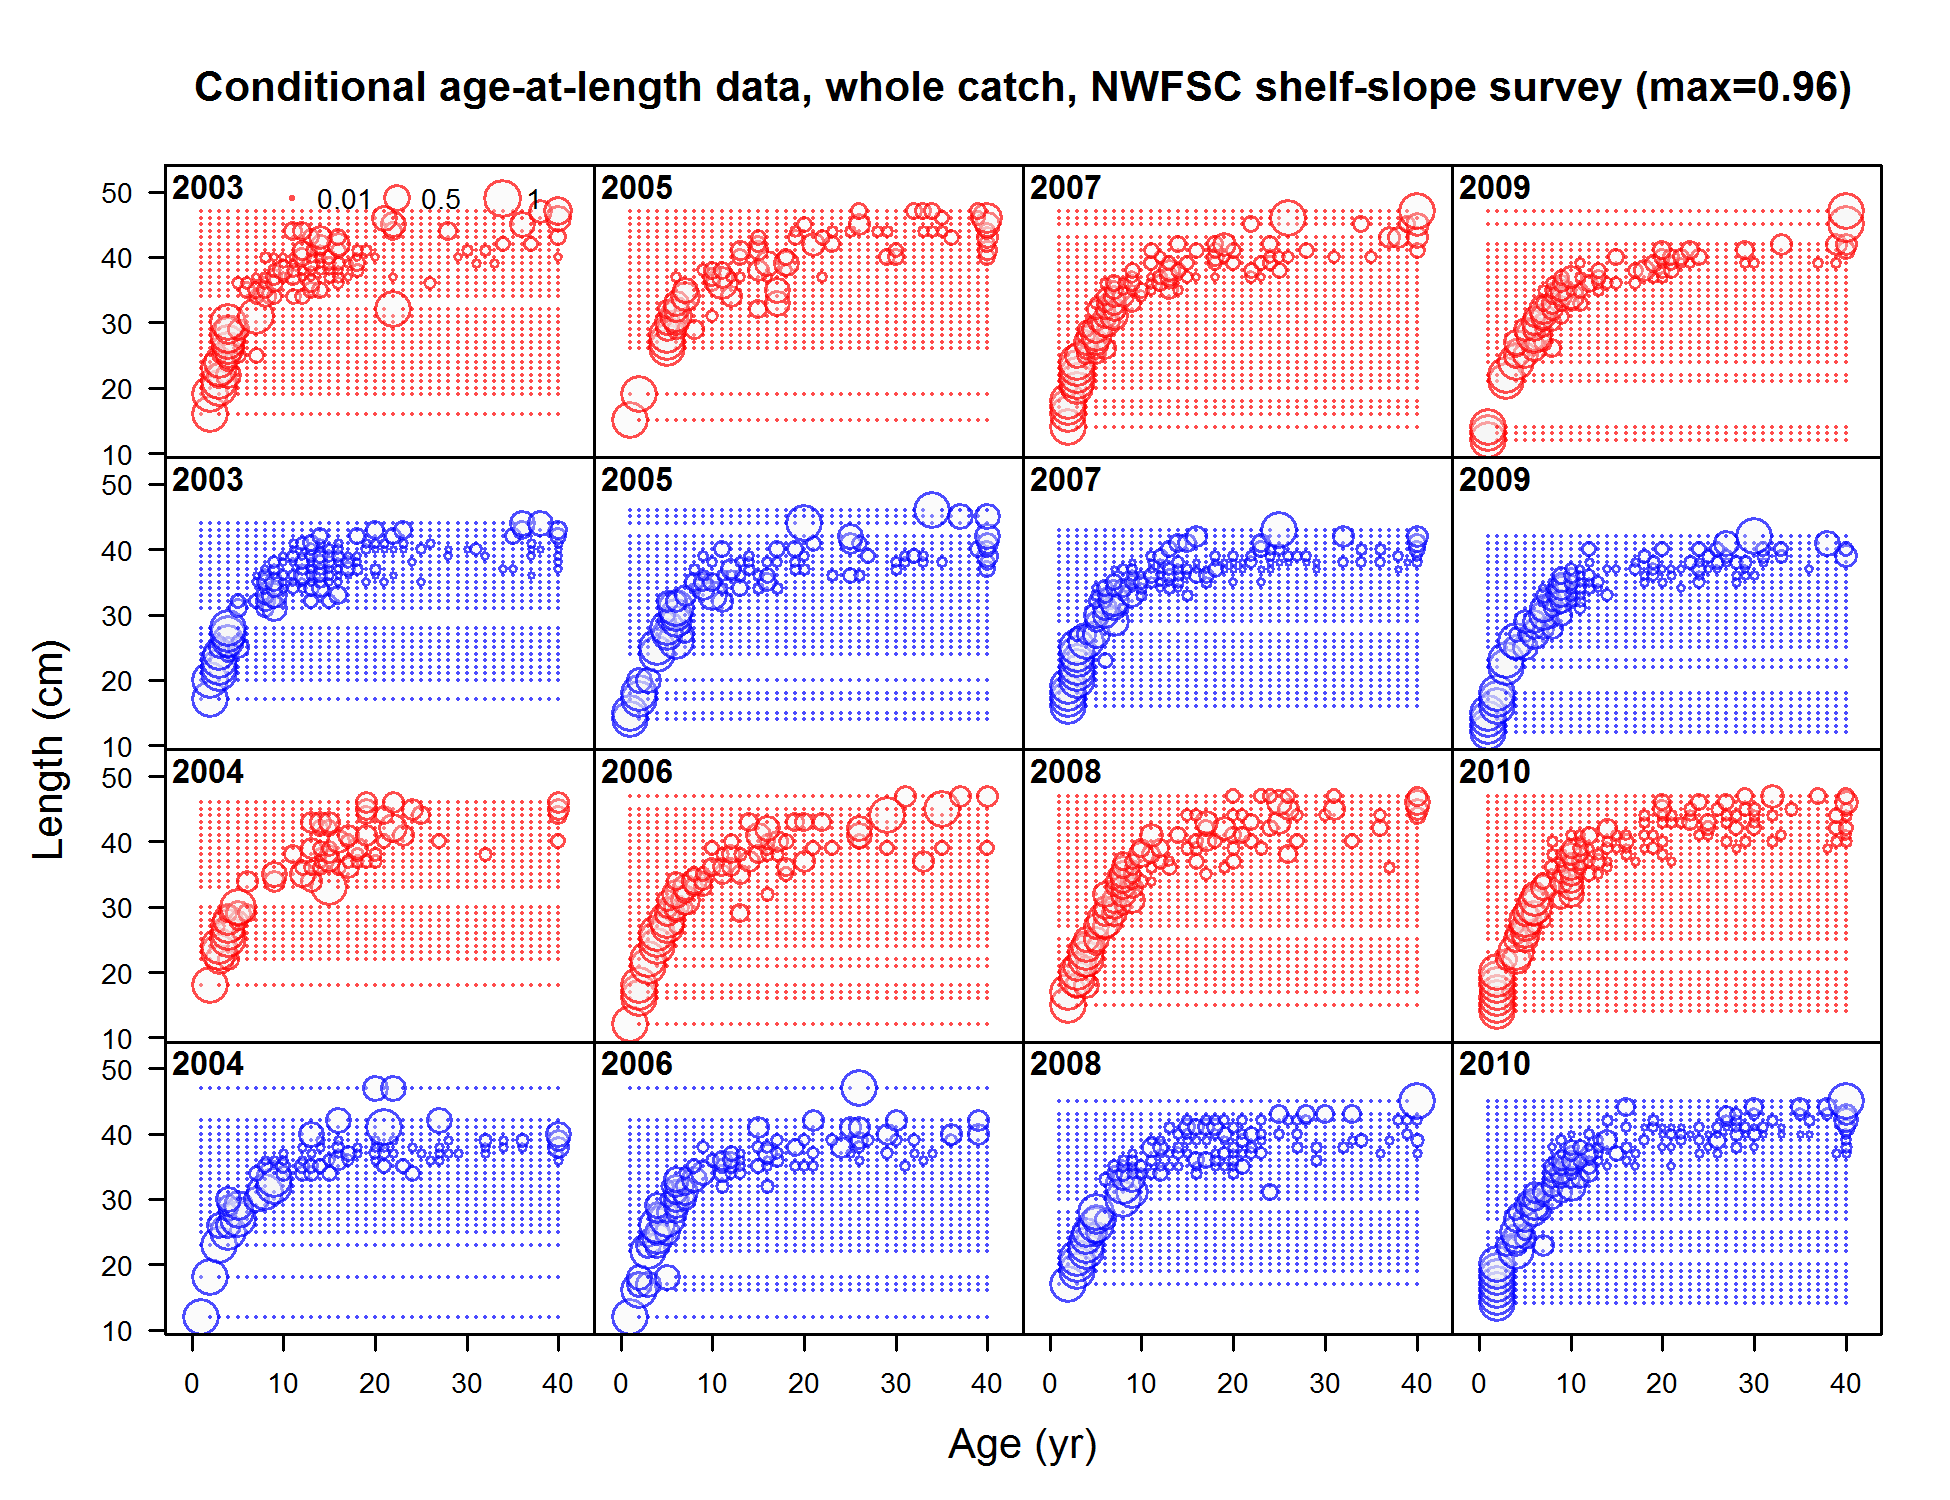
\includegraphics[scale = 0.50]{r4ss/comp_condAALdat_bubflt8mkt0_page1.png}
  \end{center}
\end{frame}

\begin{frame}{NWFSC shelf-slope conditional age-at-length}
  \begin{center}
    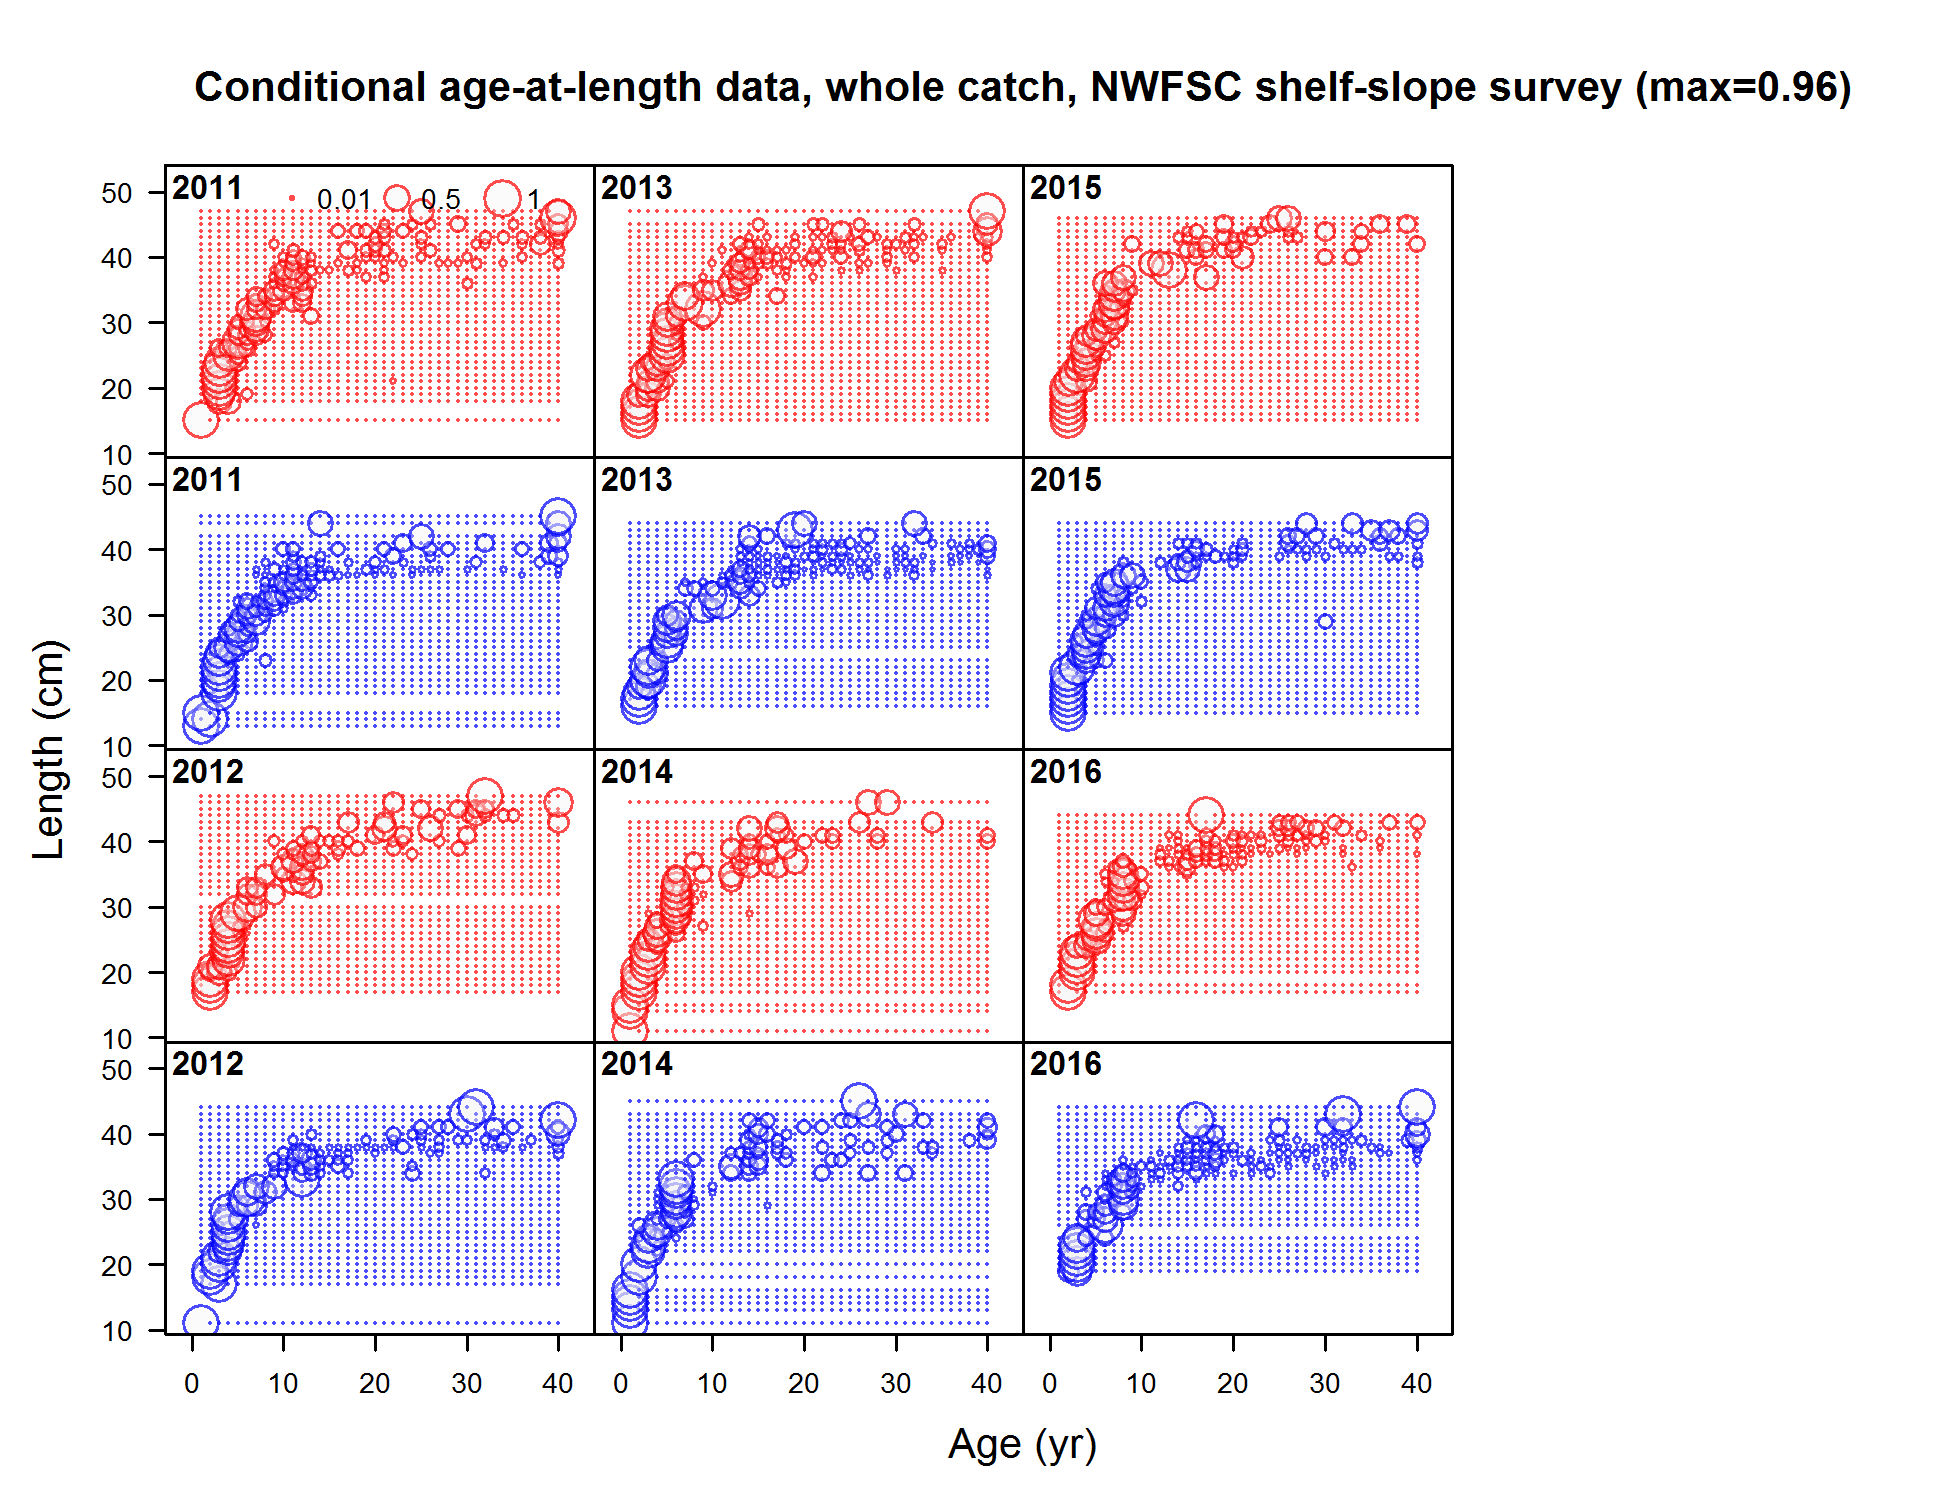
\includegraphics[scale = 0.50]{r4ss/comp_condAALdat_bubflt8mkt0_page2.png}
  \end{center}
\end{frame}

\begin{frame}{NWFSC shelf-slope ages - marginal view}
  \begin{center}
    \includegraphics[scale = 0.50]{r4ss/comp_gstagedat_bubflt8mkt0.png}
  \end{center}
\end{frame}


\subsection{Ageing Error}
\begin{frame}{Estimated Ageing Error: Curvilinear without bias}
  \begin{center}
    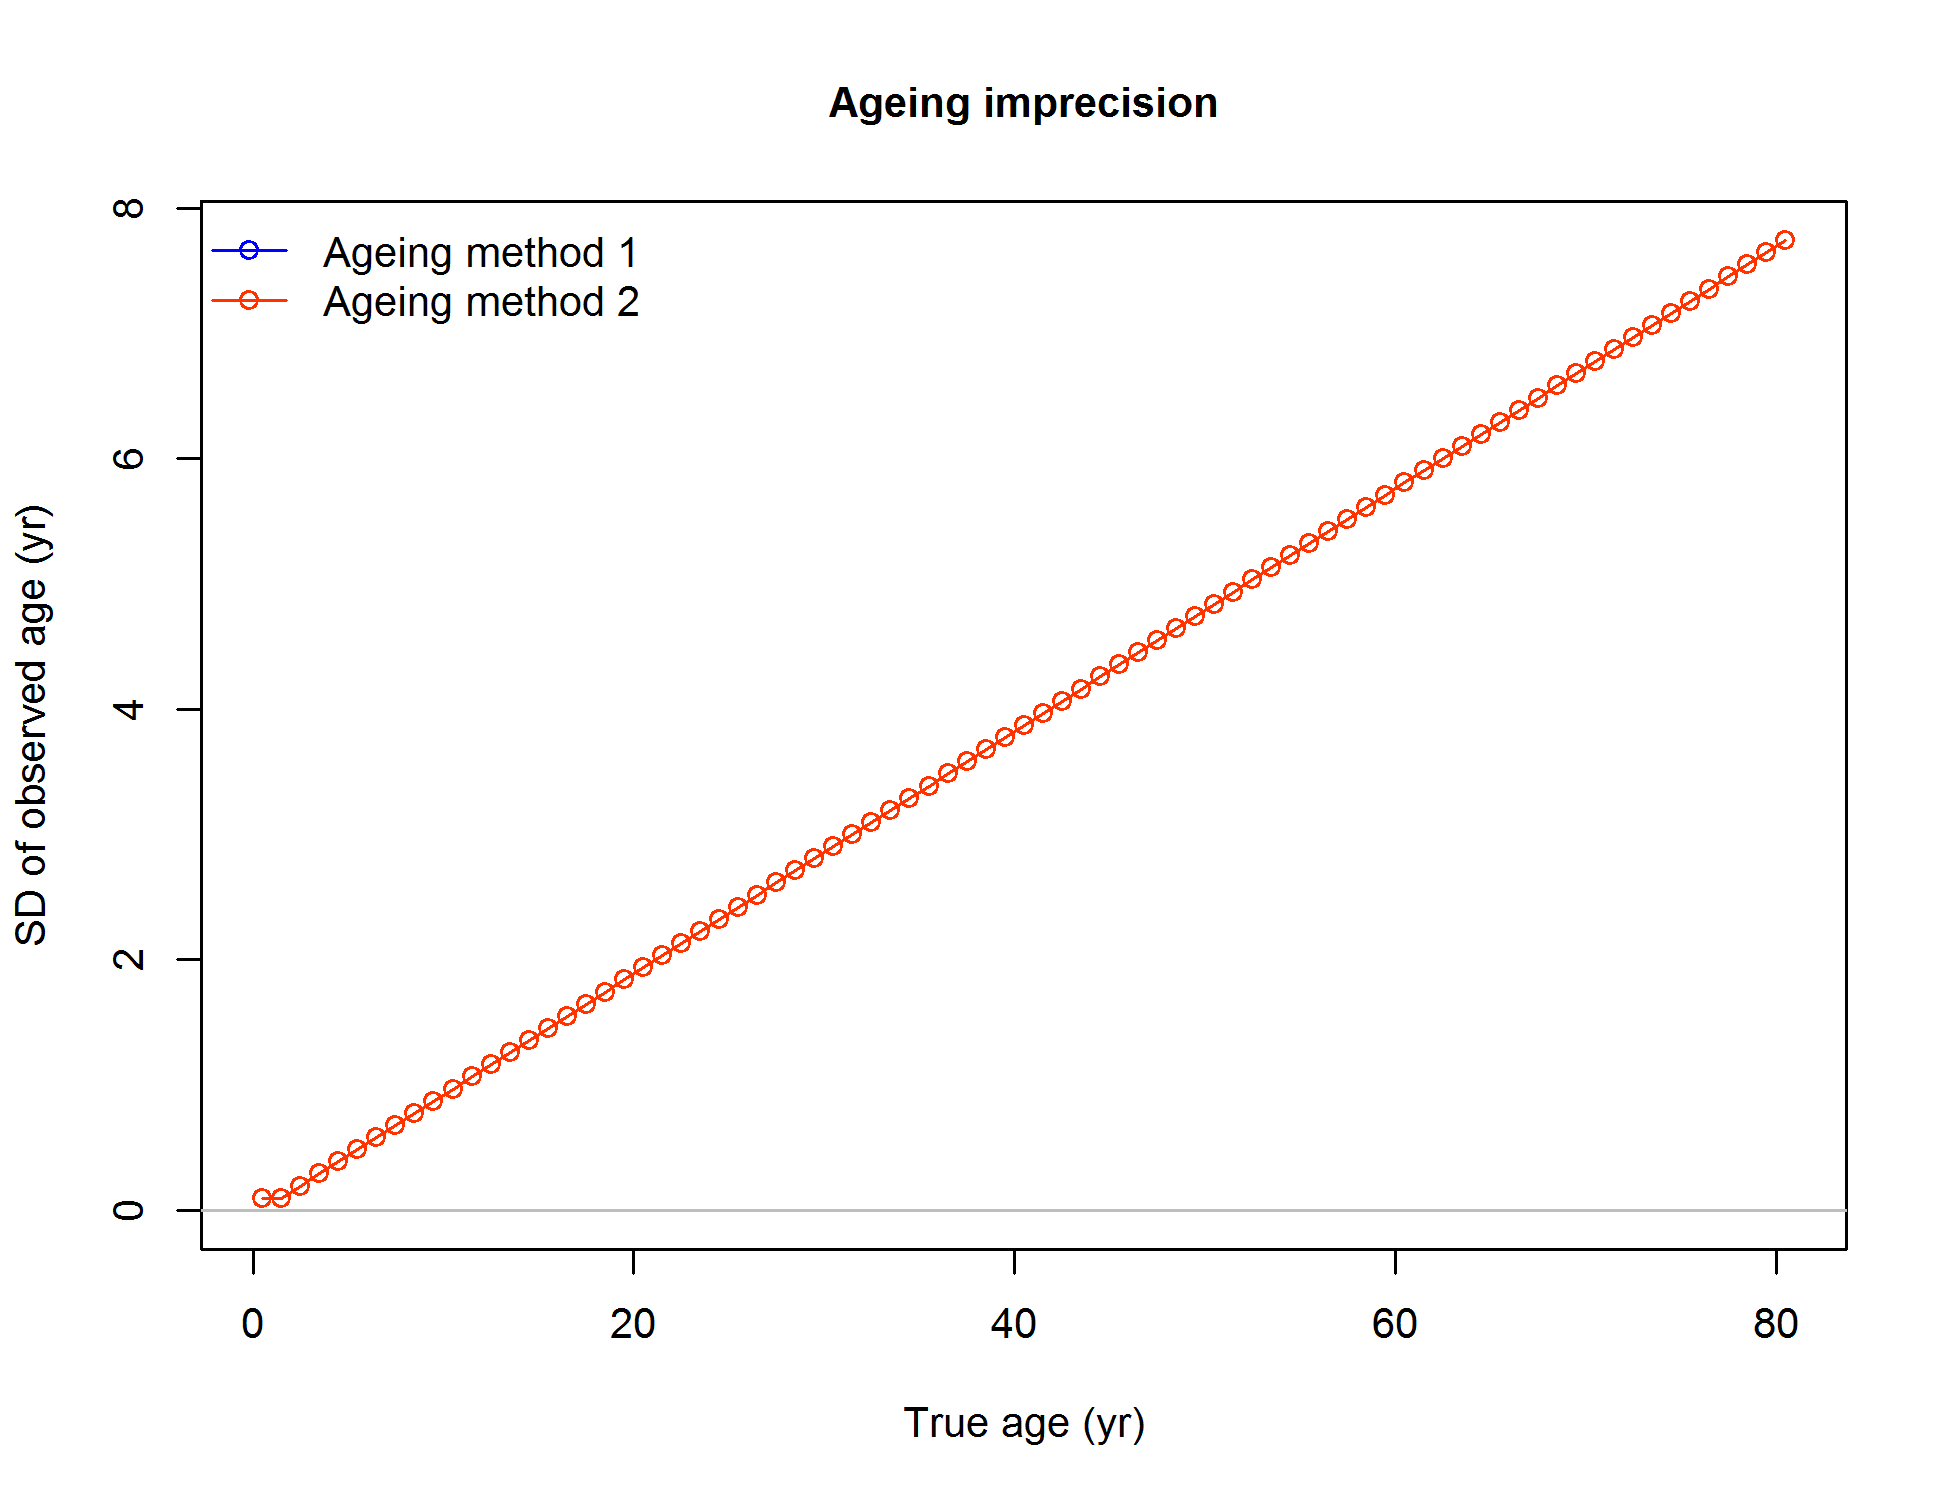
\includegraphics[scale = 0.50]{r4ss/numbers5_ageerrorSD.png}
  \end{center}

\end{frame}

\end{document}
